%&preformat-disser
\RequirePackage[l2tabu,orthodox]{nag} % Раскомментировав, можно в логе получать рекомендации относительно правильного использования пакетов и предупреждения об устаревших и нерекомендуемых пакетах
% Формат А4, 14pt (ГОСТ Р 7.0.11-2011, 5.3.6)
\documentclass[a4paper,14pt,oneside,openany]{memoir}

\input{common/setup}            % общие настройки шаблона
%%% Проверка используемого TeX-движка %%%
\newif\ifxetexorluatex   % определяем новый условный оператор (http://tex.stackexchange.com/a/47579)
\ifxetex
    \xetexorluatextrue
\else
    \ifluatex
        \xetexorluatextrue
    \else
        \xetexorluatexfalse
    \fi
\fi

\newif\ifsynopsis           % Условие, проверяющее, что документ --- автореферат

\usepackage{etoolbox}[2015/08/02]   % Для продвинутой проверки разных условий
\providebool{presentation}

\usepackage{comment}    % Позволяет убирать блоки текста (добавляет
                        % окружение comment и команду \excludecomment)

%%% Поля и разметка страницы %%%
\usepackage{pdflscape}  % Для включения альбомных страниц
\usepackage{geometry}   % Для последующего задания полей

%%% Математические пакеты %%%
\usepackage{amsthm,amsmath,amscd}   % Математические дополнения от AMS
\usepackage{amsfonts,amssymb}       % Математические дополнения от AMS
\usepackage{mathtools}              % Добавляет окружение multlined
\usepackage{gensymb}
\usepackage{textcomp}
\usepackage{rotating}
\usepackage{xfrac}                  % Красивые дроби
\usepackage[
    locale = DE,
    list-separator       = {;\,},
    list-final-separator = {;\,},
    list-pair-separator  = {;\,},
    list-units           = single,
    range-units          = single,
    range-phrase={\text{\ensuremath{-}}},
    % quotient-mode        = fraction, % красивые дроби могут не соответствовать ГОСТ
    fraction-function    = \sfrac,
    separate-uncertainty,
    ]{siunitx}[=v2]                 % Размерности SI
\sisetup{inter-unit-product = \ensuremath{{}\cdot{}}}

% Кириллица в нумерации subequations
% Для правильной работы требуется выполнение сразу после загрузки пакетов
\patchcmd{\subequations}{\def\theequation{\theparentequation\alph{equation}}}
{\def\theequation{\theparentequation\asbuk{equation}}}
{\typeout{subequations patched}}{\typeout{subequations not patched}}

%%%% Установки для размера шрифта 14 pt %%%%
%% Формирование переменных и констант для сравнения (один раз для всех подключаемых файлов)%%
%% должно располагаться до вызова пакета fontspec или polyglossia, потому что они сбивают его работу
\newlength{\curtextsize}
\newlength{\bigtextsize}
\setlength{\bigtextsize}{13.9pt}

\makeatletter
%\show\f@size    % неплохо для отслеживания, но вызывает стопорение процесса,
                 % если документ компилируется без команды  -interaction=nonstopmode
\setlength{\curtextsize}{\f@size pt}
\makeatother

%%% Кодировки и шрифты %%%
\ifxetexorluatex
    \ifpresentation
        \providecommand*\autodot{} % quick fix for polyglossia 1.50
    \fi
    \PassOptionsToPackage{no-math}{fontspec}    % https://tex.stackexchange.com/a/26295/104425
    \usepackage{polyglossia}[2014/05/21]        % Поддержка многоязычности
                                        % (fontspec подгружается автоматически)
\else
   %%% Решение проблемы копирования текста в буфер кракозябрами
    \ifnumequal{\value{usealtfont}}{0}{}{
        \input glyphtounicode.tex
        \input glyphtounicode-cmr.tex %from pdfx package
        \pdfgentounicode=1
    }
    \usepackage{cmap}   % Улучшенный поиск русских слов в полученном pdf-файле
    \ifnumequal{\value{usealtfont}}{2}{}{
        \defaulthyphenchar=127  % Если стоит до fontenc, то переносы
                                % не впишутся в выделяемый текст при
                                % копировании его в буфер обмена
    }
    \usepackage{textcomp}
    \usepackage[T1,T2A]{fontenc}                    % Поддержка русских букв
    \ifnumequal{\value{usealtfont}}{1}{% Используется pscyr, при наличии
        \IfFileExists{pscyr.sty}{\usepackage{pscyr}}{}  % Подключение pscyr
    }{}
    \usepackage[utf8]{inputenc}[2014/04/30]         % Кодировка utf8
    \usepackage[english, russian]{babel}[2014/03/24]% Языки: русский, английский
    \makeatletter\AtBeginDocument{\let\@elt\relax}\makeatother % babel 3.40 fix
    \ifnumequal{\value{usealtfont}}{2}{
        % http://dxdy.ru/post1238763.html#p1238763
        \usepackage[scaled=0.914]{XCharter}[2017/12/19] % Подключение русифицированных шрифтов XCharter
        \usepackage[charter, vvarbb, scaled=1.048]{newtxmath}[2017/12/14]
        \ifpresentation
        \else
            \setDisplayskipStretch{-0.078}
        \fi
    }{}
\fi

%%% Оформление абзацев %%%
\ifpresentation
\else
    \indentafterchapter     % Красная строка после заголовков типа chapter
    \usepackage{indentfirst}
\fi

%%% Цвета %%%
\ifpresentation
\else
    \usepackage[dvipsnames, table, hyperref]{xcolor} % Совместимо с tikz
\fi

%%% Таблицы %%%
\usepackage{longtable,ltcaption} % Длинные таблицы
\usepackage{multirow,makecell}   % Улучшенное форматирование таблиц
\usepackage{tabu, tabulary}      % таблицы с автоматически подбирающейся
                                 % шириной столбцов (tabu обязательно
                                 % до hyperref вызывать)
\makeatletter
%https://github.com/tabu-issues-for-future-maintainer/tabu/issues/26
\@ifpackagelater{longtable}{2020/02/07}{
\def\tabuendlongtrial{%
    \LT@echunk  \global\setbox\LT@gbox \hbox{\unhbox\LT@gbox}\kern\wd\LT@gbox
                \LT@get@widths
}%
}{}
\makeatother

\usepackage{threeparttable}      % автоматический подгон ширины подписи таблицы

%%% Общее форматирование
\usepackage{soulutf8}% Поддержка переносоустойчивых подчёркиваний и зачёркиваний
\usepackage{icomma}  % Запятая в десятичных дробях

%%% Оптимизация расстановки переносов и длины последней строки абзаца
\IfFileExists{impnattypo.sty}{% проверка установленности пакета impnattypo
    \ifluatex
        \ifnumequal{\value{draft}}{1}{% Черновик
            \usepackage[hyphenation, lastparline, nosingleletter, homeoarchy,
            rivers, draft]{impnattypo}
        }{% Чистовик
            \usepackage[hyphenation, lastparline, nosingleletter]{impnattypo}
        }
    \else
        \usepackage[hyphenation, lastparline]{impnattypo}
    \fi
}{}

%% Векторная графика

\usepackage{tikz}                   % Продвинутый пакет векторной графики
\usetikzlibrary{chains}             % Для примера tikz рисунка
\usetikzlibrary{shapes.geometric}   % Для примера tikz рисунка
\usetikzlibrary{shapes.symbols}     % Для примера tikz рисунка
\usetikzlibrary{arrows}             % Для примера tikz рисунка

%%% Гиперссылки %%%
\ifxetexorluatex
    \let\CYRDZE\relax
\fi
\usepackage{hyperref}[2012/11/06]

%%% Изображения %%%
\usepackage{graphicx}[2014/04/25]   % Подключаем пакет работы с графикой
\usepackage{caption}                % Подписи рисунков и таблиц
\usepackage{subcaption}             % Подписи подрисунков и подтаблиц
\usepackage{pdfpages}               % Добавление внешних pdf файлов

%%% Счётчики %%%
\usepackage{aliascnt}
\usepackage[figure,table]{totalcount}   % Счётчик рисунков и таблиц
\usepackage{totcount}   % Пакет создания счётчиков на основе последнего номера
                        % подсчитываемого элемента (может требовать дважды
                        % компилировать документ)
\usepackage{totpages}   % Счётчик страниц, совместимый с hyperref (ссылается
                        % на номер последней страницы). Желательно ставить
                        % последним пакетом в преамбуле

%%% Продвинутое управление групповыми ссылками (пока только формулами) %%%
\ifpresentation
\else
    \usepackage[russian]{cleveref} % cleveref имеет сложности со считыванием
    % языка из babel. Такое решение русификации вывода выбрано вместо
    % определения в documentclass из опасности что-то лишнее передать во все
    % остальные пакеты, включая библиографию.

    % Добавление возможности использования пробелов в \labelcref
    % https://tex.stackexchange.com/a/340502/104425
    \usepackage{kvsetkeys}
    \makeatletter
    \let\org@@cref\@cref
    \renewcommand*{\@cref}[2]{%
        \edef\process@me{%
            \noexpand\org@@cref{#1}{\zap@space#2 \@empty}%
        }\process@me
    }
    \makeatother
\fi

\usepackage{placeins} % для \FloatBarrier

\ifnumequal{\value{draft}}{1}{% Черновик
    \usepackage[firstpage]{draftwatermark}
    \SetWatermarkText{DRAFT}
    \SetWatermarkFontSize{14pt}
    \SetWatermarkScale{15}
    \SetWatermarkAngle{45}
}{}

%%% Цитата, не приводимая в автореферате:
% возможно, актуальна только для biblatex
%\newcommand{\citeinsynopsis}[1]{\ifsynopsis\else ~\cite{#1} \fi}

% если текущий процесс запущен библиотекой tikz-external, то прекомпиляция должна быть включена
\ifdefined\tikzexternalrealjob
    \setcounter{imgprecompile}{1}
\fi

\ifnumequal{\value{imgprecompile}}{1}{% Только если у нас включена предкомпиляция
    \usetikzlibrary{external}   % подключение возможности предкомпиляции
    \tikzexternalize[prefix=images/cache/,optimize command away=\includepdf] % activate! % здесь можно указать отдельную папку для скомпилированных файлов
    \ifxetex
        \tikzset{external/up to date check={diff}}
    \fi
}{}
         % Пакеты общие для диссертации и автореферата
\synopsisfalse                      % Этот документ --- не автореферат
\input{Dissertation/dispackages}    % Пакеты для диссертации
\input{Dissertation/userpackages}   % Пакеты для специфических пользовательских задач

\input{Dissertation/setup}      % Упрощённые настройки шаблона

% Новые переменные, которые могут использоваться во всём проекте
% ГОСТ 7.0.11-2011
% 9.2 Оформление текста автореферата диссертации
% 9.2.1 Общая характеристика работы включает в себя следующие основные структурные
% элементы:
% актуальность темы исследования;
\newcommand{\actualityTXT}{Актуальность темы.}
% степень ее разработанности;
\newcommand{\progressTXT}{Степень разработанности темы.}
% цели и задачи;
\newcommand{\aimTXT}{Целью}
\newcommand{\tasksTXT}{задачи}
% научную новизну;
\newcommand{\noveltyTXT}{Научная новизна.}
% теоретическую и практическую значимость работы;
%\newcommand{\influenceTXT}{Теоретическая и практическая значимость}
% или чаще используют просто
% \newcommand{\influenceTXT}{Практическая значимость}
\newcommand{\influenceTXT}{Научная значимость.}
% методологию и методы исследования;
\newcommand{\methodsTXT}{Методология и методы исследования.}
% положения, выносимые на защиту;
\newcommand{\defpositionsTXT}{Основные положения, выносимые на~защиту:}
% степень достоверности и апробацию результатов.
\newcommand{\reliabilityTXT}{Достоверность полученных результатов.}
\newcommand{\probationTXT}{Апробация работы.}

\newcommand{\contributionTXT}{Личный вклад.}
\newcommand{\publicationsTXT}{Публикации и апробация результатов.}


%%% Заголовки библиографии:

% для автореферата:
\newcommand{\bibtitleauthor}{Публикации автора по теме диссертации}

% для стиля библиографии `\insertbiblioauthorgrouped`
\newcommand{\bibtitleauthorvak}{В изданиях из списка ВАК РФ}
\newcommand{\bibtitleauthorscopus}{В изданиях, входящих в международную базу цитирования Scopus}
\newcommand{\bibtitleauthorwos}{В изданиях, входящих в международную базу цитирования Web of Science}
\newcommand{\bibtitleauthorother}{В прочих изданиях}
\newcommand{\bibtitleauthorconf}{В сборниках трудов конференций}
\newcommand{\bibtitleauthorpatent}{Зарегистрированные патенты}
\newcommand{\bibtitleauthorprogram}{Зарегистрированные программы для ЭВМ}

% для стиля библиографии `\insertbiblioauthorimportant`:
\newcommand{\bibtitleauthorimportant}{Наиболее значимые \protect\MakeLowercase\bibtitleauthor}

% для списка литературы в диссертации и списка чужих работ в автореферате:
\newcommand{\bibtitlefull}{Список литературы} % (ГОСТ Р 7.0.11-2011, 4)

\newcommand{\figRef}[1]{рис.~\ref{#1}}
\newcommand{\FigRef}[1]{Рис.~\ref{#1}}

\newcommand{\kelec}{\frac{1}{4\pi\varepsilon_0}}
\newcommand{\highlight}[1]{\textit{\textbf{#1}}}         % Новые переменные, для всего проекта

%%% Основные сведения %%%
\newcommand{\thesisAuthorLastName}{Булатов}
\newcommand{\thesisAuthorOtherNames}{Алексей Андреевич}
\newcommand{\thesisAuthorInitials}{А.\,А.}
\newcommand{\thesisAuthor}             % Диссертация, ФИО автора
{%
    \texorpdfstring{% \texorpdfstring takes two arguments and uses the first for (La)TeX and the second for pdf
        \thesisAuthorLastName~\thesisAuthorOtherNames% так будет отображаться на титульном листе или в тексте, где будет использоваться переменная
    }{%
        \thesisAuthorLastName, \thesisAuthorOtherNames% эта запись для свойств pdf-файла. В таком виде, если pdf будет обработан программами для сбора библиографических сведений, будет правильно представлена фамилия.
    }
}
\newcommand{\thesisAuthorShort}        % Диссертация, ФИО автора инициалами
{\thesisAuthorInitials~\thesisAuthorLastName}
%\newcommand{\thesisUdk}                % Диссертация, УДК
%{\fixme{xxx.xxx}}
\newcommand{\thesisTitle}              % Диссертация, название
{\fixme{Развитие радиофизических методов исследования динамики грозовых разрядов}}
\newcommand{\thesisSpecialtyNumber}    % Диссертация, специальность, номер
{01.04.03}
\newcommand{\thesisSpecialtyTitle}     % Диссертация, специальность, название (название взято с сайта ВАК для примера)
{Радиофизика}
%% \newcommand{\thesisSpecialtyTwoNumber} % Диссертация, вторая специальность, номер
%% {\fixme{XX.XX.XX}}
%% \newcommand{\thesisSpecialtyTwoTitle}  % Диссертация, вторая специальность, название
%% {\fixme{Теория и~методика физического воспитания, спортивной тренировки,
%% оздоровительной и~адаптивной физической культуры}}
\newcommand{\thesisDegree}             % Диссертация, ученая степень
{кандидата физико-математических наук}
\newcommand{\thesisDegreeShort}        % Диссертация, ученая степень, краткая запись
{канд. физ.-мат. наук}
\newcommand{\thesisCity}               % Диссертация, город написания диссертации
{Н.\,Новгород}
\newcommand{\thesisYear}               % Диссертация, год написания диссертации
{\the\year}
\newcommand{\thesisOrganization}       % Диссертация, организация
{Федеральное государственное бюджетное научное учреждение <<Федеральный исследовательский центр Институт прикладной физики Российской академии наук <<ИПФ РАН>>}
\newcommand{\thesisOrganizationShort}  % Диссертация, краткое название организации для доклада
{\fixme{НазУчДисРаб}}

\newcommand{\thesisInOrganization}     % Диссертация, организация в предложном падеже: Работа выполнена в ...
{\fixme{учреждении с~длинным длинным длинным длинным названием, в~котором
выполнялась данная диссертационная работа}}

%% \newcommand{\supervisorDead}{}           % Рисовать рамку вокруг фамилии
\newcommand{\supervisorFio}              % Научный руководитель, ФИО
{\fixme{Фамилия Имя Отчество}}
\newcommand{\supervisorRegalia}          % Научный руководитель, регалии
{\fixme{уч. степень, уч. звание}}
\newcommand{\supervisorFioShort}         % Научный руководитель, ФИО
{\fixme{И.\,О.~Фамилия}}
\newcommand{\supervisorRegaliaShort}     % Научный руководитель, регалии
{\fixme{к.~ф.-м.~н.,~уч.~зв.}}

%% \newcommand{\supervisorTwoDead}{}        % Рисовать рамку вокруг фамилии
%% \newcommand{\supervisorTwoFio}           % Второй научный руководитель, ФИО
%% {\fixme{Фамилия Имя Отчество}}
%% \newcommand{\supervisorTwoRegalia}       % Второй научный руководитель, регалии
%% {\fixme{уч. степень, уч. звание}}
%% \newcommand{\supervisorTwoFioShort}      % Второй научный руководитель, ФИО
%% {\fixme{И.\,О.~Фамилия}}
%% \newcommand{\supervisorTwoRegaliaShort}  % Второй научный руководитель, регалии
%% {\fixme{уч.~ст.,~уч.~зв.}}

\newcommand{\opponentOneFio}           % Оппонент 1, ФИО
{\fixme{Фамилия Имя Отчество}}
\newcommand{\opponentOneRegalia}       % Оппонент 1, регалии
{\fixme{доктор физико-математических наук, профессор}}
\newcommand{\opponentOneJobPlace}      % Оппонент 1, место работы
{\fixme{Не очень длинное название для места работы}}
\newcommand{\opponentOneJobPost}       % Оппонент 1, должность
{\fixme{старший научный сотрудник}}

\newcommand{\opponentTwoFio}           % Оппонент 2, ФИО
{\fixme{Фамилия Имя Отчество}}
\newcommand{\opponentTwoRegalia}       % Оппонент 2, регалии
{\fixme{кандидат физико-математических наук}}
\newcommand{\opponentTwoJobPlace}      % Оппонент 2, место работы
{\fixme{Основное место работы c длинным длинным длинным длинным названием}}
\newcommand{\opponentTwoJobPost}       % Оппонент 2, должность
{\fixme{старший научный сотрудник}}

%% \newcommand{\opponentThreeFio}         % Оппонент 3, ФИО
%% {\fixme{Фамилия Имя Отчество}}
%% \newcommand{\opponentThreeRegalia}     % Оппонент 3, регалии
%% {\fixme{кандидат физико-математических наук}}
%% \newcommand{\opponentThreeJobPlace}    % Оппонент 3, место работы
%% {\fixme{Основное место работы c длинным длинным длинным длинным названием}}
%% \newcommand{\opponentThreeJobPost}     % Оппонент 3, должность
%% {\fixme{старший научный сотрудник}}

\newcommand{\leadingOrganizationTitle} % Ведущая организация, дополнительные строки. Удалить, чтобы не отображать в автореферате
{\fixme{Федеральное государственное бюджетное образовательное учреждение высшего
профессионального образования с~длинным длинным длинным длинным названием}}

\newcommand{\defenseDate}              % Защита, дата
{\fixme{DD mmmmmmmm YYYY~г.~в~XX часов}}
\newcommand{\defenseCouncilNumber}     % Защита, номер диссертационного совета
{\fixme{Д\,123.456.78}}
\newcommand{\defenseCouncilTitle}      % Защита, учреждение диссертационного совета
{\fixme{Название учреждения}}
\newcommand{\defenseCouncilAddress}    % Защита, адрес учреждение диссертационного совета
{\fixme{Адрес}}
\newcommand{\defenseCouncilPhone}      % Телефон для справок
{\fixme{+7~(0000)~00-00-00}}

\newcommand{\defenseSecretaryFio}      % Секретарь диссертационного совета, ФИО
{\fixme{Фамилия Имя Отчество}}
\newcommand{\defenseSecretaryRegalia}  % Секретарь диссертационного совета, регалии
{\fixme{д-р~физ.-мат. наук}}            % Для сокращений есть ГОСТы, например: ГОСТ Р 7.0.12-2011 + http://base.garant.ru/179724/#block_30000

\newcommand{\synopsisLibrary}          % Автореферат, название библиотеки
{\fixme{Название библиотеки}}
\newcommand{\synopsisDate}             % Автореферат, дата рассылки
{\fixme{DD mmmmmmmm}\the\year~года}

% To avoid conflict with beamer class use \providecommand
\providecommand{\keywords}%            % Ключевые слова для метаданных PDF диссертации и автореферата
{}
             % Основные сведения
\input{common/fonts}            % Определение шрифтов (частичное)
\input{common/styles}           % Стили общие для диссертации и автореферата
\input{Dissertation/disstyles}  % Стили для диссертации
\input{Dissertation/userstyles} % Стили для специфических пользовательских задач

%%% Библиография. Выбор движка для реализации %%%
% Здесь только проверка установленного ключа. Сама настройка выбора движка
% размещена в common/setup.tex
\ifnumequal{\value{bibliosel}}{0}{%
    \input{biblio/predefined}   % Встроенная реализация с загрузкой файла через движок bibtex8
}{
    \input{biblio/biblatex}     % Реализация пакетом biblatex через движок biber
}

% Вывести информацию о выбранных опциях в лог сборки
\typeout{Selected options:}
\typeout{Draft mode: \arabic{draft}}
\typeout{Font: \arabic{fontfamily}}
\typeout{AltFont: \arabic{usealtfont}}
\typeout{Bibliography backend: \arabic{bibliosel}}
\typeout{Precompile images: \arabic{imgprecompile}}
% Вывести информацию о версиях используемых библиотек в лог сборки
\listfiles

%%% Управление компиляцией отдельных частей диссертации %%%
% Необходимо сначала иметь полностью скомпилированный документ, чтобы все
% промежуточные файлы были в наличии
% Затем, для вывода отдельных частей можно воспользоваться командой \includeonly
% Ниже примеры использования команды:
%
%\includeonly{Dissertation/part2}
%\includeonly{Dissertation/contents,Dissertation/appendix,Dissertation/conclusion}
%
% Если все команды закомментированы, то документ будет выведен в PDF файл полностью

\begin{document}
%%% Переопределение именований типовых разделов
% https://tex.stackexchange.com/a/156050
\gappto\captionsrussian{\input{common/renames}\unskip} % for polyglossia and babel
\input{common/renames}

%%% Структура диссертации (ГОСТ Р 7.0.11-2011, 4)
\include{Dissertation/title}           % Титульный лист
\include{Dissertation/contents}        % Оглавление
\ifnumequal{\value{contnumfig}}{1}{}{\counterwithout{figure}{chapter}}
\ifnumequal{\value{contnumtab}}{1}{}{\counterwithout{table}{chapter}}
\include{Dissertation/introduction}    % Введение
\ifnumequal{\value{contnumfig}}{1}{\counterwithout{figure}{chapter}
}{\counterwithin{figure}{chapter}}
\ifnumequal{\value{contnumtab}}{1}{\counterwithout{table}{chapter}
}{\counterwithin{table}{chapter}}

\chapter{Региональная широкополосная грозопеленгационная система}
\label{sec:lds-intro}
Информация, собираемая грозопеленгационными системами, важна для решения задач оперативного мониторинга молниевой активности, краткосрочного прогноза быстроразвивающихся конвективных явлений, изучения климатологии молний и других прикладных и фундаментальных задач. Безопасность движения воздушных судов напрямую зависит от оперативной информации о молниевой активности, поскольку грозовые фронты являются помехами воздушному движению. Надежная молниезащита наземных объектов требует знания удельной поражаемости определенных территорий молниями, величин средних и максимальных токов разрядов, и других параметров. Зачастую грозы являются предвестниками развития опасных событий, таких, как шквал и катастрофические ливневые осадки, смерчи, град \cite{Matveev1984}. Например, быстрое увеличение числа внутриоблачных разрядов в единицу времени до 60~р/мин является признаком возникновения шквала или торнадо в течение 10-15 мин. Изменение преобладающей полярности молний с отрицательной на положительную является признаком начала формирования градовых частиц в облаке, а обратный процесс "--- об окончании градоопасной стадии \cite{Matveev1984}. С другой стороны, оперативные данные местоположения молний позволяют верифицировать прогнозные алгоритмы и реализовывать системы корректировки (<<nudging>>) численных моделей в соответствии с наблюдаемыми явлениями \cite{Huang2009}. 

Грозопеленгационные сети, совместно аэроэлектрическими наблюдениями \cite{Anisimov2013}, являются основой для задачи усвоения геоэлектрических метеоданных, исследований глобальной электрической цепи и климатологии молнии \cite{Mareev2010,Williams2014}. Статистика параметров молниевых разрядов напрямую связана с особенностями процессов, возникающих при инициации и развитии молнии, что позволяет развивать физику молниевого разряда. Совместное применение ГПС и других методов наблюдения за грозами порождает дополнительные возможности исследования окружающей природы.

Одним из путей развития мировой грозопеленгации является развертывание и совершенствование глобальных сетей местоопределения молниевых вспышек, основанных на приеме сверхдлинноволнового (СДВ) электромагнитного излучения. Лидирующие позиции в данном сегменте занимают сети WWLLN \cite{wwllnSite} и GLD360 \cite{gld360Site}. Однако, СДВ-системы обладают серьёзными недостатками: они регистрируют не более 20-30\% от общего числа вспышек облако-земля, имеют трудности с определением полярности молнии и не предоставляют информацию о внутриоблачных разрядах, что значительно затрудняет использование данных для оперативного мониторинга. Тем не менее, глобальные сети оказываются полезны для исследования климатологии молний, валидации глобальных и мезомасштабных прогнозов.

В настоящее время во всем мире активно развиваются региональные системы, позволяющие с высокой точностью фиксировать как разряды типа облако-земля, так и внутриоблачные разряды, и определять большое количество параметров вспышек \cite{Pinto2003,nldnSiteArticle}.

В данной главе приведён обзор существующих грозопеленгационных систем, а также описана разработанная автором регональная грозопеленгационная система OpenLDS \cite{BulatovMiG}. Система введена в эксплуатацию в течение конвективного сезона 2014 г. и работает в непрерывном режиме. Нижегородская ГПС является многопунктовой. Приёмники системы  работают в СДВ и ДВ-диапазоне. К конвективному сезону 2017~г. ГПС расширена до 6 пунктов пеленгации и покрывает область размерами порядка 1500~км. Проведена оценка точности разработанной системы на основании сравнения с данными международной ГПС WWLLN и показаниями ДМРЛ, установленного в Нижнем Новгороде. На основе показаний ГПС исследовано распределение гроз в регионе. Исследованы статистические особенности мультипликативности обратного удара и максимальных токов повторных разрядов.

\section{Классификация грозопеленгационных систем}
Грозопеленгационная система (ГПС) представляет собой ап\-па\-рат\-но-про\-грамм\-ный комплекс, предназначенный для определения положения молниевых разрядов в пространстве, времени их возникновения, а также их характеристик. Грозопеленгационные системы можно классифицировать по следующим признакам:
\begin{itemize}
	\item \textbf{Распределённость.} Однопунктовые системы содержат только одно устройство регистрации электромагнитного излучения (грозопеленгатор), а многопунктовые включают в себя несколько грозопеленгаторов, распределенных на некоторой площади. При этом данные, получаемые с разных грозопеленгаторов, обрабатываются совместно. Многопунктовые грозопеленгационные системы также называют грозопеленгационными сетями. Такие системы обладают большей точностью и надёжностью, однако их разработка сложнее, а стоимость развёртывания "--- больше.
	\item \textbf{Частотный диапазон.} Определяется диапазоном при\-ем\-ни\-ков-гро\-зо\-пе\-лен\-га\-то\-ров, используемых в системе. Широкое распространение имеют ГПС, работающие в СДВ-диапазоне. Приемники таких систем способны регистрировать разряды со всего земного шара (при достаточной чувствительности). Также, распространены ГПС, работающие в ДВ, КВ и УКВ диапазонах. 
	\item \textbf{Метод пеленгации.} Для определения положения молнии многопунктовыми ГПС наиболее часто применяются метод пересечения пеленгов (direction finding), разностно-дальномерный метод (time-of-arrival), а также их комбинации и модификации. Однопунктовые ГПС определяют пеленг молнии по горизонтальным компонентам магнитного поля, а расстояние "--- по разности фаз между магнитным и электрическим полем, интенсивности и другим параметрам сигнала.
	\item \textbf{Доступность данных.} Результаты работы ГПС могут быть доступны или недоступны для внешних исследователей. Доступ может осуществляться на платной, либо бесплатной основе с теми или иными ограничениями. Системы, ориентированные на финдаментальные исследования, предоставляют доступ к архиву данных за продолжительный срок, в то время как системы, ориентированные на оперативный мониторинг предоставляют данные с наименьшей задердкой. Также, имеет значение доступность первичных данных грозопеленгации: записей электромагнитных полей и временных меток приёмников. 
	\item \textbf{Открытость алгоритмов работы.} Большинство систем грозопеленгации не раскрывают деталей алгоритмов позиционирования разрядов, что затрудняет анализ данных.
\end{itemize}

Применительно к задачам грозопеленгации, выделяют следующие характеристики молниевых разрядов:
\begin{itemize}
	\item Тип разряда "--- внутриоблачный, либо облако-земля
	\item Знак заряда, переносимого из облака на землю "--- положительный, либо отрицательный
	\item Максимальный и средний токи молнии
	\item Величина перенесенного заряда
	\item Количество повторных обратных ударов
\end{itemize}
и другие характеристики. Устройство, предназначенное для регистрации в той или иной форме электромагнитного излучения молний называют грозопеленгатором.

\section{Существующие системы грозопеленгации}
\label{sec:lds-review}
На данный момент в мире функционирует несколько глобальных грозопеленгационных систем, охватывающих весь земной шар, и значительное число региональных, области покрытия которых имеют характерный размер от сотен до десятков тысяч километров. На территории России также развернуто несколько ГПС, отличающихся параметрами и назначением.

\subsection{Зарубежные и международные ГПС}
Рассмотрим особенности и характеристики наиболее значимых грозопеленгационных систем, разрабатываемых и поддерживаемых зарубежными коллегами.
% Информация здесь: https://link.springer.com/article/10.1007/s10712-013-9251-1#Sec18

\subsubsection{World Wide Lightning Location Network}
Грозопеленгационная система World Wide Lightning Location Network\cite{wwllnSite} (WWLLN, принятое русское произношение <<Вулин>>) "--- глобальная ГПС, поддерживаемая Университетом Вашингтона, Сиэтл. Основное назначение системы "--- научные исследования. Доступны данные с 15~августа~2014~года.

Система WWLLN объединяет более 70~грозопелегаторов по всему миру и работает в СДВ-диапазоне, 3--30\,КГц. Поскольку пеленгаторы находятся на достаточно большом удалении друг от друга, WWLLN обнаруживает только наиболее интенсивные молнии. Согласно \cite{wwllnSite}, только 15--30\%~разрядов, зарегистрированных одним грозопеленгатором, регистрируются не менее чем 4~другими. Для вспышек с пиковым током более~30\,кА регистрируется около 30\%~событий.

Для определения положений молниевых разрядов системой WWLLN применяется метод time of group arrival (<<TOGA>>) "--- разновидность разностно-дальномерного метода с модификациями, являющимися коммерческой тайной WWLLN.

На основе сравнения показаний системы WWLLN и системы OpenLDS, созданной в рамках данной работы, на территории Нижегородской области погрешность позиционирования разрядов WWLLN составляет, приблизительно, 4\,км с систематическим смещением с систематическим смещением 2,2\,км на северо-запад\cite{BulatovMiG}.

Важной аппаратной особенностью WWLLN, существенно ограничивающей её возможности, является применение звуковых карт персональных компьютеров в качестве АЦП пунктов грозопеленгации.

\subsubsection{U.\,S. National Lightning Detection Network}
U.\,S. National Lightning Detection Network\cite{nldnSiteArticle} (NLDN) "--- грозопеленгационная система, разработанная компанией Vaisala по заказу правительства США.

Система NLDN обладает высокой точностью на территории США и состоит из более чем 100~пунктов пеленгации, расположенных сеткой с характерным шагом 300--350\,км. Диапазон работы приёмников составляет 400\,Гц--400\,кГц. Регистрируются как разряды облако-земля, так и внутриоблачные. Максимальные токи молний определяются при помощи эмпирической формулы, основанной на данных триггерных молний. Согласно исследованию \cite{Biagi2007}, на территории Южной Аризоны NLDN регистрирует 76\% молний, а в Оклахоме, штат Техас "--- 85\%. \cite{Rakov-emld}

Для определения положения молний применяется комбинация разностно-дальномерного метода и метода пересечения пеленгов \cite{Rakov-emld}. Алгоритмы обработки данных системой NLDN закрыты и являются коммерческой тайной. 

\subsubsection{Global Lightning Dataset }
Global Lightning Dataset (GLD360), также называемая Global Lightning Detection Network (GLDN) "--- глобальная система СДВ-диапазона разработки компании Vaisala. 

Согласно \cite{Demetriades2010}, эффективность детектирования молний системой GLD360 на территории США составляет 86–92\% при средней ошибке позиционирования 10,8\,км. Однако согласно \cite{Naccarato2010}, на территории Бразилии система регистрирует около 16\% вспышек с ошибкой 12,5\,км. Помимо координат, система определяет максимальные токи и полярность молний, основываясь на записях электромагнитного поля. Определение типа разряда происходит посредством сравнения с известными <<каноническими>> сигналами. \cite{Rakov-emld}

Позиционирование молний происходит с использованием комбинации разностно-дальномерного метода и метода пересечения пеленгов \cite{Rakov-emld}. Данные GLD360 доступны по платной подписке. Алгоритмы работы системы не раскрываются.

\subsubsection{Earth Networks Total Lightning Network}
Система Earth Networks Total Lightning Network (ENTLN) действует на территории США и ряда другиз стран \cite{Rakov-emld}. Система работает в широкой полосе частот от 1\,Гц до 12\,МГц. Применяется разностно-дальномерный метод пеленгации. Сигнал с электрической антенны используется как для определения положения молний, так и для разделения разрядов по типу: внутриоблачные или облако-земля. Разряды удаленные не более, чем на 10\,км и отстоящие по времени не более, чем 700\, считаются относящимися к одной молнии. \cite{Heckman2010}

По заявлениям разработчиков \cite{Heckman2010}, система регистрирует 40--50\% внутриоблачных разрядов на большей части территории США и до 95\% на среднем западе и востоке США. Высокая чувствительность к внутриоблачным разрядам является приоритетом ENTLN.

\subsection{Отечественные ГПС и исследования на их основе}
Обзор основных результатов российских исследователей в области грозопеленгации на 2015\,г. представлен в обзоре\cite{MareevWe2016}.

На территории нашей страны также развиваются системы многопунктовой грозопеленгации. Проводятся работы по исследованию и улучшению показателей точности существующих систем \cite{Kononov2014,Kononov2013}, разрабатываются новые системы и комплексы \cite{Adjiev2013,BulatovMiG}. Проводятся исследования, использующие данные грозопеленгации отдельно, а также совместно с другими источниками информации о молниевой активности \cite{Buharov2013}.

На территории Северного Кавказа впервые в России введен в эксплуатацию грозорегистратор LS 8000 фирмы «Vaisala». Он обеспечивает определение координат, полярности, типа (облако-облако или облако-земля), токов и других характеристик молниевых разрядов. Предполагается совместная кластерная обработка данных LS 8000 с картой радиоэха облаков и осадков, полученной региональной сетью МРЛ в реальном времени. За период эксплуатации грозорегистратора LS 8000 с 2008 г. проведены исследования параметров токов зарегистрированных разрядов облако-земля. \cite{Adjiev2013} 

В течение 2011 г. модифицирована грозопеленгационная система <<Алвес 9.07>>\cite{AlwesSite}, разработанная ООО <<Алвес>>, совместно с сотрудниками отдела Атмосферного электричества Главной геофизической обсерватории. Система <<Алвес>> основанная на разностно-дальномерном принципе и покрывает территорию Европейской части России и Урал. Разработано и внедрено новое поколение грозорегистраторов. По данным на август 2014 г. в состав системы входят 70 разнесенных пунктов регистрации гроз. В течение конвективных сезонов 2013-2014 гг. проведены оценки точностных характеристик сети с использованием данных локации грозовых очагов европейской разностно-дальномерной сети Blitzortung \cite{Snegurov2010, AlwesSite}. Также, исследованы источники ошибок, обусловленные погрешностями временной привязки к сигналам атмосфериков в разнесенных пунктах системы. Произведены модельные и экспериментальные оценки величин этих погрешностей \cite{Kononov2011, Kononov2014}. Проведены модельные оценки погрешностей алгоритмов однопунктового определения координат сильноточного молниевого разряда в рамках его модели в виде произвольно ориентированного электрического диполя, обусловленных влиянием внешних атмосферных и индустриальных помех \cite{Kononov2013}.

На востоке Сибири исследованы особенности пространственного распределения положительных грозовых разрядов за 2003-2007 гг., зафиксированных однопунктовым грозопеленгатором-дальномером с радиусом наблюдения около 1200 км. Зафиксировано, что распределения положительных разрядов в целом отражают общую картину грозовой активности. Выделены области очагов грозовой активности, в которых отношение потока положительных разрядов к потоку отрицательных может превышать 1, что обусловлено географическими условиями — высокогорной местностью и близостью Охотского моря. Таким образом показано влияние рельефа местности на инвертирование расположения заряда в облаке \cite{Mullayarov2009}.

Проводятся исследования статистических характеристик электрических полей грозовых облаков на основе показаний флюксметров \cite{Our2013} в европейской части России. Получаемые данные могут быть сопоставлены показаниям региональной грозопеленгационной системы.

Исследованы прочие параметры молниевой активности на территории центральной Якутии в 2009-2012\,гг. Доля разрядов облако-земля определена, как 40-60\%, что соответствует наблюдениям в Западной Сибири (40-50\%). Количество положительных разрядов в землю составило 8-15\%. Грозовая активность в г. Якутске в 3 раза выше, чем в зоне радиусом 400 км вокруг Якутска, что свидетельствует о наличии т.\,н. <<городского эффекта>> (<<урбан-эффекта>>). \cite{Kozlov2014}

Также, в Якутии продолжительное время функционирует система, состоящая из трех однопунктовых грозопеленгаторов в городах Якутск, Нерюнгри, Мирный. Грозопеленгаторы работают в диапазоне СДВ и обладают точностью определения положения в несколько километров. На основе показаний системы совершенствуются алгоритмы кластеризации грозовых ячеек в кластеры. Результаты обработки данных показывают, что зрелые грозовые ячейки находятся в центре кластера, а диссипирующие "--- с подветренной стороны кластера. Время активности отдельной ячейки составляет 20-30 мин., а сам многоячеистый кластер может существовать несколько часов. Интенсивность грозы в кластере обычно выше, чем в изолированных грозовых ячейках. По результатам исследования 227 грозовых ячеек средняя площадь ячейки составляет 12\,$\text{км}^2$, среднее время существования "--- 31 мин, среднее число грозовых разрядов в ячейке "--- 10. Получены первые данные о климатологии гроз в регионе. \cite{Shabaganova2012}

\section{Постановка и решение задачи многопунктовой грозопеленгации}
\label{sec:lds-tasks}
Основной задачей ГПС является определение метоположения и времени возникновения молниевых разрядов. Рассмотрим общую постановку такой задачи и способы её решения.

Многопунктовая ГПС состоит из нескольких разнесенных пунктов грозопеленгации. Такие пункты оснащены магнитными и электрическими антеннами, а также точными часами, основанными на сигналах GPS. По точным часам аппаратным образом определяется момент прихода фронта электромагнитного импульса молниевого разряда в полосе работы приемника-грозопеленгатора. Данные со всех приёмников совместно обрабатываются процессинговым сервером. За счет корреляционной обработки записей электромагнитных полей временные отметки разных приёмников уточняются.

При возникновении молниевого разряда в радиусе чувствительности некоторого грозопеленгатора регистрируется следующая информация:
\begin{itemize}
	\item $P_i$ "--- GPS-координаты приёмника на поверхности Земли, его широта и долгота
	\item $t_i$ "--- момент прихода электромагнитного импульса. Определяется срабатывание триггера по превышению элекрическим и/или магнитным полем определенного порога
	\item $B^x_i(t), B^y_i(t), E^z_i(t)$ "--- записи горизонтальных компонент магнитного поля и вертикальной компоненты электрического. Не являются необходимыми для регения задачи пеленгации, однако позволяют повысить точность позиционирования
\end{itemize}

\subsection{Пространственно-временная кластеризация}
\label{sec:space-time-cluster}
Записи $\xi_i = \{P_i, t_i, B^x_i(t), B^y_i(t), E^z_i(t)\}$ от всех пеленгаторов для всех зарегистрированных разрядов поступают на сервер. В качестве первого этапа обработки данных, необходимо провести их пространственно-временную кластеризацию. Записи, которые \textit{могут} относиться к одному и тому же разряду, объединим в множества $C_j$, которые и назовём пространственно-временными кластерами. Поскольку такие записи обусловлены одной и той же причиной "--- разрядом, волна от которого распространяется со скоростью света, между событиями регистрации должен быть времени-подобный интервал, то есть для любых двух элементов кластера $i, j$ должно выполняться соотношение
\begin{equation}
	\frac{\rho(P_i, P_j)}{c} > (1+\varepsilon) |t_i - t_j|.
\end{equation}
где $\rho(P_i, P_j)$ "--- расстояние на поверхности Земли между точками $P_i$ и~$P_j$, $\varepsilon$ "--- поправка для учёта погрешности определения координат и времени.

После такой процедуры все записи группируются в пространственно-временные кластеры $C_j = \{\xi^j_1, \ldots, \xi^j_{N_j}\}$. Для каждого кластера независимо решается задача пеленгации: нахождение координат разряда $X_j(C_j)$ и времени его возникновения $T_j(C_j)$. Также, если кластер не обусловлен реальным разрядом, а образовался вледствие погрешности измерений или антропогенных шумов, должен быть предусмотрен механизм его отбраковки.

Заметим, что при успешном нахождении $X_j(C_j)$, задача нахождения $T_j(C_j)$ является тривиальной. Для каждого пеленгатора, запись которого есть в кластере $C_j$ нужно посчитать время, за которое до него дошел электромагнитный имульс из известной точки $X_j$, и вычесть из времени регистрации импульса этим пеленгатором. Полученные величины усреднить по всем записям в кластере для увеличения точности:
\begin{equation}
	T_j(C_j) = \frac{1}{N_j} \sum_{i=1}^{N_j} \left( t^j_i - \frac{\rho(X_j, P^j_i)}{c} \right),
\end{equation}
где $t^j_i, P^j_i \in \xi_i^j \in C^j$.

Рассмотрим далее основные методы определения положения разряда. Поскольку все исходные данные известны с определенной погрешностью, задача определения $X_j(C_j)$ будет сведена к задаче минимизации некоторой функции ошибки $\Psi(X, C_j)$, зависящей от положения разряда и всех данных в кластере $C_j$:
\begin{equation}
	X_j = X~|~\Psi(X, C_j) \rightarrow \min
\end{equation}

Таким образом, положением разряда будет считаться наиболее подходящее положение с точки зрения некоторого алгоритма пеленгации. Оптимизационный подход также позволяет комбинировать несколько методов позиционирования разряда:
\begin{equation}
	\Psi(X) = \alpha_1 \Psi_1(X) + \ldots + \alpha_N \Psi_N(X),
	\label{eq:errfunc-combo}
\end{equation}
где $\Psi_{i}(X)$ и $\alpha_i$ "--- функция ошибки и коэффициент доверия для метода $i$.

\subsection{Метод пересечения пеленгов}
Если каждый грозопеленгатор оснащен скрещенными магнитными антеннами, регистрирующими горизонтальные компоненты магнитного поля, возможно восстановить усредненное направление магнитного поля. Записи $B^x_i(t), B^y_i(t)$ представляют собой дискретные ряды данных, которые можно изобразить на плоскости $(B^x, B^y)$ в виде точек, как показано на рисунке TODO. Методом линейной регрессии выделяется направление $\vec{l_i}$, вдоль коротого колеблется поле. При этом $\vec{l_i}$ определен с точность до знака.

При условии, что приёмник находится в дальней зоне излучения молниевого разряда, можно считать, что направление на источник электромагнитного поля и вектор $\vec{B}$ перпендикулярны. Таким образом, для каждой записи можно определить азимут разряда $\varphi_i$. Однако, поскольку $\vec{l_i}$ определен с точность до знака, $\varphi_i$ определен с точностью до поворота 90 градусов.

Зная $\varphi_i$ для каждой записи в некотором кластере $C^j$, можно составить функцию потерь метода пересечения пеленгов, как
\begin{equation}
	\Psi_{df}(X, C^j) = \sum_{i=1}^{N_j} (\delta(\varphi_i, \varphi(P_i, X)))^2,
\end{equation}
где $\varphi(P_i, X)$ "--- азимут направления между точками $X$ и $P_i$ на интервале $[-180\degree, 180\degree]$, а $\delta(\varphi_1, \varphi_2)$ "--- минимальный угол между направлениями $\varphi_1, \varphi_2$.

Преимуществом метода пересечения пеленгов является возможность работы при наличии всего двух грозопеленгаторов: При ограниченном радиусе действия приёмников пересечение двух прямых на поверхности Земли единственным образом определяет источник сигнала.

Недостатком метода является относительно низкая точность определения положения разрядов. Погрешность позиционирования линейно возрастает с удалением от ближайших приёмников. Метод чувствителен к точности ориентировки магнитных антенн по осям север-юг и восток-запад. Отклонение плоскости антенны всего на 5\textdegree ~приводит к отклонению пеленга на 2,7\,км при удалении в 100\,км от приёмника. При реальной эксплуатации системы ГПС ориентировка антенны с ошибкой менее 10\textdegree~зачастую невозможна.

\subsection{Разностно-дальномерный метод}
Альтернативой методу пересечения пеленгов является разностно-дальномерный метод. Зная для кластера $C_j$ точные моменты $T_i^j$ регистрации электромагнитного импульса молнии пеленгаторами с координатами $P_i^j$, запишем разность времени прихода импульса для пробной точки:
\begin{equation}
	\Delta T(X, P_l^j, P_k^j) = \frac{\rho(X, P_l^j) - \rho(X, P_k^j)}{c}.
\end{equation}
Поскольку реально измеренная разность времени прихода импульса известна и составляет $T_l^j - T_k^j$, квадраты величин $\Delta T$ можно просуммировать для всех пар грозопеленгаторов из кластера $C_j$, и функция ошибки разностно-дальномерного метода может быть записана следующим образом:
\begin{equation}
	\Psi_{ta}(X, C^j) = \sum_{k=1}^{N_j} \sum_{l=1, l \ne k}^{N_j} \left( \frac{\rho(X, P_l^j) - \rho(X, P_k^j)}{c} - (T_l^j - T_k^j)\right)^2.
\end{equation}

Преимуществом данного метода являются минимальные требования к приёмникам-грозопеленгаторам, а также относительно высокая точность. Приёмники должны лишь точно регистрировать момент времени прихода импульса, в то время как запись электромагнитных полей не требуется. Достаточно одного канала приёма со штыревой вертикальной электрической антенны. Также, необходимо однократно определить координаты грозопеленгатора.

\subsection{Решение задачи пеленгации}
Для нахождения координат и времени молниевого разряда для каждого необходимо решить задачу оптимизации функции ошибки~\eqref{eq:errfunc-combo}. Для решения данной задачи применяется градиентный спуск из множества начальных точек, равномерно распределенных по площади действия ГПС.

В результате проведенного исследования точности системы (см.~п.\,\ref{sec:lds-valid}) было установлено, что разностно-дальномерный метод существенно превосходит в точности метод пересечения пеленгов, а также комбинацию обоих этих методов. Данное утверждение не является универсальным, однако справедливо для использованного в работе оборудования и условий его эксплуатации.

\section{Устройство грозопеленгационной системы}
\label{sec:lds-inside}
Разработанная система грозопеленгации состоит из автономных пунктов пеленгации, сервера базы данных и процессингового сервера. Пункты грозопеленгации производят автоматическое наблюдение электромагнитного излучения молниевых разрядов и временное хранение результатов наблюдения до передачи на сервер базы данных. Они расположены сеткой на территории исследуемого района на расстоянии 50-200 км. Для работы системы в заданном районе необходимо не менее двух пунктов пеленгации. Сервер базы данных грозопеленгационной сети аккумулирует результаты наблюдения электромагнитных полей, собранные пунктами грозопеленгации, а также хранит результаты обработки данных: положения и характеристики молниевых разрядов. Процессинговый сервер определяет местоположения и характеристики молниевого разряда, анализируя данные наблюдений электромагнитных полей. Также процессинговый сервер содержит пользовательский веб-интерфейс, позволяющий удаленно работать с грозопеленгационной сетью с любого компьютера, подключенного к сети Internet. Общая организация системы представлена на \figRef{fig:lds-schematic}.

\begin{figure}[h]
	\center{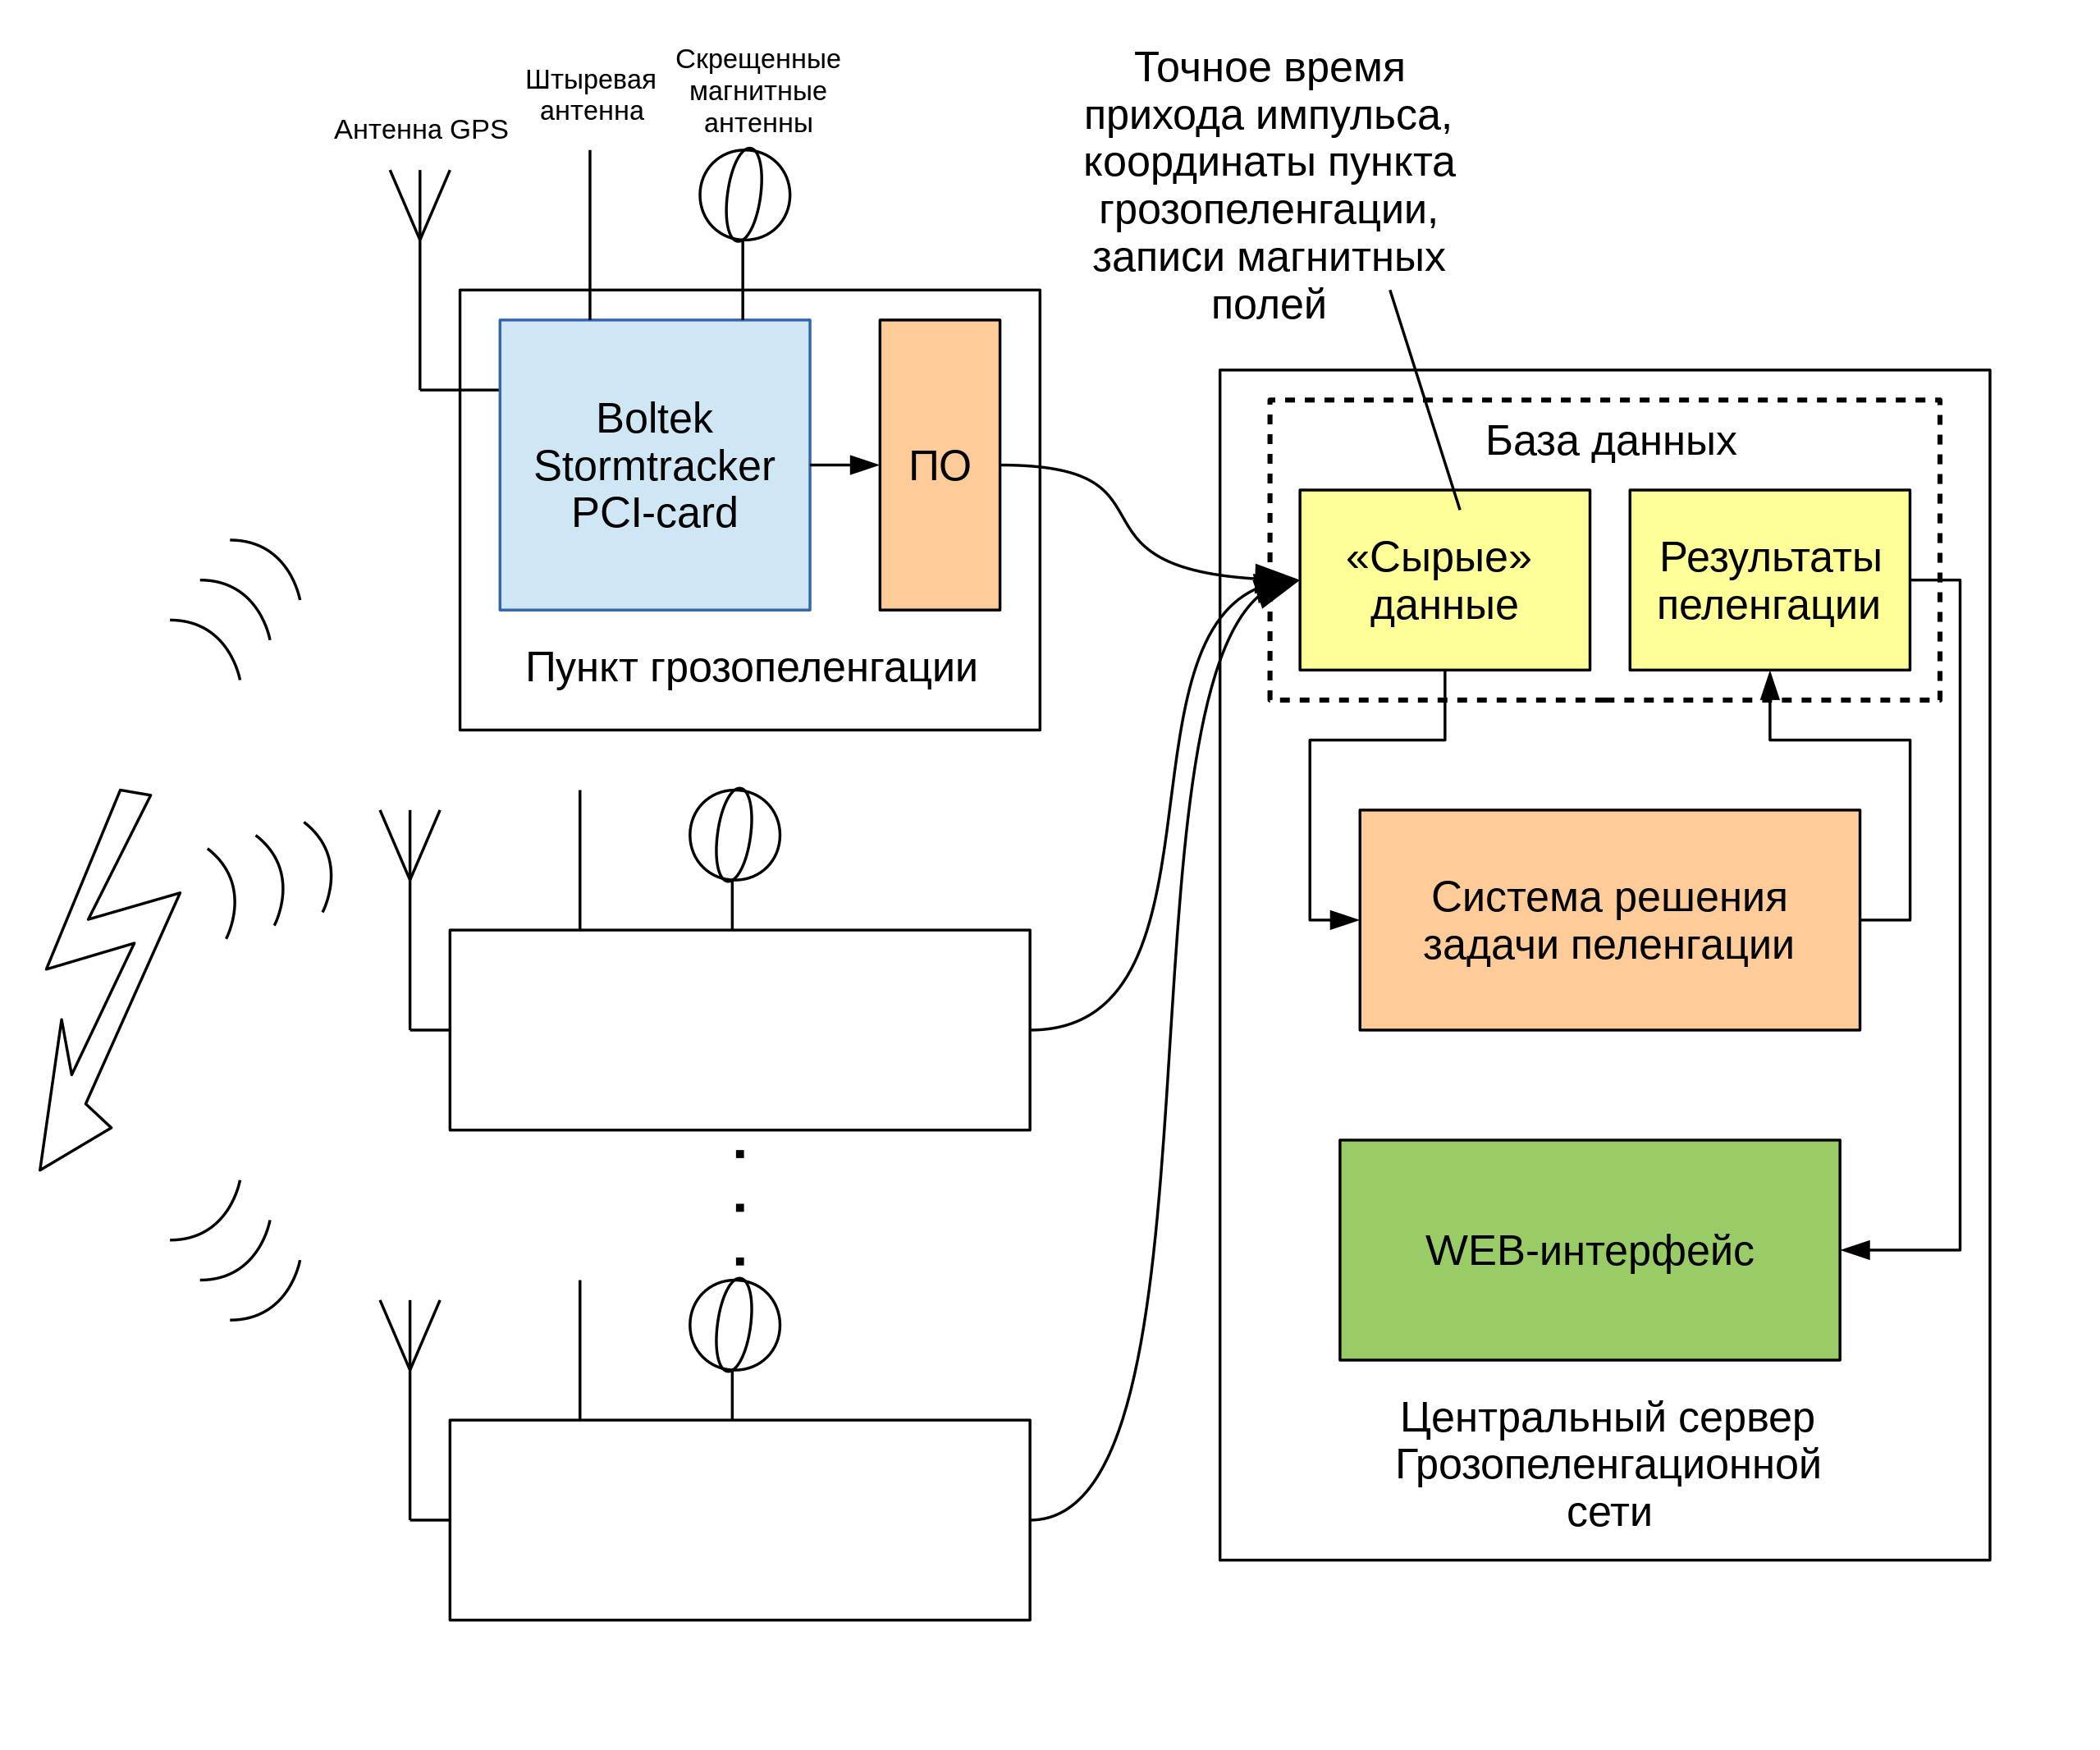
\includegraphics[width=\linewidth]{lds-schematic.png}}
	\caption{Организация грозопеленгационной системы}
	\label{fig:lds-schematic}
\end{figure}

Пункт грозопеленгации включает в себя персональный компьютер, оснащенный PCI-картой Boltek Stormtracker и модулем расширения Boltek LTS2. К PCI-карте подключены антенное устройство в виде двух скрещенных магнитных антенн, принимающих ортогональные горизонтальные компоненты магнитного поля и штыревой электрической антенны, а также GPS-модуль для точного измерения времени прихода электромагнитного импульса, создаваемого молнией. Компьютер оснащен специально разработанным программным обеспечением, работающим под операционной системой GNU/Linux, обеспечивающим сбор, временное хранение и пересылку результатов наблюдения электромагнитных полей на сервер базы данных. Передача данных осуществляется по сети Internet. Технические характеристики пункта грозопеленгаци приведены в таблице~\ref{tab:lds-pars}.

\begin{table}[h]
	\begin{center}
		\begin{tabular}{l|l}
			Характеристика & Значение \\
			\hline
			Частотный диапазон приёмника & $15\ldots100$\,КГц \\
			Частота дискретизации АЦП & 8\,МГц \\
			Разрядность АЦП & 8\,бит \\
			Размер буфера АЦП & 64\,мкс \\
			Минимальный интервал между регистрируемыми событиями & 400\,мкс \\
			Радиус покрытия пункта пеленгации & 400\,км \\
		\end{tabular}	
	\end{center}
	\caption{Характеристики пункта грозопеленгации на основе устройства Boltek Stormtracker}
	\label{tab:lds-pars}
\end{table}

Сервер базы данных грозопеленгационной сети представляет собой компьютер, подключенный к сети Internet, работающий под ОС GNU/Linux. На нём установлено программное обеспечение MariaDB для организации реляционной базы данных (БД) MySQL. База данных содержит в себе всю первичную информацию, поступающую от пунктов грозопеленгации, а также результаты решения задачи пеленгации \cite{rcpl2014}. Данный сервер также содержит веб-интерфейс для доступа к результатам работы системы. Интерфейс ГПС представлен на \figRef{fig:lds-web-interface}.

Решение задачи грозопеленгации происходит на отдельном процессинговом сервере, подключенном к серверу базы данных. Первичные данные загружаются из БД, выделяются пространственно-временные кластеры по алгоритму, описанному в п.\,\ref{sec:space-time-cluster}. Затем, минимизируется функция ошибки. Используемый метод определяется настройками~ПО. Результаты кластеризации, а также точное время и положение молниевого разряда записываются в~БД.

\begin{figure}[h]
	\center{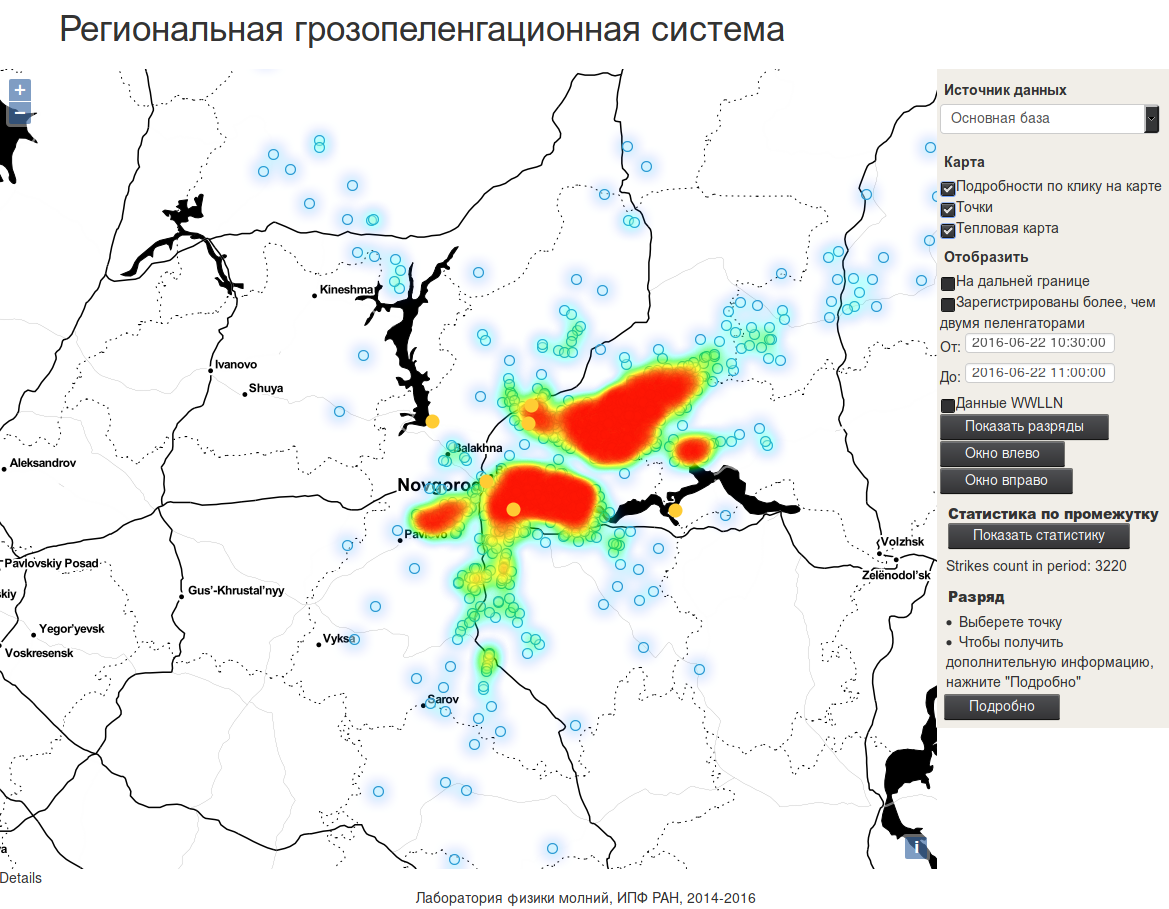
\includegraphics[width=0.9\linewidth]{lds-web-interface.png}}
	\caption{Веб-интерфейс грозопеленгационной системы}
	\label{fig:lds-web-interface}
\end{figure}

Программное обеспечение грозопеленгационной системы разработано в рамках данной работы в соответствии с требованиями к отказоустойчивости, расширяемости и гибкости. При пропадании интернет-соединения между грозопелнегаторами и сервером базы данных информация не теряется, и при восстановлении соединения в целости передаётся в БД. Перемещение пункта пеленгации не требует перенастройки ПО, таким образом системой поддерживаются мобильные грозопеленгаторы. Для добавления нового пункта необходимо лишь добавить одну запись в таблицу конфигурации.

В настоящее время автором данной работы ведётся разработка собственного аппаратного обеспечения для грозопеленгаторов, что позволит существенно снизить стоимость оборудования, габариты приёмников и их энергопотребление. Вследствие этого будет увеличена плотность покрытия~ГПС. В основе будущего грозопеленгатора лежит микроконтроллер STM32F407, подключаемый к одноплатному компьютеру через интерфейс~USB. На данный момент разработаны схемы, встраиваемое программное обеспечение и печатные платы устройства.

\section{Пример работы ГПС}
\label{sec:lds-example}

Для демонстрации возможностей региональный грозопеленгационной системы, как инструмента исследования молниевой активности, рассмотрим грозу 16 июля 2016 г, проходившую на территории Нижегородской области с 14:50 по 16:30 GMT. Она прошла с запада на восток со скоростью в среднем 18 км/ч от г.~Заволжье до ст.~Линда.

\begin{figure}[h]
	\center{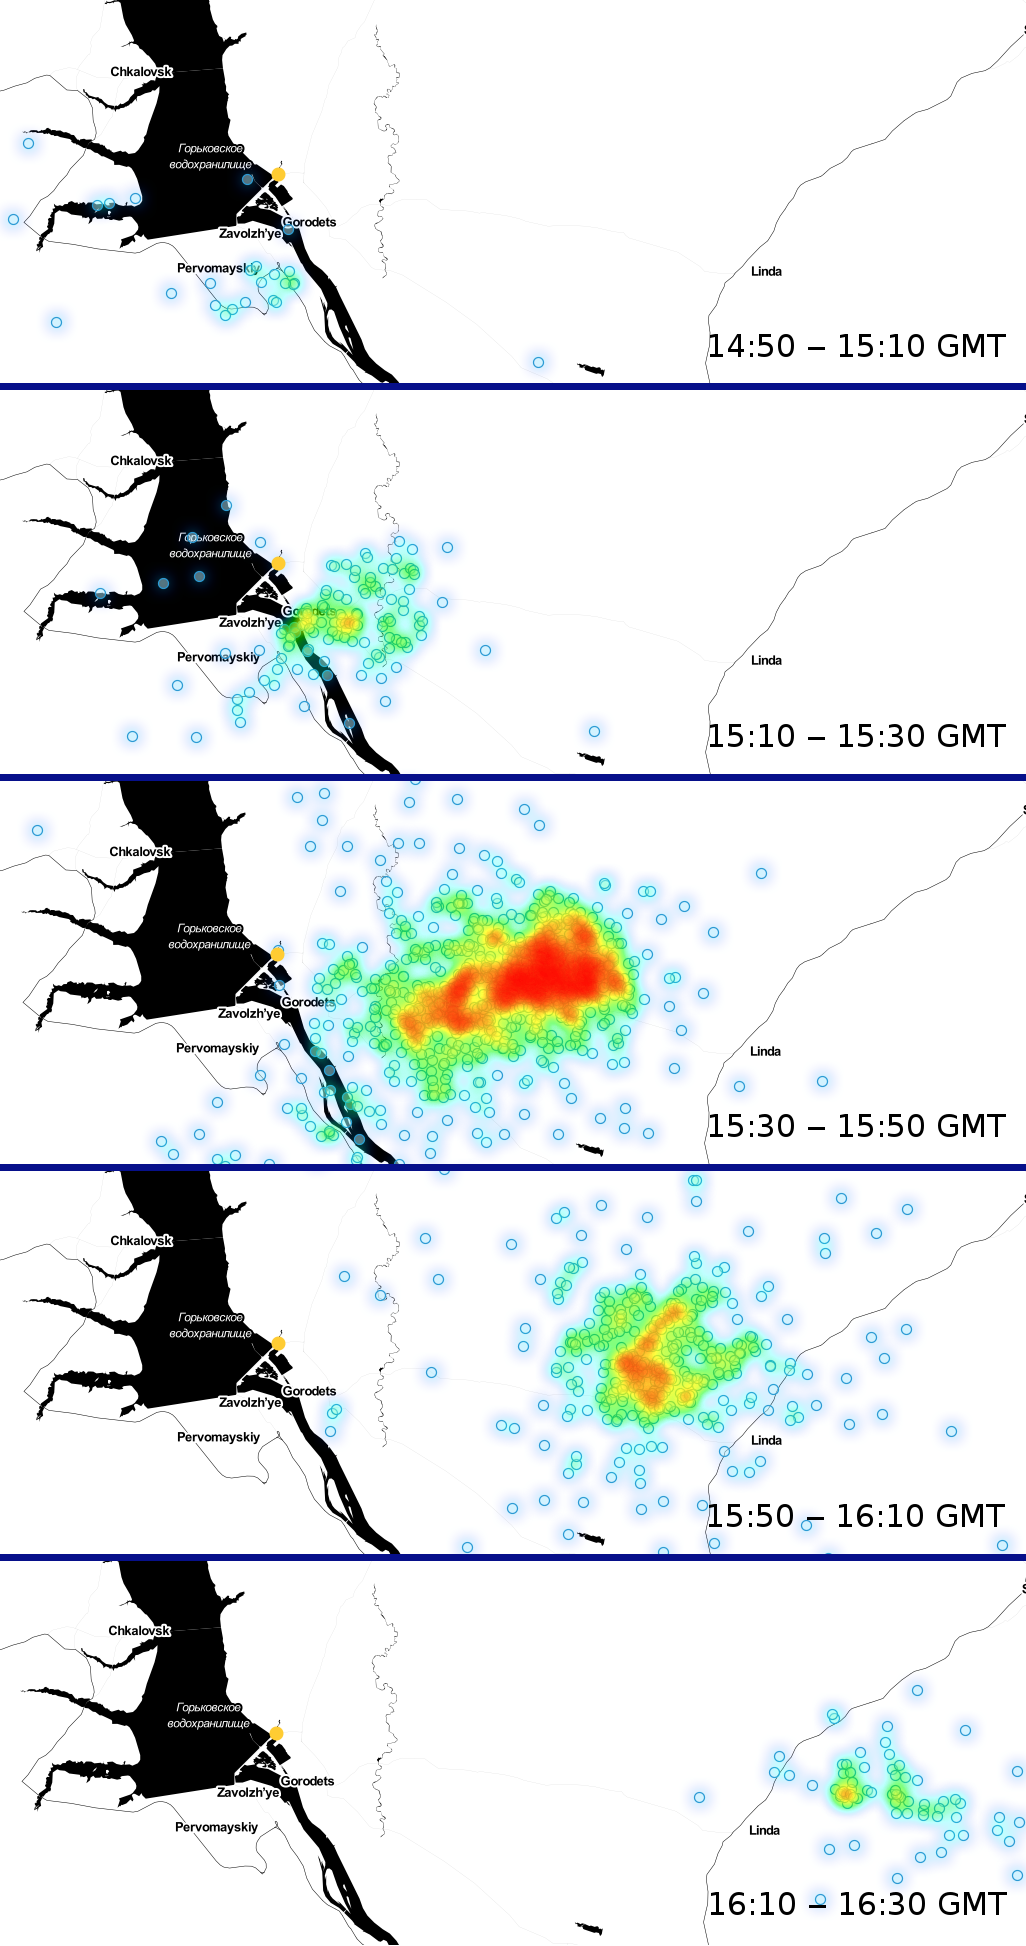
\includegraphics[width=0.45\linewidth]{lds-thunderstorm-move.png}}
	\caption{Визуализация грозы 16 июля 2016}
	\label{fig:lds-thunderstorm-move}
\end{figure}

На \figRef{fig:lds-thunderstorm-move} приведены показания ГПС во временных интервалах 20 мин. Кружками без заливки показаны отдельные молнии, цветом "--- плотность молний на единицу площади в относительных единицах. На \figRef{fig:lds-thunderstorm-freq} показана динамика развития грозы. По вертикали показано количество зарегистрированных молниевых разрядов в минуту. Учитываются как внутриоблачные, так и разряды типа облако-земля. На рисунках хорошо видно возникновение, развитие и угасание грозы.

Данная гроза унесла жизнь человека, купавшегося в Волге \cite{newsnn2016}. В точном соответствии с временем происшествия Нижегородская ГПС зарегистрировала несколько мощных разрядов типа облако-земля в воду вблизи места купания людей.

\begin{figure}[h]
	\center{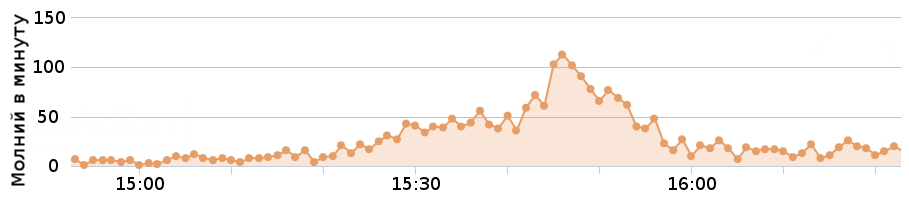
\includegraphics[width=\linewidth]{lds-thunderstorm-freq.png}}
	\caption{Динамика развития грозы 16 июля 2016. По вертикали приведено количество разрядов облако-облако и облако-земля в минуту, включая повторные компоненты}
	\label{fig:lds-thunderstorm-freq}
\end{figure}

\section{Валидация показаний ГПС}
\label{sec:lds-valid}
Важнейшей характеристикой любой грозопеленгационной системы является точность позиционирования разрядов. Этот показатель определяет применимость ГПС для решения тех или иных задач. Определение погрешности ГПС возможно непосредственным образом, либо "--- сравнением с другими системами определения положений молний.

Точные координаты и времена молниевых разрядов могут быть определены по информации, получаемой от молниеотводов, установленных на различных объектах, либо "--- от триггерных молний. Такой подход не применим в текущих условиях. На территории России нет полигонов, оборудованных устройствами для создания триггерных молний. Характерная частота разрядов облако-земля для средней полосы России составляет около 2~разрядов на квадратный километр в год \cite{BaruKononovSolomonic}, поэтому для сбора хотя бы сотни записей за конвективный сезон требуется не менее тысячи автоматических молниеотводов-регистраторов, распределенных по всей области покрытия ГПС.

Альтернативным способом валидации показаний ГПС является сравнение показаний с другими косвенными источниками информации о положении молний. В данной работе использованы данные международной системы WWLLN, а также показания допплеровского метеорадиолокатора (ДМРЛ) \cite{BulatovMiG}.

\begin{figure}[h]
	\center{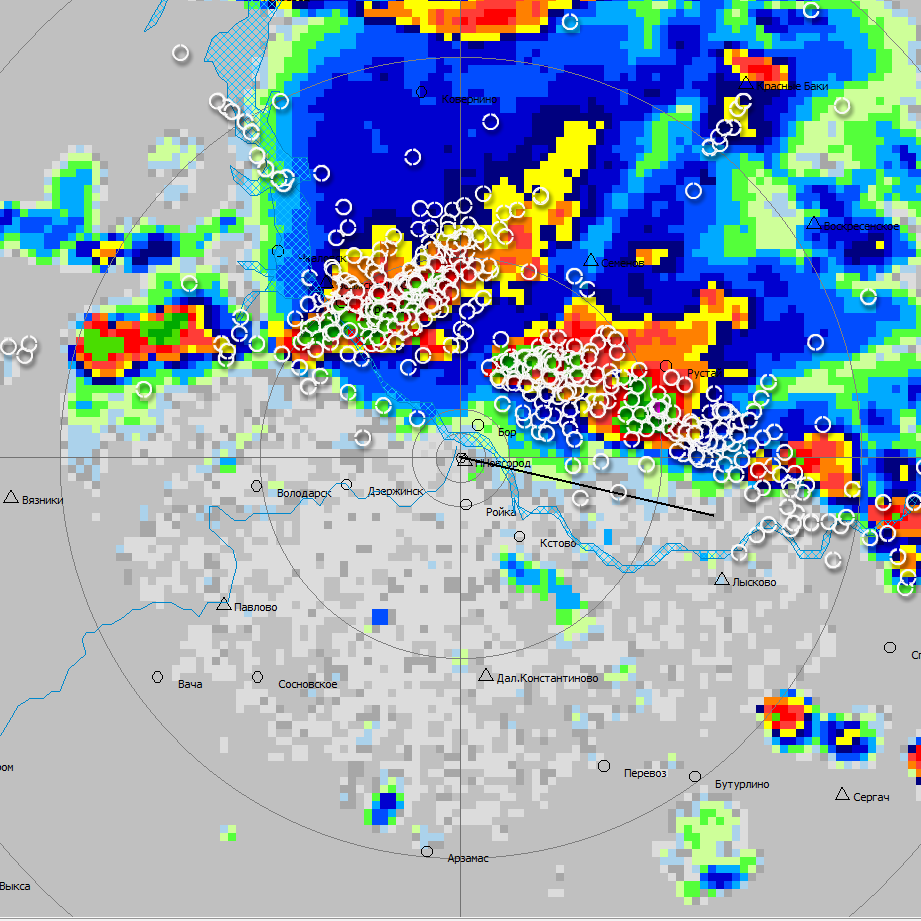
\includegraphics[width=\linewidth]{dmrl-lds.png}}
	\caption{Показания ГПС, наложенные на карту отражаемости ДМРЛ для грозы 5~июля 2015\,г. за промежуток 8:20$\ldots$8:30~GMT}
	\label{fig:dmrl-lds}
\end{figure}

Для качественной проверки точности грозопеленгационной системы проведено сравнение её показаний с данными ДМРЛ. На \figRef{fig:dmrl-lds} приведены отметки ГПС, наложенные на радиолокационную отражаемость облаков, полученную во время грозы 5~июля 2015\,г. за промежуток 8:20$\ldots$8:30~GMT. Наблюдается качественное согласование данных ДМРЛ и показаний системы. Аналогичная согласованность наблюдается для большинства интенсивных гроз конвективных сезонов 2014-2015\,гг. Проведение численного сравнения показаний не представляется возможным, поскольку между радиолокационной отражаемостью и наличием молний имеется лишь косвенная связь \cite{BulatovMiG}.

Точность глобальных систем грозопеленгации, покрывающих большие площади, может варьироваться в зависимости от расстояния до ближайших грозопеленгаторов. Международная глобальная грозопеленгационная система WWLLN покрывает территорию Европейской части России, однако разработчики системы не производили оценку точности её показаний на данной территории. Есть исследования, косвенными методами оценивающие точность WWLLN \cite{Gubenko2014}. В данной работе произведено непосредственное сравнение показаний нижегородской системы и WWLLN, что позволило получить оценки сверху на погрешности обеих систем в силу независимости их ошибок.

При сравнении показаний разработанной грозопеленгационной системы с показаниями следует WWLLN учитывать их особенности. 
Ближайшие грозопеленгаторы WWLLN расположены в Брянске (удаление от Нижнего Новгорода около~700 км), Соданкюле (Лапландия, ок.~1500 км), Ереване (ок.~1800 км) и Будапеште (ок.~2000 км). Грозопеленгаторы нижегородской системы на момент проведения исслдедования точности были расположены в Н. Новгороде, г. Городце и г. Семенове, образуя приблизительно равносторонний треугольник со стороной 60 км. Применение разных методов позиционирования разрядов, а также существенное пространственное удаление пеленгаторов двух систем друг от друга позволяют считать их ошибки независимыми случайными величинами.

\begin{table}[h]
	\begin{center}
		\begin{tabular}{l|l}
			Характеристика & Значение \\
			\hline
			Среднее отклонение по широте $\delta_{lat}$ & 1680\,м \\
			Среднее отклонение по долготе $\delta_{lon}$ & -1780\,м \\
			Стандартное отклонение по широте $\sigma_{lat}$ & 2700\,м \\
			Стандартное отклонение по долготе $\sigma_{lon}$ & 3080\,м \\
		\end{tabular}	
	\end{center}
	\caption{Различие показаний WWLLN и нижегородской ГПС}
	\label{tab:err-pars}
\end{table}

\begin{figure}[h]
	\center{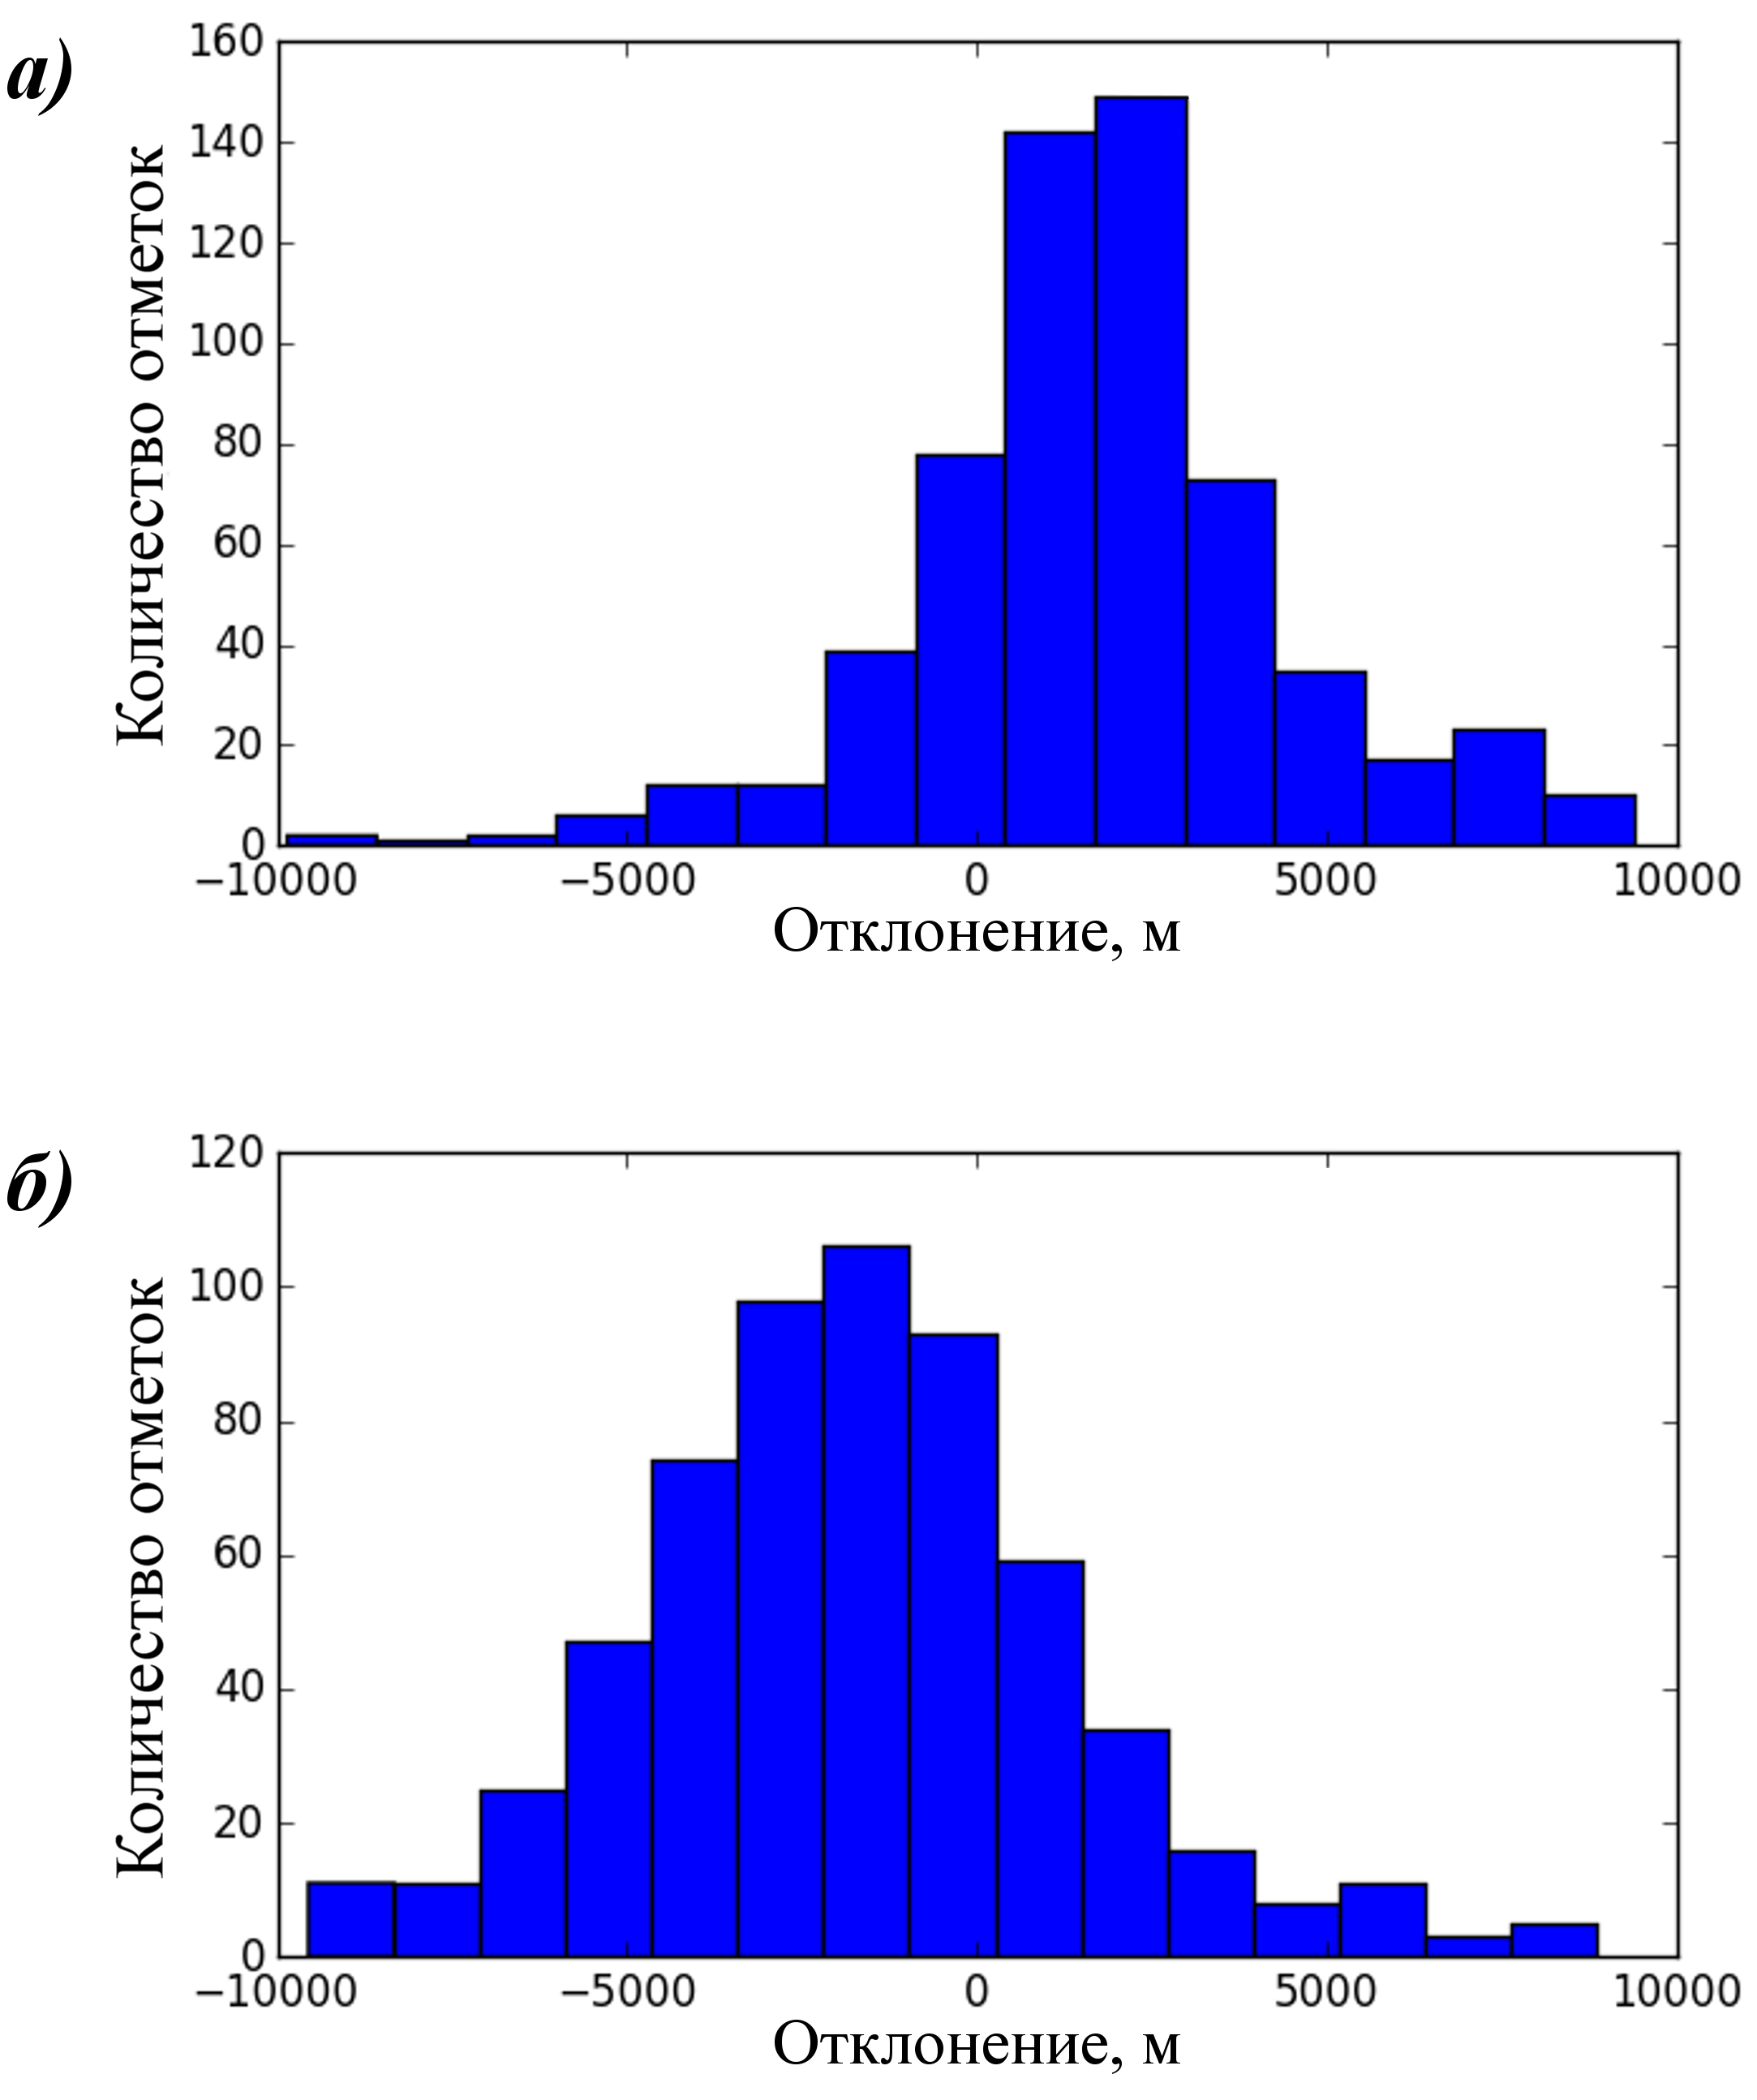
\includegraphics[width=0.5\linewidth]{lds-wwlln-diff.png}}
	\caption{Распределение различия показаний WWLLN и нижегородской ГПС по широте (а) и долготе (б)}
	\label{fig:lds-wwlln-diff}
\end{figure}

Обозначим ошибки WWLLN и нижегородской сети по широте и долготе соответственно за $\Delta_{lat}^{WWLLN}$, $\Delta_{lon}^{WWLLN}$, $\Delta_{lat}^{\text{Ниж}}$, $\Delta_{lon}^{\text{Ниж}}$. Обозначим различие показаний двух систем для одной и той же молниевой вспышки за $\Omega_{lat}$ и $\Omega_{lon}$ соответственно. Тогда, в силу независимости ошибок, для среднего значения $\delta_{lat}$, $\delta_{lon}$ и стандартного отклонения $\sigma_{lat}$, $\sigma_{lon}$ величин $\Omega_{lat}$ и $\Omega_{lon}$ справедливо:
\begin{equation}
	\begin{gathered}
		\delta_{lat, lon} = \overline{\Omega_{lat,lon}} = \overline {\Delta_{lat,lon}^{WWLLN}} + \overline {\Delta_{lat,lon}^{\text{Ниж}}}\\
		\sigma_{lat, lon} = \sigma(\Omega_{lat,lon}) = \sigma (\Delta_{lat,lon}^{WWLLN}) + \sigma (\Delta_{lat,lon}^{\text{Ниж}})
	\end{gathered}
\end{equation}
Таким образом, стандартное отклонение разности показаний может рассматриваться, как оценка сверху для стандартного отклонения ошибок каждой из систем на территории Нижегородской области.

Среди всех молниевых вспышек, отмеченных WWLLN за сезон 2014\,г., были выбраны точки, лежащие в области уверенного приёма нижегородской сети на расстоянии не более 150\,км от ближайшего пеленгатора. Затем отметкам молний WWLLN были поставлены в соответствие отметки, полученные нижегородской системой. Условием соответствия являлось 6различие моментов фиксации по времени не более, чем на $10^{-3}$\,с. Затем определялось различие положений отметок WWLLN и нижегородской сети по широте и долготе. После удаления выбросов, были определены параметры ошибок, приведённые в таблице \ref{tab:err-pars}. При этом было обработано 384 пар отметок WWLLN и нижегородской системы. На \figRef{fig:lds-wwlln-diff} приведены гистограммы отклонения значений нижегородской системы от WWLLN.

Величины  $\delta_{lat}$ и $\delta_{lon}$, вероятнее всего, объясняются систематической погрешностью WWLLN на территории Нижегородской области. Разностно-дальномерный метод, применяемый нижегородской системой, предварительная калибровка оборудования, а также симметрия исследуемой области относительно пеленгаторов исключают возникновение систематической ошибки по одной из координат. В то время как ближайшие приёмники WWLLN расположены в основном западнее исследуемой области, чем может быть объяснено соотношение между $\sigma_{lon}$ и $\sigma_{lat}$.

Таким образом, систематическая ошибка WWLLN на территории Нижегородской может быть оценена приблизительно, как 1780 м на юг и 1680 м на восток при стандартном отклонении 3 км. Стандартное отклонение нижегородской системы также может быть оценено сверху в 3 км. Данные величины могут быть уточнены в меньшую сторону в ходе дальнейших исследований.

\chapter{Исследование молниевой активности по данным ГПС}
Грозопеленгационные системы "--- эффективный инструмент исследования статистических характеристик молниевой активности. Основным вопросом климатологии молний является определение закономерностей поражаемости молниями территорий различных типов. В данной работе исследована зависимость количества гроз от рельефа и степени урбанизации местности. Показано наличие т.\,н. <<урбан-эффекта>> на территории Нижнего Новгорода. Выдвинута гипотеза об отрицательном влиянии мощных ТЭЦ на вероятность возникновения, либо прохождения грозы \cite{BulatovEnergetik2017}. 

По данным ГПС OpenLDS исследованы статистические характеристики повторных компонент обратных ударов на основе более, чем 1,5\,млн. зарегистрированных молний. Показано, что с ростом количества повторных компонент условная вероятность возникновения каждой следующей сначала увеличивается, а затем остаётся постоянной. Получена статистика временных интервалов между повторными компонентами молний, выявлены закономерности.

\section{Особенности распределения молний на территории Нижегородской области}
\label{sec:lds-distr}
Интенсивность молниевой активности на той или иной территории существенно зависит от различных факторов, таких, как тип и рельеф местности, удаленность от крупных водных ресурсов, интенсивность деятельности человека. Характеристиками, непосредственно влияющими на образование грозовых облаков и молний являются концентрация аэрозолей и аэроионов в воздухе, характерная температура и теплоемкость местности, средняя влажность, ветровые характеристики. Одним из проявлений неоднородности распределения молний является т. н. урбан-эффект: согласно некоторым исследованиям, молниевая активность над крупными городами существенно выше, чем над неурбанизированной местностью \cite{Farias2009,Farias2014,Pinto2004}. В работе \cite{BulatovMiG} подтверждено наличие урбан-эффекта на территории Нижнего Новгорода по сравнению с другими участками области.

Для определения интенсивности молниевой активности возможно применение различных показателей: общее количество молниевых разрядов, количество разрядов облако-земля, количество гроз в течение конвективного сезона, суммарный заряд, переносимый молниями в землю и т.п. В работе \cite{BulatovMiG} в качестве основного параметра рассматривается общее количество молниевых разрядов на единицу площади. Такой параметр характеризует грозоопасность местности. Однако важное значение для хозяйственной деятельности и эксплуатации энергетических систем также имеет общее количество гроз в течение конвективного сезона.

В данной работе грозопеленгационной определено системы для количество нескольких гроз участков по данным местности нижегородской на территории Нижегородской области. Под грозой понимается молниевая активность не менее чем 10 разрядов в минуту в радиусе 5 км от опорной точки. Две грозы считаются различными, если в промежутке между ними как минимум в течение часа не зарегистрировано ни одной молнии над исследуемой областью. В качестве опорных точек выбраны следующие:
\begin{enumerate}
	\item Нижний Новгород (56.327\textdegree\,с.\,ш.; 44.003\textdegree\,в.\,д.) "--- мегаполис с населением 1,2~млн.~человек.
	\item Ковернино (57.125\textdegree\,с.\,ш.; 43.812\textdegree\,в.\,д.) "--- поселок городского типа с населением ок.
	7000 человек, сельская местность. Не более 50\% окрестной территории занято	лесом, остальное "--- сельскохозяйственные угодия, вырубки, пастбища и молодые посадки леса.
	\item Керженский биосферный заповедник (56.548\textdegree\,с.\,ш.; 44.923\textdegree\,в.\,д.) "--- практически
	сплошной лес, урбанизация отсутствует.
	\item Заволжье (56.645\textdegree\,с.\,ш.; 43.392\textdegree\,в.\,д.) "--- город на берегу Горьковского водохранилища в непосредственной близости от г.~Городец. Суммарная численность населения обоих городов около 70~тыс.~человек. На территории г.~Заволжье находится обширная инфраструктура Нижегородской ГЭС, состоящая из открытых электрораспределительных устройств, в том числе для ЛЭП напряжением 220 кВ и 110 кВ.
	\item Балахна (56.480\textdegree\,с.\,ш.; 43.540\textdegree\,в.\,д.) "--- город на правом берегу Волги с численностью населения 50~тыс.~человек. В Балахне находится Нижегородская ГРЭС им. А.\,В.~Винтера с установленной электрической мощностью 144\,МВт и тепловой 566\,Гкал/час.
	\item Кстово (56.151\textdegree\,с.\,ш.; 44,195\textdegree\,в.\,д.) "--- город с населением 67~тыс.~человек. В Кстово
	располагается Новогорьковская ТЭЦ с установленной электрической мощностью
	548,3 МВт и тепловой 626 Гкал/час.
\end{enumerate}

Помимо прочих факторов, выбранные области позволяют исследовать влияние объектов энергетической инфраструктуры на вероятность возникновения гроз.

\begin{figure}[h]
	\center{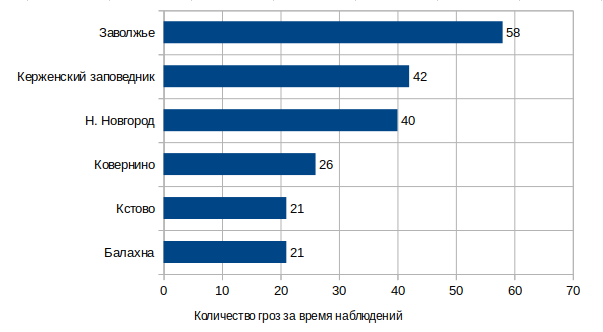
\includegraphics[width=0.8\linewidth]{lds-places-stat.png}}
	\caption{Количество гроз над исследуемыми территориями, зарегистрированных за период с июля 2014\,г. по август 2016\,г.}
	\label{fig:lds-places-stat}
\end{figure}

Для данных участков за промежуток с июля 2014\,г. по август 2016\,г. определено суммарное количество гроз. Результаты приведены на \figRef{fig:lds-places-stat}. Только около 15\% гроз покрывали одновременно все исследуемые территории, в большинстве случаев они имели более локальный характер. В целом, для исследованных регионов характерна существенная неоднородность вероятности прохождения гроз с различием для отдельных областей более, чем в 2,7~раза, что говорит о наличии существенных механизмов, влияющих на грозовую активность.

Для объяснения существенного различия в количестве гроз были предложены некоторые гипотезы. Из диаграммы видно, что наибольшее количество гроз характерно для г.~Заволжье. В качестве возможного объяснения высоких показателей можно привести сочетание двух факторов: нахождение на берегу водохранилища и большая площадь электроэнергетической инфраструктуры.

Минимальное количество гроз зарегистрировано в окрестностях городов Балахна и Кстово. В отличие от остальных исследуемых территорий, в обоих городах находятся мощные ТЭЦ. Детальное рассмотрение структуры отдельных гроз в окрестностях Балахны и Кстово средствами нижегородской ГПС также показало, что грозы средней и малой относительной интенсивности как бы огибают данные участки. Заметим, что на ГРЭС в Балахне для охлаждения используется пруд значительной площади, а на Новогорьковской ТЭЦ в Кстово для охлаждения используются градирни Это позволяет выдвинуть гипотезу о влиянии инфраструктуры ТЭЦ на снижение частоты гроз в окрестности. Такой эффект может объясняться большим локальным выбросом тепла, влияющим на развитие грозовых облаков, а также поступлением водяного пара от охлаждающих систем и образующегося в результате сгорания топлива одновременно с образованием углекислого газа. Изучение конкретного механизма воздействия выходит за рамки данной работы и является задачей дальнейших тематических исследований.

В окрестностях Ковернино вероятность гроз также не высока, однако на 23\% превышает такой показатель для Кстово и Балахны. При этом для Ковернино картина в целом совпадает со всем Ковернинским районом, никак не выделяя районный центр, что не справедливо для Кстово и Балахны. Поэтому логичным объяснением снижения частоты гроз может являться отсутствие промышленности, низкая численность населения и относительно малое количество леса.

Другим интересным результатом является приблизительно одинаковый уровень грозовой активности для двух совершенно разных типов местности, удаленных на расстояние порядка 65 км: города-мегаполиса Н. Новгорода и Керженского биосферного заповедника. В обоих случаях наблюдается высокая вероятность гроз, что обусловлено различными факторами. В мегаполисе возможной причиной может являться большое количество аэрозолей, что согласуется с аэрозольной теорией урбан-эффекта \cite{Farias2009}. В случае леса причиной может быть повышенная интенсивность образования аэроионов, отличия в суточном цикле влажности и другие факторы.

\section{Статистические характеристики повторных разрядов}
\label{sec:lds-stat-rep}
Хорошо известно, что главная стадия молнии, <<обратный удар>>, может многократно повторяться. Считается, что примерно половина всех разрядов облако-земля является многократными, причём количество повторений в отдельных случаях может достигать десятков раз \cite{RakovUman2005}. 

Для исследования мультипликативности обратного удара применимы региональные грозопеленгационные системы. В отличие от глобальных, они регистрируют практически 100\% молниевых вспышек в определенной местности. При достаточном временном разрешения такие системы хорошо различают компоненты обратного удара. ГПС~OpenLDS, разработанная в рамках данной работы, позволила исследовать статистические характеристики повторных разрядов на территории Нижегородской и соседних областей.

Для анализа использованы все данные, полученные системой за время функционирования с 2014 по 2017\,гг. За данный период грозопеленгационная система зарегистрировала более~2,2~млн.~молниевых разрядов.

\subsection{Определение повторных компонент молний}
Временное разрешение ГПС OpenLDS позволяет разрешать повторные компоненты молний. Информация, предоставляемая ГПС, представляет собой координаты, широту и долготу~$(\theta_i, \varphi_i)$ и время~$t_i$ для каждого разряда. Условием того, что два последовательно зарегистрированных разряда являются компонентами одной молнии, является их географическая близость и достаточно малый промежуток времени между ними. Однако, если промежуток времени слишком мал, это может означать, что ГПС зарегистрировала дважды один и тот же разряд. Таким образом, условием того, что разряд $i+1$ является повтором после разряда $i$ является:
\begin{equation}
	\begin{gathered}
		\rho\left[(\theta_i, \varphi_i), (\theta_{i+1}, \varphi_{i+1})\right] < \rho_{max},\\ \Delta t_{min} < t_{i+1} - t_i < \Delta t_{max}
		\label{eq:criteria}
	\end{gathered}
\end{equation}
где функция $\rho$ "--- расстояние между точками на поверхности Земли.

В качестве величины $\rho_{max}$ в формуле \eqref{eq:criteria} взята погрешность ГПС, 3\,км. В качестве величины $\Delta t_{max}$ "--- максимальной задержки между повторными компонентами, взято 0,4\,с. Такое значение гарантировано превышает средний интервал между компонентами обратного удара \cite{RakovUman2005}. Величина $\Delta t_{min} = 100$\,мкс, что превышает характерную длительность тока обратного удара. Экспериментально установлено, что для величины $\Delta t_{min} \in [5\text{\,мкс}, 500\text{\,мкс}]$ результаты статистической обработки данных не меняются, что позволяет сделать вывод о практически полном отсутствии случаев двойной регистрации однократного обратного удара с интервалом более 5\,мкс.

Рассмотрим надёжность данного критерия с точки зрения ложноположительного результата. Теоретически, возможно возникновение двух независимых молний на расстоянии, меньшем $\rho_{max}$ через промежуток времени, меньший $\Delta t_{max}$. Однако, по данным ГПС, самые сильные грозы в регионе имеют интенсивность не более 250 разрядов в минуту считая все компоненты и внутриоблачные разряды. Оценивая снизу область такой грозы в $1000\,\text{км}^2$, получаем вероятность ложноположительного обнаружения повторной компоненты~$P_{err}=0,5\%$. Данная оценка справедлива всего для нескольких грозовых часов в году и становится существенно меньше для менее интенсивных гроз. Что касается N-кратных разрядов, вероятность ложноположительного их детектирования равна $P_{err}^N$, что представляет собой исчезающе малую величину для выборки в 2,2~млн~записей.

Особенностью грозопеленгационной системы OpenLDS, на данный момент, является невозможность надёжного различения типа и знака молниевого разряда. Однако, считается, что количество повторных компонент главной стадии молнии более 3 преимущественно характерно для отрицательных разрядов типа облако-земля \cite{RakovUman2005}. Таким образом, основные выводы работы справедливы для отрицательных молний, ударяющих в землю.

\begin{figure}[h]
	\center{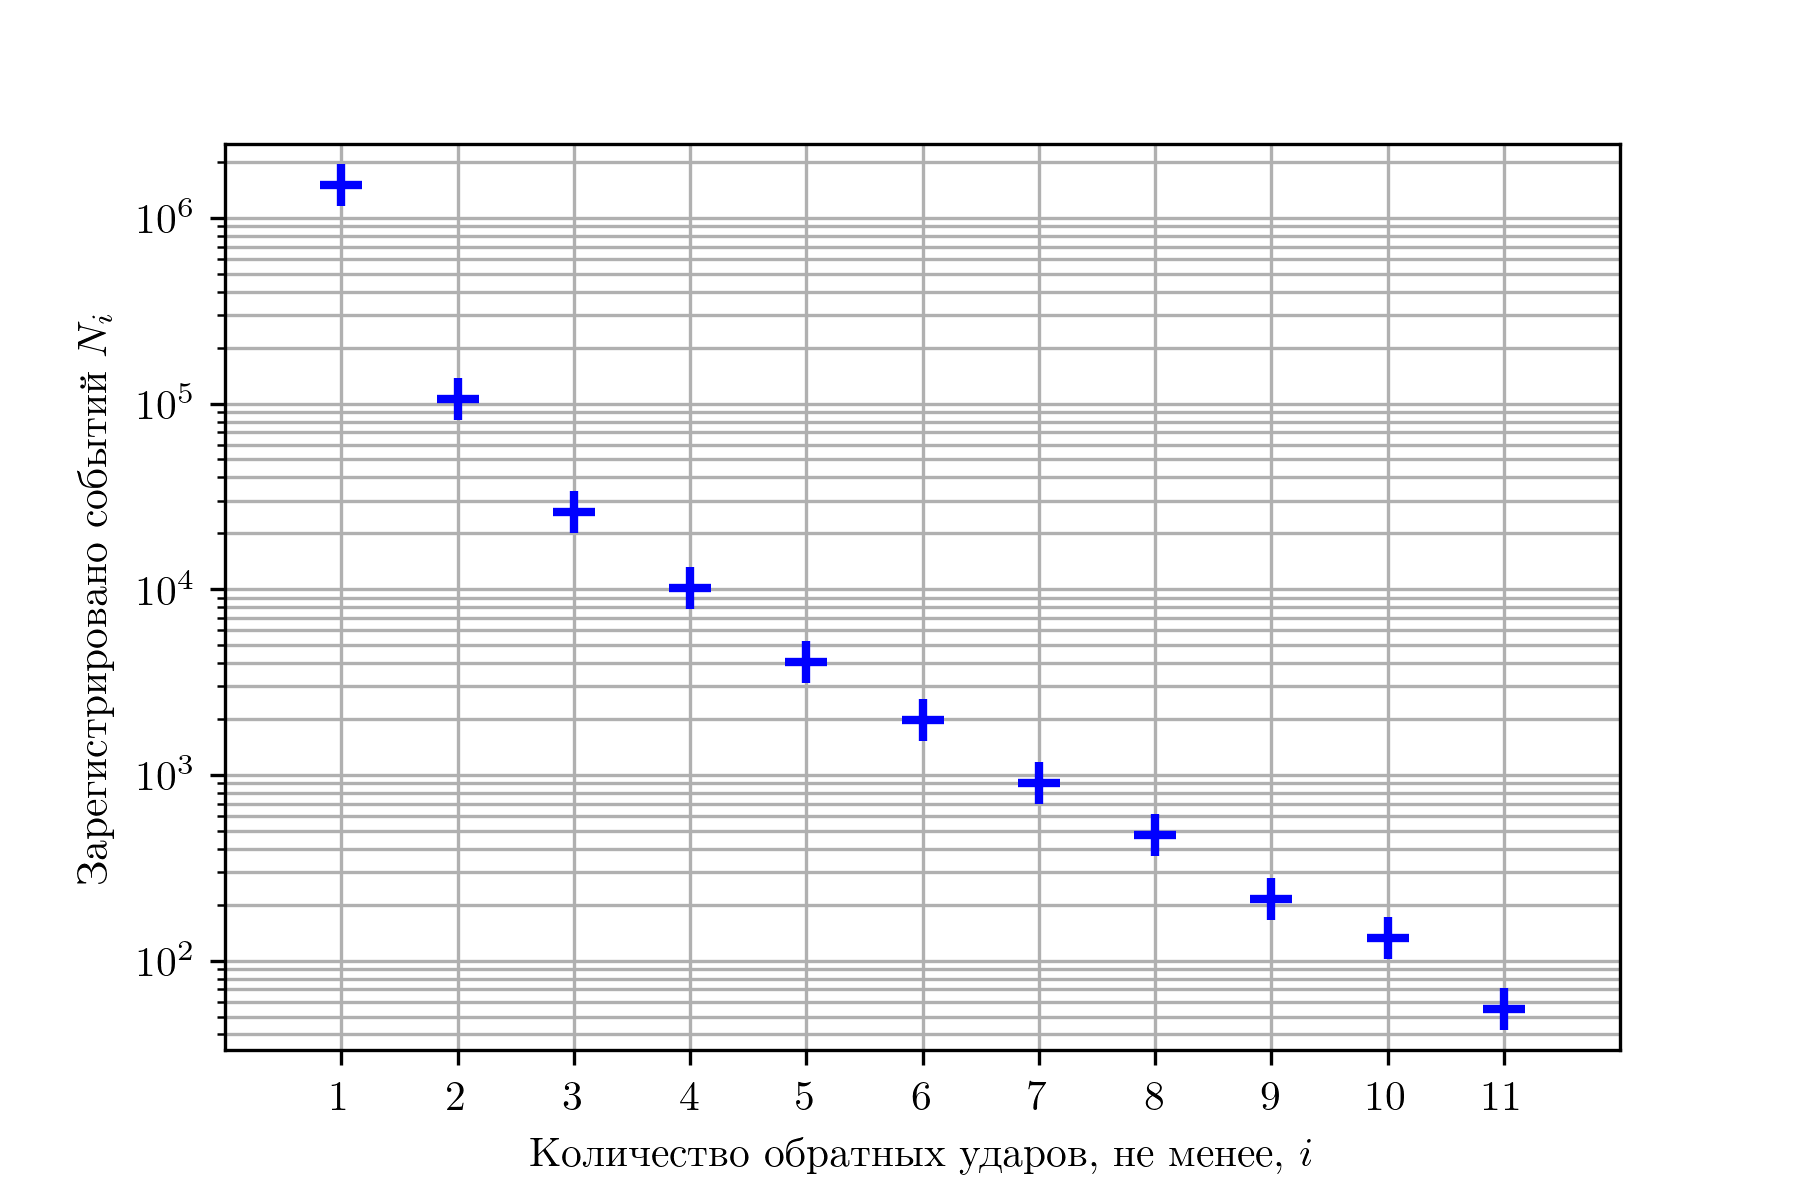
\includegraphics[width=0.9\linewidth]{lds-reps.png}}
	\caption{Количество событий с определенным числом повторов обратного удара}
	\label{fig:lds-reps}
\end{figure}

\subsection{Повторяемость обратного удара}
За время наблюдений зарегистрировано приблизительно 1,5\,млн. молний, 106\,тыс. из которых имели повторные компоненты. В области покрытия ГПС за время наблюдения зарегистрировано до 16 повторов главной компоненты молнии, наблюдалось 3 таких события во время интенсивных гроз в августе 2016\,г.

Рассмотрим статистику количества повторов главной стадии молнии, полученную на основе критерия \eqref{eq:criteria}. На \figRef{fig:lds-reps} приведена зависимость количества зарегистрированых событий $N_i$ от числа повторов обратного удара $i$ в полу-логарифмическом масштабе. Величина $N_i$ включает в себя как случаи, когда обратный удар повторился ровно $i$ раз, так и случаи с $i+1$, $i+2$, $...$ повторениями. Численные значения величины $N_i$ приведены в таблице \ref{tab:lds-intervals}.

\begin{figure}[h]
	\center{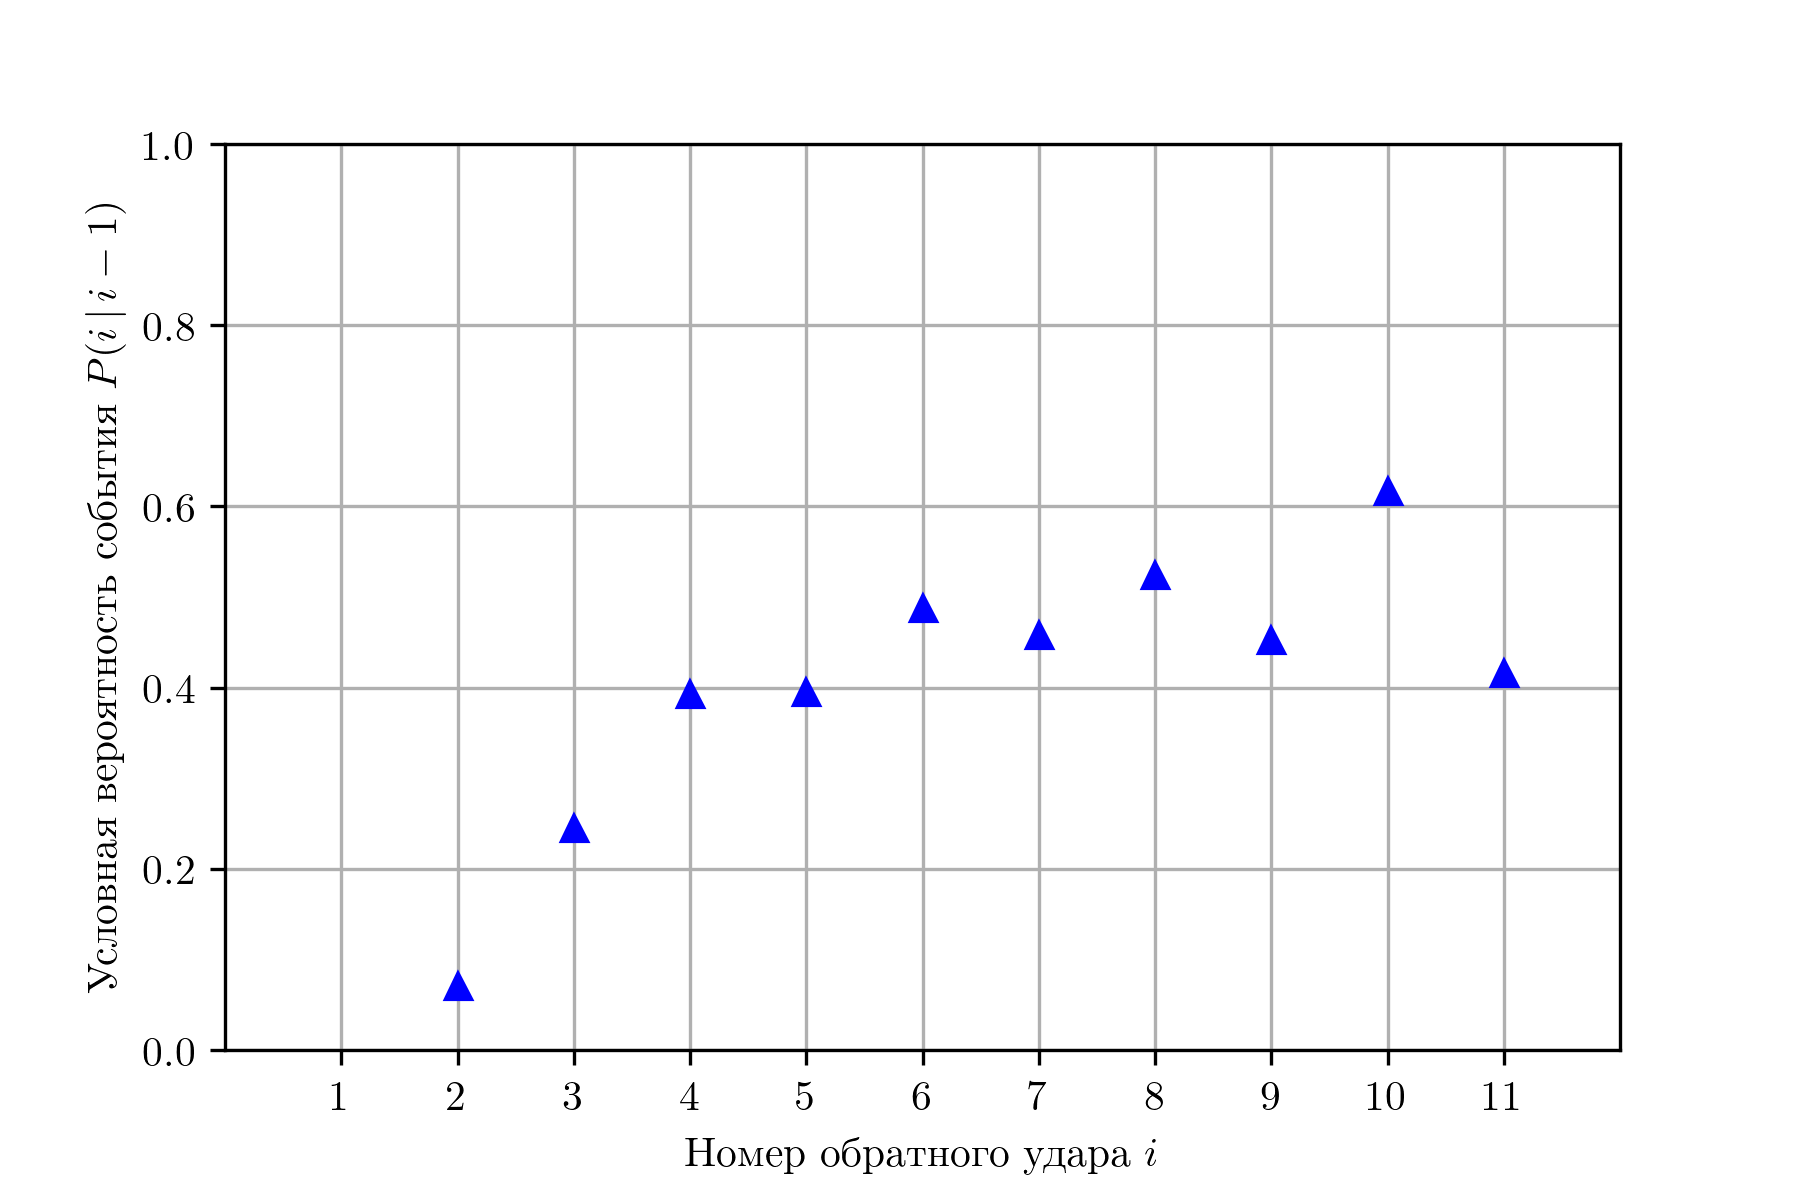
\includegraphics[width=0.9\linewidth]{lds-probs.png}}
	\caption{Условные вероятности возникновения повторных обратных ударов}
	\label{fig:lds-probs}
\end{figure}

Если провести кривую через точки на \figRef{fig:lds-reps}, будет заметна выпуклость кривой вниз. Рассмотрим условную вероятность развития $i$-го повтора обратного удара при условии того, что повтор $i-1$ имел место:
\begin{equation}
	P(i\,|\,i-1) = \frac{N_i}{N_{i-1}}.
\end{equation}
Другими словами, если мы наблюдаем за грозой сразу после того момента, когда произошло $i$ повторов главной стадии молнии, с вроятностью $P(i\,|\,i-1)$ произойдёт и $(i+1)$-ый повтор.

На \figRef{fig:lds-probs} приведена зависимость величины $P(i\,|\,i-1)$ от $i$. Её численные значения приведены в таблице \ref{tab:lds-intervals}. Условная вероятность существенно растёт от 0,24 до 0.52 на интервале от 2 до 8 повторов обратного удара. Далее вероятность достигает насыщения и её колебания обуславливаются уменьшением мощности выборки. 

\subsection{Статистика временных интервалов}

Рассмотрим временные интервалы между компонентами одной молнии. На \figRef{fig:lds-hist} приведены гистограммы интервалов между первым (главным) и вторым обратными ударами, между вторым и третьим, третьем и четвёртым, четвертым и пятым. Распределения нормированы на единицу, графики представляют собой плотности вероятности. В таблице~\ref{tab:lds-intervals} приведены численные значения средних ($\overline {\Delta t_i}$) и медианных ($\Delta t_i^m$) интервалов между разрядами, а также их стандартного отклонения. Эти же данные представлены на графике на \figRef{fig:lds-graph}.

\begin{figure}[h]
	\center{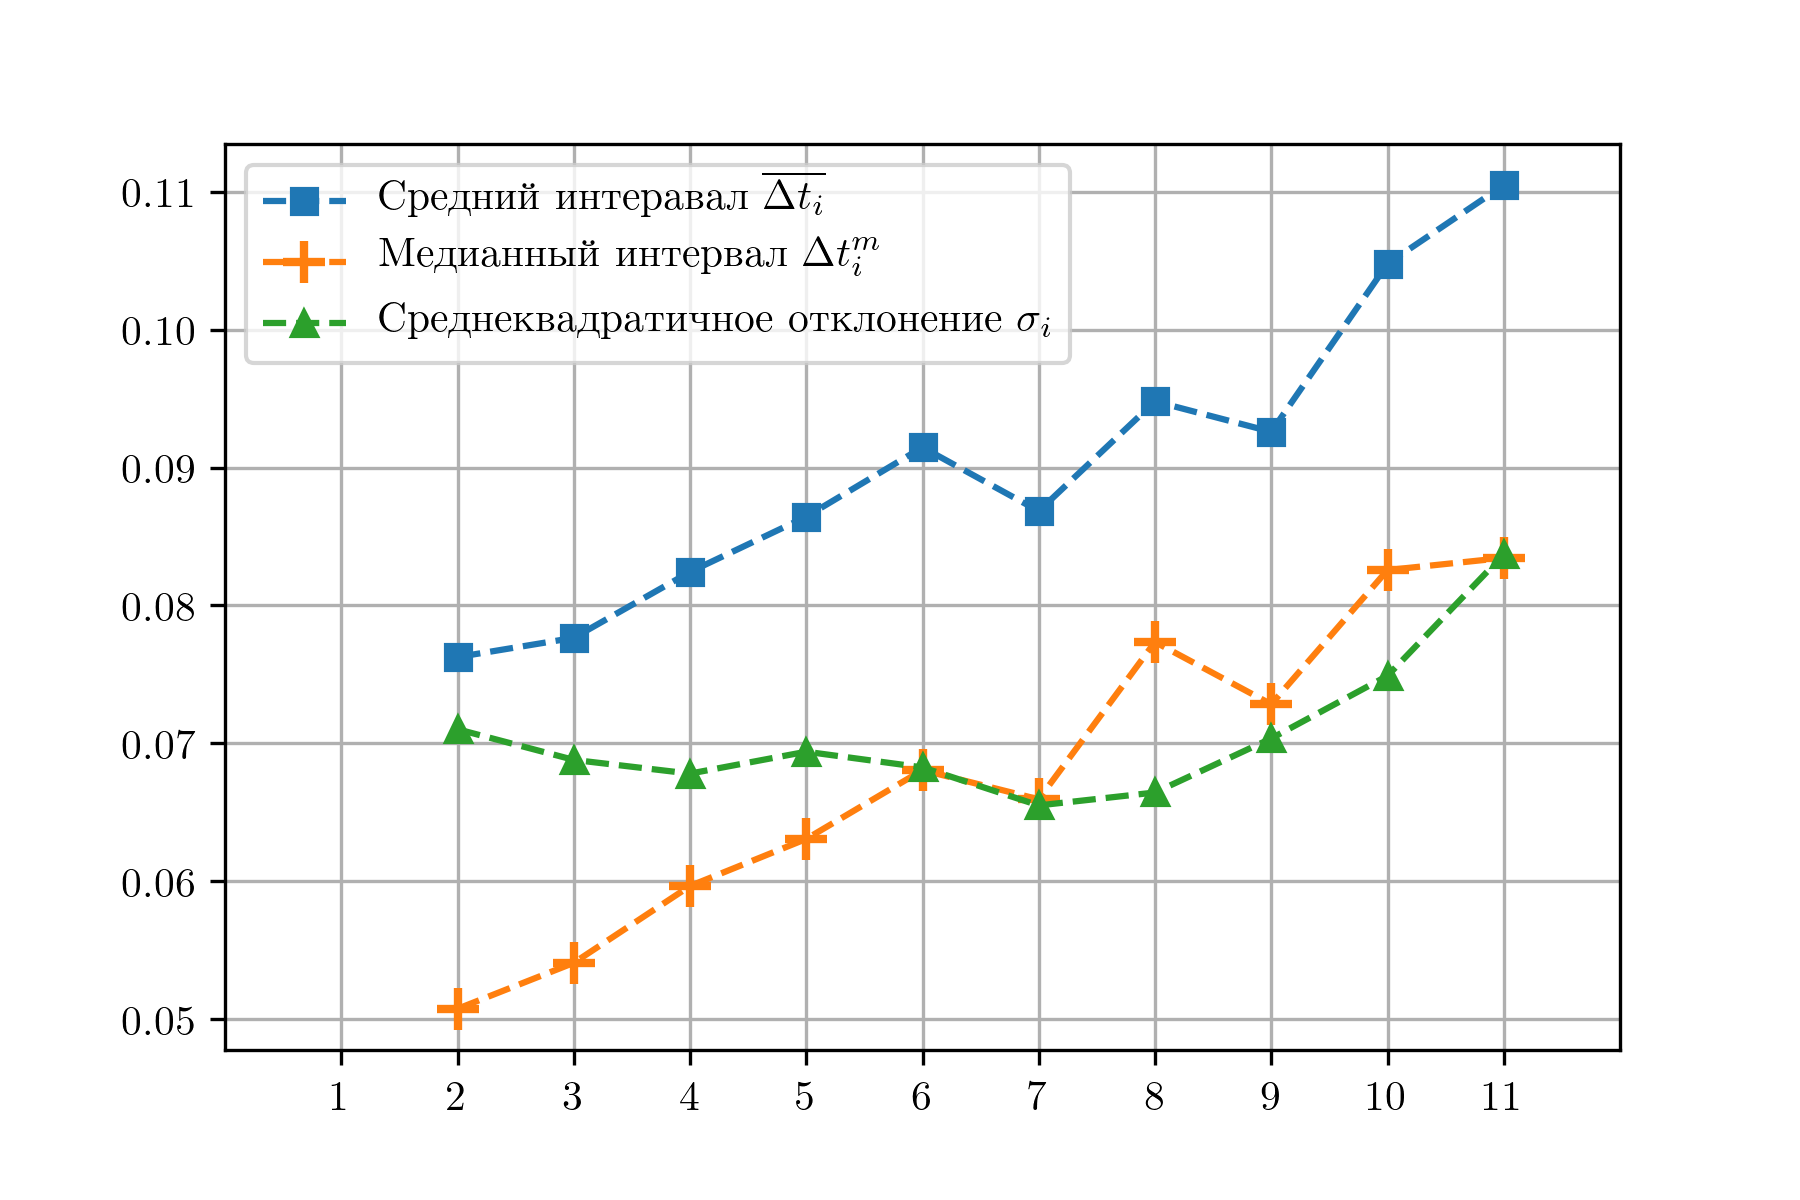
\includegraphics[width=0.9\linewidth]{lds-graphs.png}}
	\caption{Зависимость среднего, медианного значений временного интервала и его стандартного отклонения от номера повтора компоненты разряда}
	\label{fig:lds-graph}
\end{figure}

\begin{table}[h]
	\centering
	\begin{tabular}{ c | c | c | c | c | c }
		%\hline
		
		\begin{sideways} Количество обратных ударов $i$ \end{sideways} &
		\begin{sideways} Количество событий $N_i$ \end{sideways} &
		\begin{sideways} Условная вероятность $P(i\,|\,i-1)$ \end{sideways} &
		\begin{sideways} Средний интервал $\overline {\Delta t_i}$, мс \end{sideways} &
		\begin{sideways} Медианный интервал $\Delta t_i^m$, мс \end{sideways} &
		\begin{sideways} Стандартное отклонение $\sigma_i$, мс \end{sideways} \\ \hline
		\rule{0pt}{14pt} 1 & 1394457 & -- & -- & -- & -- \\
		\rule{0pt}{14pt} 2 & 80280 & 0.07 & 76 & 50 & 71 \\
		\rule{0pt}{14pt} 3 & 15765 & 0.24 & 77 & 54 & 69 \\
		\rule{0pt}{14pt} 4 & 6180  & 0.39 & 82 & 60 & 68 \\
		\rule{0pt}{14pt} 5 & 2065  & 0.40 & 86 & 63 & 69 \\
		\rule{0pt}{14pt} 6 & 1068  & 0.49 & 91 & 68 & 68 \\ 
		\rule{0pt}{14pt} 7 & 429   & 0.46 & 87 & 66 & 65 \\ 
		\rule{0pt}{14pt} 8 & 259   & 0.52 & 95 & 77 & 66 \\ 
		\rule{0pt}{14pt} 9 & 82    & 0.45 & 93 & 73 & 70 \\ 
		\rule{0pt}{14pt} 10 & 77   & 0.61 & 105 & 83 & 74 \\ 
		\rule{0pt}{14pt} 11 & 19   & 0.41 & 110 & 83 & 83 \\ 
	\end{tabular}
	\caption{Статистические характеристики интервалов между повторными разрядами}
	\label{tab:lds-intervals}
\end{table}

\subsection{Обсуждение результатов}
Рост и насыщение величины $P(i\,|\,i-1)$ имеет существенное значение и является одним из главных результатов исследования (см. \figRef{fig:lds-probs}). Рассмотрим факторы, которые могут прервать последовательность повторений обратного удара для среднестатистической отрицательной молнии: деградацию молниевого канала и истощение заряда облака.

Известно, что при наличии повторных компонент большая часть молниевого канала <<переиспользуется>> этими компонентами \cite{Rakov-PhysicsOfLightning}. В промежутках между вспышками канал может деградировать: остывать, рекомбинировать и разрушаться под действием порывов ветра и других факторов. Процесс деградации происходит по определенным законам и время разрушения канала зависит от его начальных характеристик. После прохождения разряда канал <<обновляется>>, и процесс распада начинается заново. При распаде канала до некоторого критического состояния дальнейшее повторение обратных ударов становится невозможным.

%<<Качество канала>> определяется, в первую очередь, температурой нейтрального газа и остаточной ионизацией, а также пространственным распределением этих параметров. Однако, для упрощения, <<качество>> можно параметризовать в виде некоторой переменной $Q$. Тогда, вероятность развития повторной компоненты определяется величиной $Q$ и доступностью необходимого для стреловидного лидера заряда. С течением времени происходит уменьшение величины $Q(t+\Delta t) = Q(t)\cdot \exp(-\alpha t)$. С каждым разрядом~$Q$ мгновенно увеличивается на некоторую величину $\Delta Q$. Если интервал между разрядами составляет $\Delta е$, то в зависимости от соотношения $\alpha$, $\Delta Q$ и $\Delta t$ среднее значение качества канала может как падать, так и расти.

Другим фактором, влияющим на возможность развития разряда, являться истощение заряда в досягаемой части облака. Транспортная система, собирающая заряд, имеет ограниченные возможности прорастания вглубь облака и конечную скорость сбора нового заряда. Количество доступного заряда может быть в принципе ограниченным.

Согласно экспериментальным данным, полученным в рамках исследования, показано, что средний интервал $\overline {\Delta t_i}$ между повторными компонентами монотонно увеличивается от 76 до 110\,мс (\figRef{fig:lds-graph}). Это подтверждает замедление процесса сбора заряда. Однако, если бы доступный для среднестатистической молнии заряд мог бы быть исчерпан одной многокомпонентной молнией, наблюдалось бы уменьшение условной вероятности развития новой компоненты начиная с некоторого характерного числа повторов. Другими словами, одна многокомпонентная молния не способна разрядить облако на масштабах её транспортной системы.

<<Качество канала>> определяется, в первую очередь, температурой нейтрального газа и остаточной ионизацией, а также пространственным распределением этих параметров. В рамках данного подхода, рост и насыщение величины $P(i\,|\,i-1)$ объясняется следующим образом: когда средний интервал между молниями $\overline {\Delta t_i}$ мал, каждая следующая компонента дополнительно прогревает канал и генерирует ионы. Этот эффект накапливается и повышает вероятность последующих компонент. Однако, когда $\overline {\Delta t_i}$ увеличивается из-за растущих трудностей при сборе заряда, растёт также и время деградации канала между разрядами, и процесс деградации уравновешивает нагрев и ионизацию при разрядах. В дальнейшем, с ростом $i$, деградация начнёт доминировать и условная вероятность будет снижаться. Однако такой эффект не наблюдается при значениях $i \le 12$.

\begin{figure}[h]
	\center{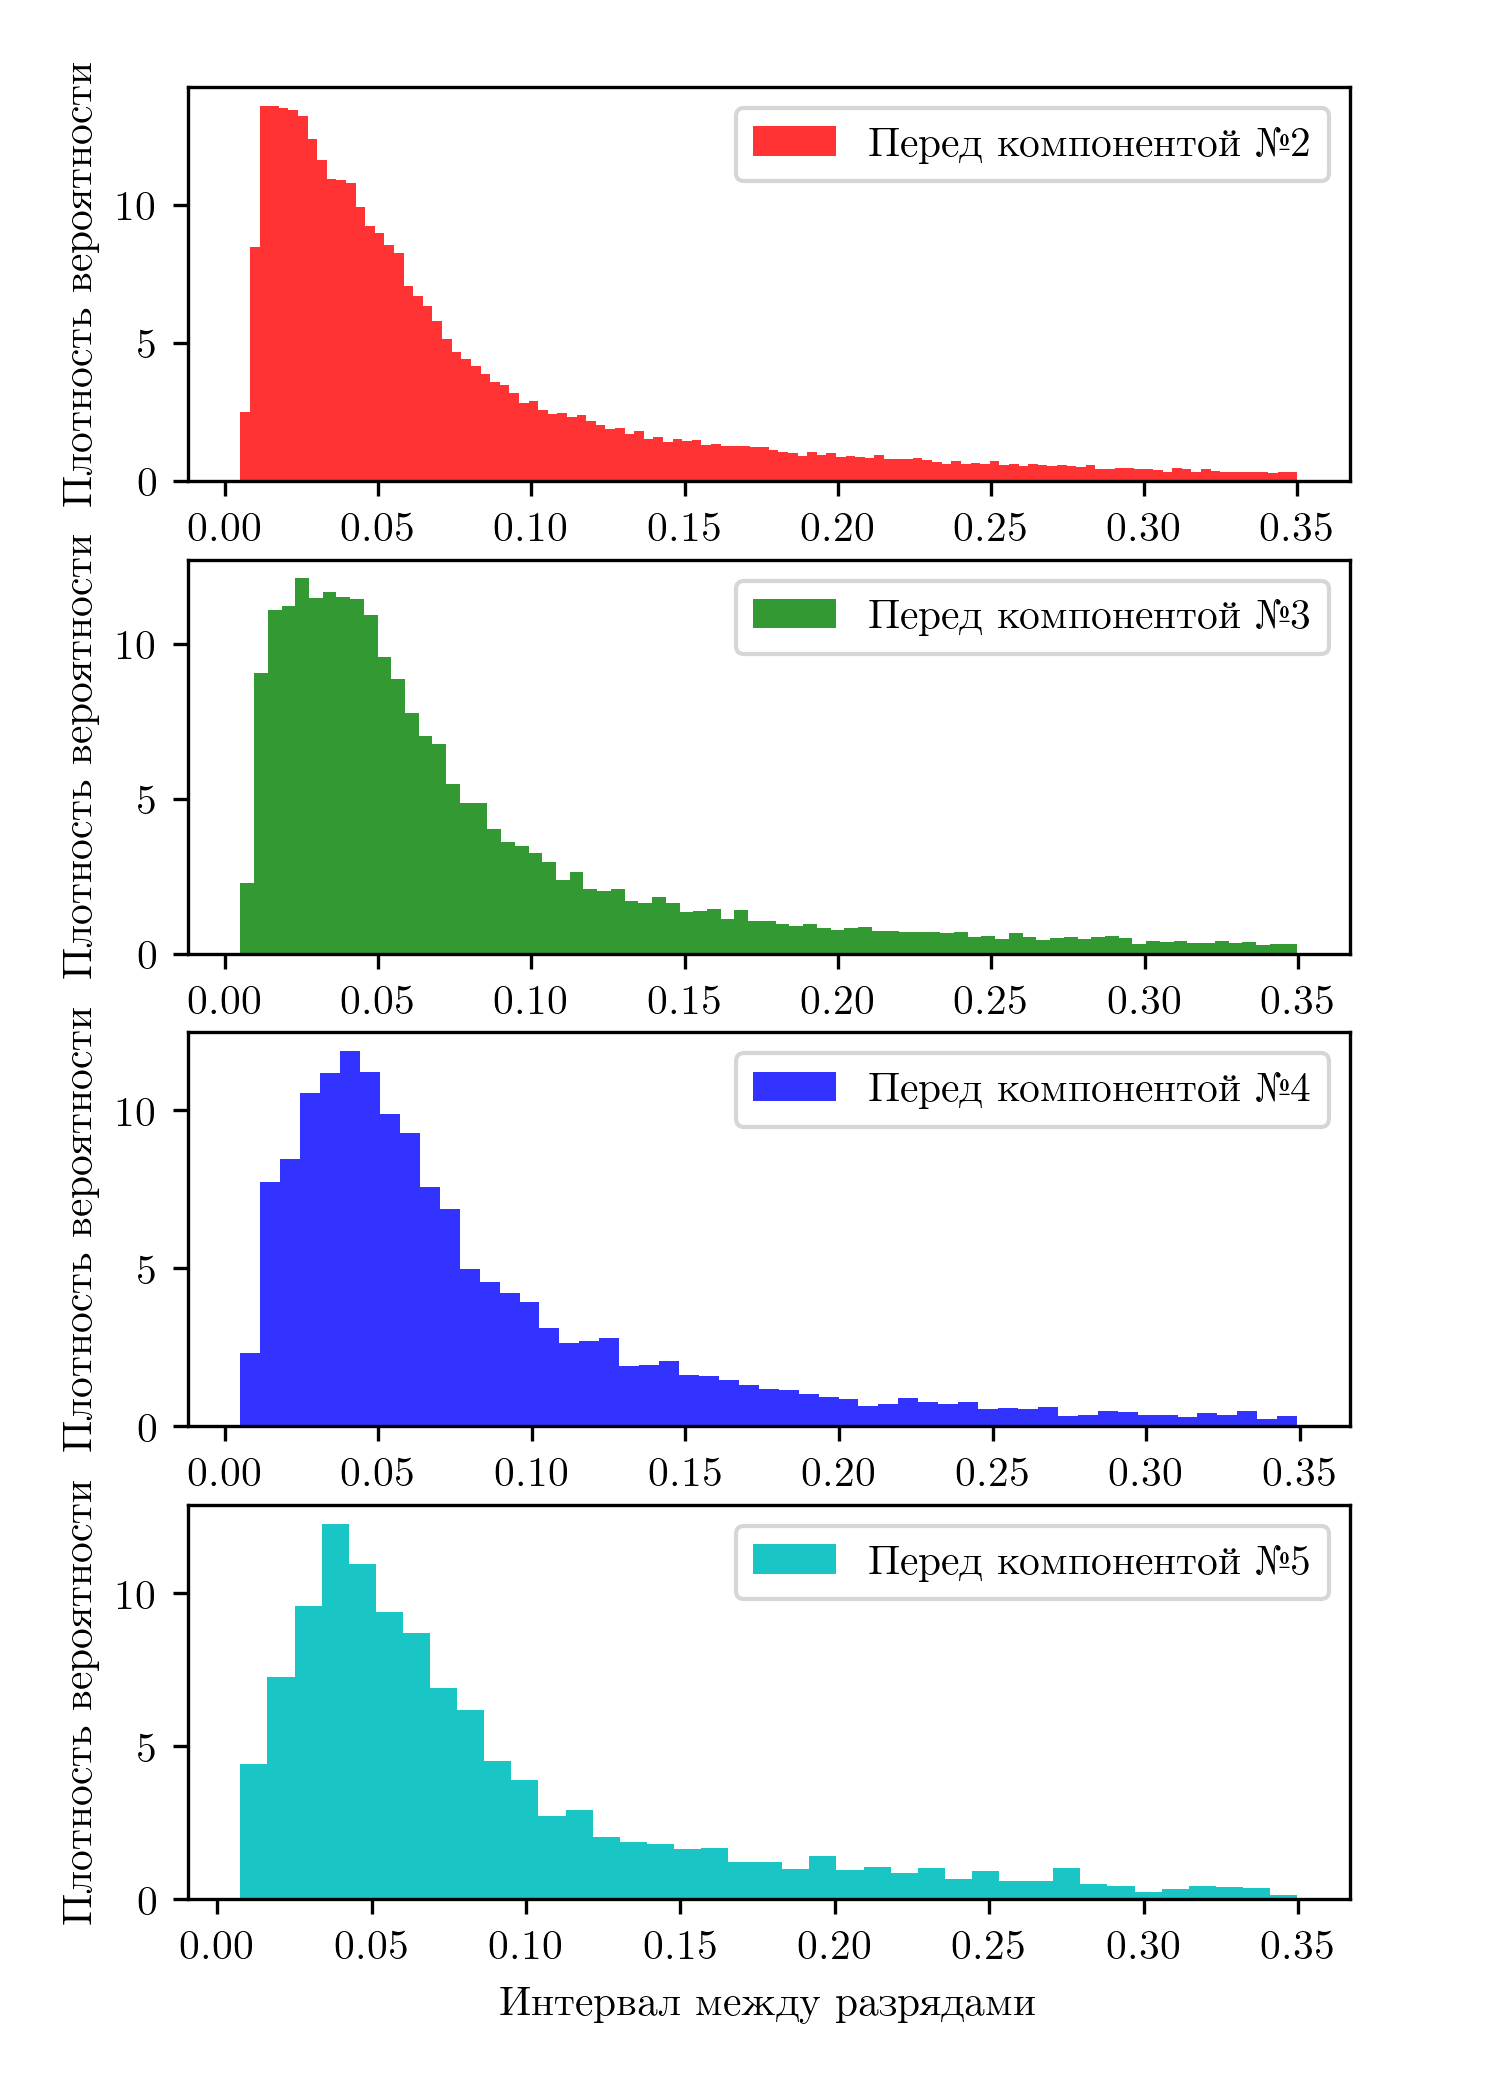
\includegraphics[width=0.8\linewidth]{lds-hist.png}}
	\caption{Распределение временных интервалов перед повторными обратными ударами}
	\label{fig:lds-hist}
\end{figure}

\section{Выводы}
Автором разработана и введена в эксплуатацию региональная грозопеленгационная система OpenLDS. ГПС функционирует с 2014\,г., и по данным на 2017\,г. покрывает территорию диаметром~1500\,км. За время работы системы зарегистрировано более 1,5\,млн. как однокомпонентных, так и многокомпонентных молний.

Проведено исследование точности ГПС OpenLDS на основе сравнения её показаний с данными ДМРЛ и WWLLN. Погрешность позиционирования молний системой OpenLDS оценена сверху величиной 3\,км. Также, оценена погрешность WWLLN на территории Нижегородской области.

На основе данных, полученных ГПС, исследована поражаемость молниями территорий различных типов. Предложена гипотеза отрицательного влияния ТЭЦ на количество гроз в непосредственной близости. 

Исследованы особенности статистики повторных компонент молниевых разрядов. Показано, что условная вероятность каждой следующей компоненты растёт и входит в насыщение с ростом количества компонент. Показано, что средний интервал между повторными компонентами растёт. Предложено объяснение данных закономерностей.



\FloatBarrier
           % Глава 1
\chapter{Численная модель стримерно-лидерной стадии молнии}
\label{sec:model-intro}
Моделирование процесса молнии является сложной задачей, характеризующейся большим диапазоном пространственных и временных масштабов процессов, большим количеством эволюционирующих компонент и сложной геометрией, обладающей фрактальной структурой. В силу этих факторов, применимость аналитических методов к данной задаче ограничена, и наиболее перспективным является численное моделирование.

Актуальные подходы к моделированию молнии можно разделить на несколько категорий:
\begin{enumerate}
	\item \textbf{Плазмохимические модели.} Расчитывается стационарная, либо нестационарная кинетика молниевого канала на различных стадиях. Учитываются десятки и сотни плазмохимических реакций. Модели применимы к широкому спектру разрядов, например "--- к моделированию т.\,н. эльфов и спрайтов \cite{Sentman2008}\cite{Kossiy1994}. Однако такие модели вычислительно сложны, и вследствие этого либо нуль-мерны, либо <<1,5-мерны>> "--- предполагают аксиально-симметричную форму канала разряда. Такой подход не позволяет воспроизводить сложную геометрии молниевого разряда. Строго говоря, плазмохимические модели воспроизводят пробой в воздухе, но ещё не молнию.
	\item \textbf{Электродинамические модели.} Описывается изменение распределения зарядов и токов в молниевом канале. Такие модели исключают влияние электрических процессов на геометрию разряда и чаще всего применяются для описания главной стадии молнии. Для воспроизведения процесса инициации молнии их применимость ограничена. 
	\item \textbf{Дискретные модели, клеточные автоматы.} Воспроизводят динамику молниевого канала на этапе его формирования на дискретной сетке. Ячейки сетки могут находиться в состоянии проводимости и быть частью канала. Каждой ячейке соответствует набор динамических переменных, которые эволюционируют во времени. Дискретные модели воспроизводят сложную геометрию молнии, однако имеют строгие ограничения по масштабу и разветвлённости элементов молнии. В силу того, что данные модели являются высокоуровневыми, они требуют параметризаций процессов, происходящих в ячейках расчётной сетки. Выбор параметризации является сложной задачей. Существующие дискретные модели молнии описывают распространение лидера и не рассматривают процесс его возникновения, \textit{стримерно-лидерный переход.} Примерами дискретных моделей служат работы \cite{Iudin2017}
\end{enumerate}

Одним из наиболее важных и неисследованных этапов развития молнии является процесс её инициации \cite{Dwyer2014}. На данный момент не существует единой точки зрения на то, как достаточно длинный для поддержания собственного развития хорошо проводящий лидерный канал формируется в грозовом облаке, максимальная напряженность электрического поля в котором на порядок ниже поля пробоя воздуха \cite{Marshall1995}. Предпринятые многочисленными исследователями попытки решения данной проблемы вылились в набор конкурирующих гипотез, каждая из которых столкнулась с определенными трудностями.

Первый механизм восходит к работам \cite{Loeb1966, Phelps1974, Griffiths1976}, в которых изучалась возможность инициации стримеров с гидрометеоров. Предполагается, что положительный стример зарождается в области усиленного поля, возникающего при поляризации одиночного гидрометеора во внешнем поле или при сближении пары противоположно заряженных гидрометеоров. При этом считается, что развивающаяся с гидрометеора система положительных стримеров или несколько перекрывающихся стримерных систем, развивающихся с соседних гидрометеоров, выносят положительный заряд в направлении роста и аккумулируют отрицательный заряд в точке старта, что, в конце концов, приводит к появлению пучка отрицательных стримеров, растущих в противоположном направлении \cite{Griffiths1976}. Прогреваясь токами поляризации, биполярная стримерная система формирует внутри себя горячий лидерный канал, способный к самостоятельному поддержанию своего дальнейшего распространения. Недостаток данного механизма состоит в том, что для обеспечения устойчивого развития стримерной системы необходимо наличие либо области с электрическим полем, превосходящим максимально наблюдаемые облачные поля \cite{Griffiths1976}, либо гидрометеора с аномально большим аспектным отношением \cite{Dubinova2015}. В моделях, посвященных инициации положительного стримера с гидрометеора (см., например, \cite{Sadighi2015, Cai2017}), указывается также на необходимость предварительной ионизации, источник которой, как правило, не уточняется.

Вторая гипотеза основана на предложенном Гуревичем \cite{Gurevich1992} механизме пробоя на высокоэнергичных убегающих электронах, для которых эффективная сила трения убывает в интервале от 0.1\,кэВ до 1\,МэВ. В данном энергетическом диапазоне электрон может набирать энергию вплоть до 1\,МэВ, при которой сила трения становится достаточной для компенсации ускоряющего действия электрического поля. При удачном месте возникновения первых затравочных убегающих электронов, появляющихся под действием ионизации нейтралов частицами космических лучей, они могут породить электронную лавину, что, в свою очередь, способно привести к электрическому пробою облачной среды. Предполагается, что пробой на убегающих электронах способен создать плазменное пятно, поляризация на границах которого приводит к существенному усилению поля \cite{Gurevich1999}. Если плазма, поляризуясь, локально приобретает форму стримерной головки, запускается описанный выше стримерный механизм формирования лидера молнии \cite{Gurevich1999}. Несмотря на то, что пробой на убегающих электронах требует полей, примерно равных максимальным измеренным в грозовом облаке значениям, необходимая для реализации данного процесса протяженность области сильного поля достигает километра \cite{Gurevich2001}, что противоречит данным наблюдений.

В своей работе \cite{Dwyer2005} Двайер оспаривает возможность данного сценария, указывая на то, что затравочные электроны, произведенные частицами космического ветра, должны иметь большой поперечный разброс, вследствие чего производимая ими плазма будет сильно разреженной. Вместе с тем, Двайер предлагает позитронную модернизацию механизма пробоя на убегающих электронах, в которой развитие разряда поддерживается петлей положительной обратной связи между позитронными и гамма лучами и может привести к возникновению локальной зоны сильного электрического поля вблизи границы распространения разрядной активности, даже несмотря на отсутствие достаточно сильного крупномасштабного электрического поля, необходимого для механизма, предложенного Гуревичем. Проведенные Двайером вычисления показывают, что за счет данного механизма электрическое поле даже в относительно компактной области может достичь значений, превышающих 1\,МВ/м при давлении на уровне моря и, таким образом, поддержать процесс <<традиционного>> пробоя, приводящего к инициации молнии.

Еще один гибридный механизм, соединяющий идею пробоя на убегающих электронах с инициацией положительных стримерных систем с поверхности гидрометеоров, был предложен Петерсеном \cite{Petersen2008}. В рамках данной модели пробой на убегающих электронах обеспечивает наличие предварительной ионизации, необходимой для инициации положительных стримеров с поляризованных локальным полем гидрометеоров. Возникающий пучок положительных стримеров по мере развития накапливает отрицательный заряд в точке своего основания, локально усиливая поле и создавая условия для возникновения противоположно направленных отрицательных стримеров. Менее многочисленные, но более мощные отрицательные стримеры теперь уже биполярной стримерной системы, прогреваясь, формируют канал пространственного лидера и, участвуя в процессе разделения заряда, усиливают поле на периферии разрядной структуры, провоцируя появление еще одной (вторичной) системы положительных стримеров, развитие которой происходит подобным же образом. Далее вторичная стримерная система поляризуется по аналогии с исходной. В ходе совместного развития положительные стримеры вторичной системы сливаются с отрицательными стримерами первичной, создавая единый канал, прогреваемый токами выравнивания потенциала. В результате многократного повторения данного процесса перекрывающаяся и сливающаяся цепочка биполярных стримерных систем формирует канал лидера молнии.

%Дмитрий Игоревич просил убрать этот абзац из введения
%Ризон \cite{Rison2016}, основываясь на многочисленных натурных измерениях, предполагает, что молниевый разряд может инициироваться так называемым быстрым пробоем на положительных стримеров (fast positive breakdown). Полевые измерения, однако, показывают, что появление молний не всегда сопровождается излучением, характерным для данного типа разряда.

Недавно в работе \cite{Iudin2017} был предложен принципиально новый механизм инициации молнии, основанный на индуцированном шумом кинетическом переходе, происходящем в стохастическом поле заряженных гидрометеоров. Результатом неравновесного фазового перехода являются пятна ионной плазмы с линейными размерами, достигающими нескольких дециметров, и временем жизни порядка нескольких десятков миллисекунд (см. также \cite{todo}). При этом в работе \cite{Iudin2017} подчеркивается, что резкий рост ионной проводимости происходит в экспоненциально редких компактных областях пространства на фоне исчезающе малых изменений средней проводимости среды. В ходе поляризации, обусловленной крупномасштабным электрическим полем грозы, поле на концах плазменных пятен усиливается до величины, достаточной для инициации положительных стримеров. По мере роста концентрации пятен ионной плазмы, коллективная динамика положительных стримерных систем обеспечивает появление лидерного канала в соответствие с качественной картиной описанных выше сценариев Леба и Петерсона, основанных на традиционной доктрине электрического пробоя в атмосфере.

Построение количественной модели зарождения молниевого разряда, основанной на предложенном в работе \cite{Iudin2017} механизме инициации положительных стримеров с поляризованных ионных областей, обладающих повышенной проводимостью, составляет содержание данной главы. Настоящая работа является инновационным развитием модельного подхода \cite{IudinRakov2017}, в котором изложены базовые принципы стохастического развития древа молниевого разряда как саморазвивающегося направленного динамического графа с нелинейными связями. В данной работе решен целый ряд актуальных для моделей развития молниевых разрядов проблем. Во-первых, в предложенной модели впервые отсутствует привязка вершин проводящих связей к узлам пространственной решетки, то есть направление роста разрядного канала не имеет принципиальных ограничений, свойственных всем остальным подобным моделям, в которых морфология разрядных структур ограничена шагом пространственной решетки. Такой подход не ограничивает ни минимальное расстояние между близко расположенными разрядными каналами, ни число связей, растущих из одной вершины. Во-вторых, в настоящей модели впервые последовательно учитывается асимметрия полей развития положительных и отрицательных стримеров. В-третьих, в модели реализован самосогласованный механизм стримерно-лидерного перехода, происходящего посредством развития протекающей в пучке стримерных каналов ионизационно-перегревной неустойчивости. Данные свойства модели позволили успешно воспроизвести основные особенности коллективной динамики множества одновременно развивающихся стримерных разрядов, которая, как это следует из результатов моделирования, является принципиальной основой формирования билидерного канала молниевого лидера в грозовом облаке.

\section{Постановка задачи}
\label{sec:model-base}
В данной работе моделируется развитие молниевого разряда в области однородного крупномасштабного электрического поля грозы с размерами порядка сотен метров. Предполагается, что область пространства, в которой начинает развиваться разрядное дерево, находится на высоте 6~км над уровнем моря, что характерно для исходной точки развития молниевого разряда типа облако-земля \cite{Rison2016}. Напряженность однородного вертикально ориентированного электрического поля $\vec E_{ext}$, в котором формируется разряд, составляет~$2,7 \text{кВ}/\text{см}$, что соответствует максимальному измеренному в грозовом облаке значению \cite{Marshall1995}. В связи со значительной удаленностью разрядного древа от поверхности земли (максимальное расстояние между отдельными узлами разряда много меньше расстояния до земли) в данной модели расчет электрического поля происходит без учёта отраженного в ней заряда. В целях оптимизации расчетов моделирование происходит с автоматическим выбором шага по времени. Характерный временной шаг составляет $10^{-11} - 10^{-9}$~c.

Электрическая цепь, образуемая проводящими структурами молниевого разряда, моделируется в виде динамического графа, вложенного в трехмерное пространство. Базовыми элементами модели являются вершины и рёбра графа. Вершины соответствуют ёмкостным элементам цепи, а рёбра~"--- резистивным. Пример фрагмента такого графа представлен на рис.~\ref{fig:net-frag}. 

В отношении разработанной модели применяется термит <<транспортная самоорганизующаяся модель>> (ТСМ) "--- способ моделирования физических систем, в которых происходит перенос динамических переменных в пространстве в соответствии с геометрией, определяемой этими динамическими переменными.

В процессе инициации молнии возникает сложная система стримеров и развивается лидер. 
Эти объекты образуют разветвлённую электрическую цепь, которую можно представить в виде графа, вложенного в трёхмерное пространство, структура которого меняется с течением времени. Пример фрагмента такого графа представлен на \figRef{fig:net-frag}. Вершинам и рёбрам графа сопоставляются определённые параметры и динамические переменные. По мере совершенствования модели набор динамических переменных и параметров может дополняться и изменяться.

\begin{figure}[h]
	\center{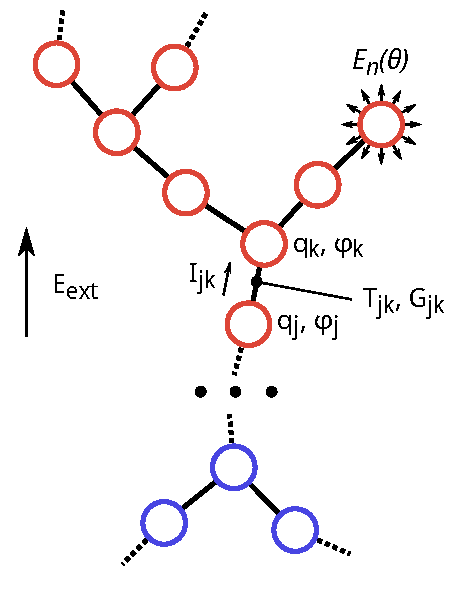
\includegraphics[width=0.5\linewidth]{net-frag.pdf}}
	\caption{Молниевый разряд в виде графа}
	\label{fig:net-frag}
\end{figure}

Каждой вершине графа с индексом $i$ соответствует динамическая переменная $q_i$~"--- сосредоточенный в ней электрический заряд. Каждому ребру с индексом $j$ ставится в соответствие удельная проводимость~$G_j$ и температура нейтрального газа~$T_j$, которые также являются динамическими переменными задачи. Параметром вершины является её эффективный радиус~$R=3\,\text{см}$. Все рёбра представляют собой цилиндры и имеют одинаковые длины~$l=30\,\text{см}$ и радиусы $r=1,4\text{мм}$. Таким образом, с точки зрения электродинамики, система представляет собой совокупность идеально проводящих сфер, соединенных проводниками с конечными проводимостями, благодаря чему модель учитывает распределенную ёмкость проводников. Индуктивности каждой отдельной связи и образуемых ими электрических цепей считаются пренебрежимо малыми.

Эволюция системы определяется двумя процессами: изменением динамических переменных, соответствующих вершинам и рёбрам, а также бифуркациями, изменяющими структуру графа. Первый процесс моделирует перераспределение заряда, нагрев, остывание и изменение проводимости различных частей системы, а второй~"--- пространственное развитие разряда.

\subsection{Эволюция динамических переменных}
Электрическое поле в любой точке пространства с радиус-вектором $\vec r$ находится в электростатическом приближении и вычисляется следующим образом:
\begin{equation}
	\begin{gathered}
		\varphi(\vec{r}) = \kelec \sum_{i=1}^{N} \frac{q_i}{|\vec{r}-\vec{r}_i|} + \varphi_{ext} (\vec{r}) \\
		\vec{E}(\vec{r}) = \kelec \sum_{i=1}^{N} \frac{q_i (\vec{r}-\vec{r}_i)} {|\vec{r}-\vec{r}_i|^3} + \nabla \varphi_{ext}(\vec{r})
	\end{gathered}
	\label{eq:coulomb}
\end{equation}
где $N$ "--- количество вершин графа, $r_i$ и $q_i$ "--- координаты и заряд вершины с индексом~$i$, $\varphi_{ext} (\vec{r})$ "--- потенциал, создаваемый внешним электрическим полем $\vec E_{ext}$. Потенциал вершины~$i$, представляющей собой идеально проводящую сферу радиуса $R$, можно представить как
\begin{equation}
	\begin{gathered}
		\varphi_i = \kelec \sum_{j \ne i} \frac{q_j}{|\vec{r}_k-\vec{r}_j|} + \kelec \frac{q_i}{R} + \varphi_{ext} (\vec{r}).
	\end{gathered}
\end{equation}

Эволюция заряда вершины~$i$ описывается уравнением непрерывности
\begin{equation}
	\dot q_i = \sum_{j=1}^{N_i} I_j,
\end{equation}
где $N_i$ "--- кратность вершины $i$, а $I_j$ "--- ориентированные токи, втекающие в вершину $i$ или вытекающие из нее по примыкающим к данной вершине рёбрам. Ток, текущий по ребру $j$, определяется его проводимостью и разностью потенциалов на его концах:
\begin{equation}
	I_j = G \frac{\pi r^2}{L}(\varphi_{j1} - \varphi_{j2})
\end{equation}
где $r$ и $L$ "--- радиус и длина ребра, $\varphi_{j1}$ и $\varphi_{j2}$ "--- потенциалы соединяемых ребром вершин.

В процессе развития разряда происходит увеличение температуры сосредоточенного в нем нейтрального газа. Когда температура канала превышает характерный порог $T^* = 3000\,K$, развивается ионизационно-перегревная неустойчивость. Эволюцию температуры нейтрального газа в объёма ребра $k$ можно описать как:
\begin{equation}
	\frac{dT_k}{dt} = \frac{1}{\pi L_k R_k^2 \rho c } I_k (\varphi_{k1} - \varphi_{k2})
	\label{eq:temp-evo}
\end{equation}
где $c=1\,\text{кДж}/(\text{кг}\cdot\text{К})$ "--- удельная теплоёмкость воздуха, $\rho=0,63\,\text{кг}/\text{м}^3$ "--- его плотность. Выражение~\eqref{eq:temp-evo} описывает джоулев нагрев газа в приближении отсутствия потери тепла за счёт теплового потока с поверхности канала. Это допустимо, так как процесс теплопередачи в воздухе на масштабах порядка радиуса канала происходит существенно дольше, чем развитие модельного разряда ($1\-2$\,мс).

Эволюция проводимости ребра $k$ и параметризация развития ионизационно-перегревной неустойчивости описывается следующим образом:

\begin{equation}
	G_k = [1-\alpha(T_k)] G_k^I + \alpha(T_k) G_k^{II}
	\label{eq:ioi-param}
\end{equation}
\begin{equation}
	\frac{dG_k^I}{dt} = \left[ \eta \left( \frac{\varphi_{k1} - \varphi_{k2}}{L_k}\right)^2 - \beta \right]G_k^I
	\label{eq:cond-no-ioi}
\end{equation}
где $G_k^I$ и $G_k^{II}$ "--- характерные проводимости канала до и после развития неустойчивости соответственно, $\alpha(T)$ "--- сглаженная степ-функция, описывающая скачкообразный переход от стримерной проводимости к лидерной, происходящий при приближении температуры канала к пороговому значения $T^* = 3000\,K$:
\begin{equation}
	\alpha(T) = \begin{cases}
		0, & T<T^*-50\,K\\
		0,5 + \sin\left[\frac{\pi}{2}\frac{T-T^*}{100}\right], & 2950\,K \le T \le 3050\,K\\
		1, & T<T^*+50\,K\\   
	\end{cases}
	\label{eq:alph-param}
\end{equation}

Выражение \eqref{eq:ioi-param} параметризует процесс ионизационно-перегревной неустойчивости, приводящей к преобразованию стримерного канала в часть канала <<молодого>> лидера молнии с проводимостью $G_k^{II} = 10\,\text{См}/\text{м}$. 
%Величина $G_k^{II}$ принимается константой. - и так понятно, раз написано, чему она равна.
% (максимально допустимая для данной модели проводимость) -- это неудачная формулировка. Есть модель, есть разностная схема, есть точность вычислений вещественных переменных

Уравнение \eqref{eq:cond-no-ioi} описывает эволюцию проводимости до начала развития ионизационно-перегревной неустойчивости. Параметры $\eta = 4.3\cdot10^{-5}\,(\text{В}/\text{м})^{-2}\text{с}^{-1}$ и $\beta = 2,5\cdot10^6\,\text{с}^{-1}$ отвечают за рост температуры канала в результате выделения Джоулева тепла и её  диссипацию соответственно.

Через параметры $\beta$ и $\eta$ можно выразить критическое поле поддержания существования пучка стримеров:
\begin{equation}
	E_{s}^* = \sqrt{\frac{\beta}{\eta}}
\end{equation}
% todo: указать значение этого поля
\subsection{Бифуркации}
\label{sect:bifurcations}
Разработанная модель описывает следующие виды бифуркаций системы, возникающие при определённых условиях:
\begin{enumerate}
	\item Возникновение новой вершины, связанной со старой ребром. Данный процесс моделирует рост и ветвление стримеров.\label{emun:bif-new}
	\item Возникновение ребра между двумя существующими вершинами. Моделирует пробой воздуха между уже имеющимися компонентами разряда.\label{emun:bif-connect}
	\item Исчезновение ребра. Моделирует гашение стримера при исчезновении проводимости.\label{emun:bif-remove}
\end{enumerate}
Далее рассмотрим детально каждый из этих процессов. 

\highlight{Бифуркация типа \ref{emun:bif-new}.} Рост моделируемого разряда происходит посредством возникновения новых вершин графа, соединенных новыми рёбрами с уже существующими вершинами. Каждые новообразованные вершина и ребро ассоциируется с однонаправленным пучком стримеров одинаковой полярности длиной $L_0 = 30\,\text{см}$. Задача моделирования каждого стримера по отдельности имеет слишком большую вычислительную сложность и нереализуема в рамках используемого подхода.

Для параметризации процесса ветвления разряда рассмотрим небольшой плоский элемент поверхности некоторого электрода площадью $\Delta S$ (\figRef{fig:electode}). Пусть вблизи поверхности электрода имеется электрическое поле~$\vec E$. 
\begin{figure}[h]
	\center{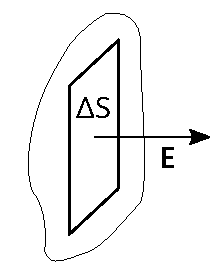
\includegraphics{electrode.pdf}}
	\caption{Элемент поверхности произвольного электрода}
	\label{fig:electode}
\end{figure}

Вероятность возникновения стримера с элемента площади $\Delta S$ за малое время $\Delta t$ можно записать, как
\begin{equation}
	P_s(E_n, \Delta S, \Delta t) = f(E_n)\Delta S \Delta t
	\label{eq:prob-deltas}
\end{equation}
где $E_n$ "--- нормальная компонента электрического поля, $f(E_n)$ "--- зависящая от поля вероятность возникновения стримера в единицу времени на единицу площади поверхности проводника. Функция $f(E_n)$ определяется составом газовой среды. Для стримерного разряда в воздухе функция $f(E_n)$ зависит от направления электрического поля на поверхности электрода. Таким образом, модель учитывает асимметрию критических полей развития стримеров положительной и отрицательной полярностей, причем отрицательные стримеры, в соответствии с многочисленным экспериментам \cite{Bazelyan1997}, имеют вдвое большие критические поля. Заметим, что $f(E_n)$ не является плотностью веротяности и поэтому не нормирована на единицу. Её физический смысл "--- количество возникающих стримерных разрядов на~$1\,\text{м}^2$ за 1~с при заданном поле $E_n$.

Выражение~\eqref{eq:prob-deltas} может быть записано в виде дифференциалов:
\begin{equation}
	dp_s(E_n) = f(E_n)dS dt
	\label{eq:prob-diff}
\end{equation}

В рамках рассматриваемой модели роль электродов, дающих начало пучкам стримеров, то есть новым ребрам и вершинам графа, играют идеально проводящие сферы, расположенные в вершинах графа. Распределение электрического поля на поверхности сферы во внешнем поле $\vec E_0$ описывается следующим выражением:
\begin{equation}
	E_n(\theta) = 3|\vec E_0 | \cos \theta + E_1 ,
	\label{eq:e-on-sphere}
\end{equation}
где $\vec E_0$ "--- внешнее по отношению к рассматриваемой сфере поле, создаваемое постоянным вертикальным полем $E_{ext}$ и зарядами, сосредоточенными на всех прочих вершинах графа, $\theta$ "--- угловая координата точки на сфере относительно направления внешнего поля $\vec E_0$, $E_1$ "--- собственное поле сферы, которое при величине ее заряда $q_i$ и радиусе $R$ может быть найдено как
\begin{equation}
	E_1 = \kelec \frac{q_i}{R}.
\end{equation}

Используя \eqref{eq:prob-diff} и \eqref{eq:e-on-sphere} для любого малого промежутка времени $dt$ можно сгенерировать случайное событие <<возникновение стримера>> методом Монте-Карло. Более подробно принцип генерации этого события рассмотрен в разделе \ref{sec:streamer-generation}. В качестве расстояния, на которое новая вершина удалена от уже имеющейся, принимается константа $L_0$, одинаковая для всей модели. Величина $L_0$ выбирается достаточно маленькой, чтобы между ветвлениями стримера успевало возникнуть несколько не ветвящихся участков.

Отметим, что узлы динамического графа могут располагаться сколь угодно близко друг к другу. Направление ветвления моделируемых проводников определяется методом Монте-Карло из полного диапазона телесных углов, равного $4\pi$ стерадиан. Степень ветвления вершины ограничивается лишь локальным значением электрического поля, то есть один и то же узел, в принципе, может быть источником для неограниченного числа рёбер. Для сравнения, в случае моделей, использующих пространственную решетку, число соседних узлов и, следовательно, возникающих из одной вершины связей, всегда конечно и ограничено числом 26. Таким образом, в данной модели структура проводников и их связность может быть гораздо более богатой, чем в случае моделей, использующих пространственные решетки.

\highlight{Бифуркация типа \ref{emun:bif-connect}.} Параметризация процесса образования новой связи между уже имеющимися узлами $i$ и $j$ системы происходит при выполнении следующих условий:
\begin{enumerate}
	\item Величина среднего поля между вершинами больше пороговой:
	\begin{equation}
		\frac{|\varphi_i - \varphi_j|}{L_{i,j}} > E^*
		\label{eq:conn-condition-1}
	\end{equation}
	где $L_{i,j}$ "--- расстояние между вершинами, $E^*$ "--- пороговое поле
	\item Вершины расположены достаточно близко:
	\begin{equation}
		L_{i,j} > \xi L_0
		\label{eq:conn-condition-2}
	\end{equation}
	где $\xi$ "--- коэффициент порядка $1\ldots10$.
\end{enumerate}
В расчётах величина порогового поля $E^*$ принимается равной $3\cdot10^5\,\text{В}/\text{м}$, коэффициент $\xi = 3$.

\highlight{Бифуркация типа \ref{emun:bif-remove}.} Отмирание ребра графа $k$ происходит при падении его проводимости, определяемой \eqref{eq:ioi-param}, ниже критического значения. Условие удаления ребра выглядит следующим образом:
\begin{equation}
	G_k < \lambda G_0
\end{equation}
где~$G_0$ "--- начальная проводимость ребра, а~$\lambda$ "--- коэффициент принимаемый в расчётах равным 0,95. Из 	\eqref{eq:temp-evo} и \eqref{eq:ioi-param} следует, что ребро, в котором развилась ионизационно-перегревная неустойчивость, не может исчезнуть.

При отмирании проводящего ребра графа одна или несколько вершин могут оказаться отсоединены от основного канала разряда. Впоследствии они могут снова оказаться <<подключенными>> к разрядной структуре при выполнении \eqref{eq:conn-condition-1} и \eqref{eq:conn-condition-2}, либо же оставаться изолированными, внося вклад в пространственный заряд. Диссипация заряда за время моделирования (порядка 1-2\,мс) считается пренебрежимо малой. За счёт наличия изолированных вершин, окружающих разрядный канал, модель воспроизводит чехол лидера.

\subsection{Генерация события возникновения узлов модельного графа}
\label{sec:streamer-generation}
Рассмотрим более подробно вопрос генерации случайного события возникновения нового пучка стримеров. Процесс пробоя воздуха параметризуется некоторой функцией $f(E)$ согласно формуле \eqref{eq:prob-diff}. При этом, согласно \eqref{eq:e-on-sphere}, электрическое поле на поверхности сферы можно записать, как 
\begin{equation}
	E_n(\theta) = 3E_0 \cos \theta + E_1,
\end{equation}
где $E_0$ "--- внешнее поле, вдоль положительного направления которого направлена ось $\theta = 0$, а $E_1$ "--- собственное поле вершины сферической вершины графа. Запишем \eqref{eq:prob-diff} с учётом симметрии:
\begin{equation}
	dp(\theta) = 2\pi R^2 f(E(\theta)) \sin \theta d\theta
\end{equation}
произведя замену переменных $\xi = \cos \theta$, получим дифференциальное распределение
\begin{equation}
	dp(\xi) = -2\pi R^2 f(3E_0 \xi + E_1) dt,
\end{equation}
откуда можно получить интегральную вероятность
\begin{equation}
	dP(\theta<\theta_0) = \frac{2\pi R^2}{3E_0} \left( F(3E_0 + E_1) - F(3E_0 \cos \theta_0 + E_1)\right)dt,
	\label{eq:total-prob}
\end{equation}
где $F(x)$ "--- неопределённый интеграл функции $f$. В обозначении $dP$ присутствует дифференциал, поскольку вероятность по-прежнему записывается для дифференциально малого промежутка времени $dt$.

Для того, чтобы при конкретном $dt$ сгенерировать случайное событие, вероятность которого определяется выражением \eqref{eq:total-prob}, необходимо сгенерировать случайную величину $\zeta$ из интервала $[0, 1)$. Максимальное значение $dP$ достигается при $\theta = \pi$:
\begin{equation}
	dP_{max}(\theta<\theta_0) = \frac{2\pi R^2}{3E_0} \left( F(3E_0 + E_1) - F(-3E_0 + E_1)\right)dt,
	\label{eq:total-prob-max}
\end{equation}
В случае, если $\zeta > dP_{max}$, за выбранный интервал времени $dt$ событие не происходит. В противоположном случае, новый сегмент стримера возникает, и его направление $\theta$ определяется корнем уравнения
\begin{equation}
	F(3E_0 \cos \theta + E_1) =  F(3E_0 + E_1) - \zeta \frac{3E_0}{2\pi R^2 dt},
	\label{eq:theta-equation}
\end{equation}

В силу симметрии задачи, при возникновения нового сегмента стримера, его угловое направление $\varphi$ генерируется из равномерного распределения по интервалу $[0, 2\pi)$.

Разработанный подход к генерации события применим для произвольной функции $f(E)$ при условии численного решения уравнения \eqref{eq:theta-equation}. Поскольку $F = \int f dE$ "--- монотонна, применимы стандартные методы решения алгебраического уравнения, например "--- серединное деление. Для оптимизации расчётов, функцию $F$ нужно однократно табулировать.

Использованные в расчётах парметры приведены в таблице~\ref{tab:parameters}.
\begin{table}[h]
	\caption{Расчётные параметры модели}
	\label{tab:parameters}
	\begin{center}
		\begin{tabular}{l|l}
			Параметр & Значение \\
			\hline
			Внешнее электрическое поле, $E_{ext}$ & $2,7\cdot 10^{5}\,\text{В}/\text{м}$ \\
			Радиус вершины, $R$ & 3\,см \\
			Радиус ребра, $r$ & 1,4\,мм \\
			Длина ребра, $l$ & 30\,см \\
			Плотность воздуха, $\rho$ & $0,63\,\text{кг}/\text{м}^3$ \\
			Удельная теплоемкость воздуха, $c$ & $10^3\,\text{Дж}/(\text{кг}\cdot\text{К})$ \\
			Начальная проводимость ребра, $G_0$ & $1\cdot10^{-10}\,\text{См}/\text{м}$ \\
			Постоянная роста проводимости, $\eta$ & $4.3\cdot10^{-5}\,(\text{В}/\text{м})^{-2}\text{с}^{-1}$ \\
			Постоянная релаксации проводимости, $\beta$ & $2,5\cdot10^6\,\text{с}^{-1}$ \\
			Пороговая температура перегревной неустойчивости, $T^*$ & $3000\,\text{К}$ \\
			%Порог гашения тока, $\lambda$ & 0,95 \\
			Пороговое поле инициации положительных стримеров, $E^+$ & $0.5\cdot 10^{6}\,\text{В}/\text{м}$\\
			Пороговое поле инициации отрицательных стримеров, $E^-$ & $1.0\cdot 10^{6}\,\text{В}/\text{м}$\\
		\end{tabular}
	\end{center}
\end{table}

\section{Результаты моделирования}
\label{sec:model-results}
В данной главе представленная транспортная самоорганизующаяся модель развития искрового разряда в воздухе была применена к изучению процесса инициации лидера молнии.
\begin{figure}[h]
	\center{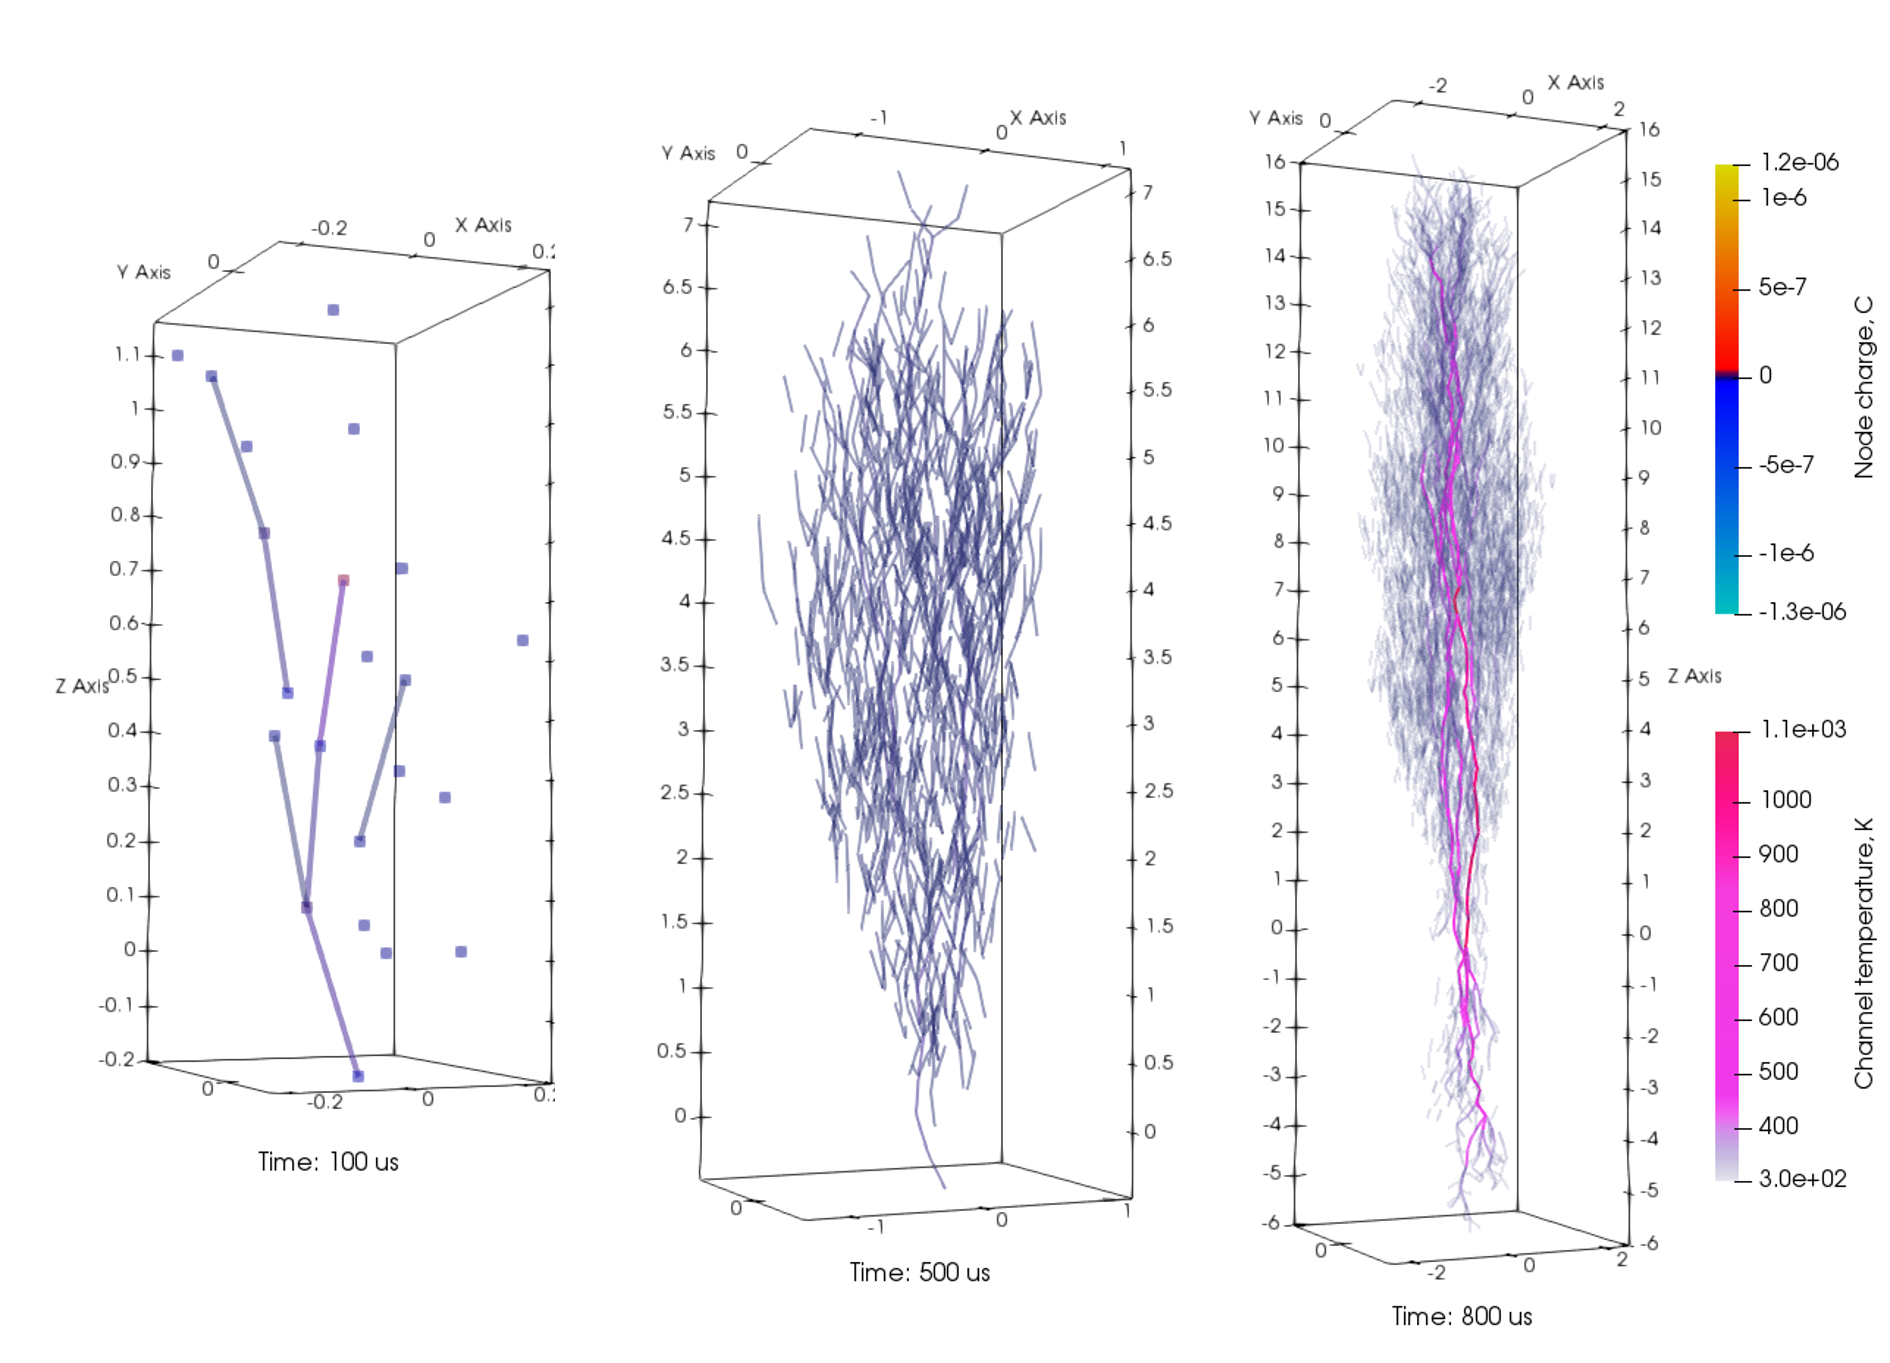
\includegraphics[width=0.8\linewidth]{model-pre-leader.png}}
	\caption{Визуализация долидерной стадии развития модельного разряда. Возникновение первых одиночных стимеров, их объединение в связную токовую структуру и появление первых отрицательных стримеров.}
	\label{fig:pre-leader}
\end{figure}

\begin{figure}[h]
	\center{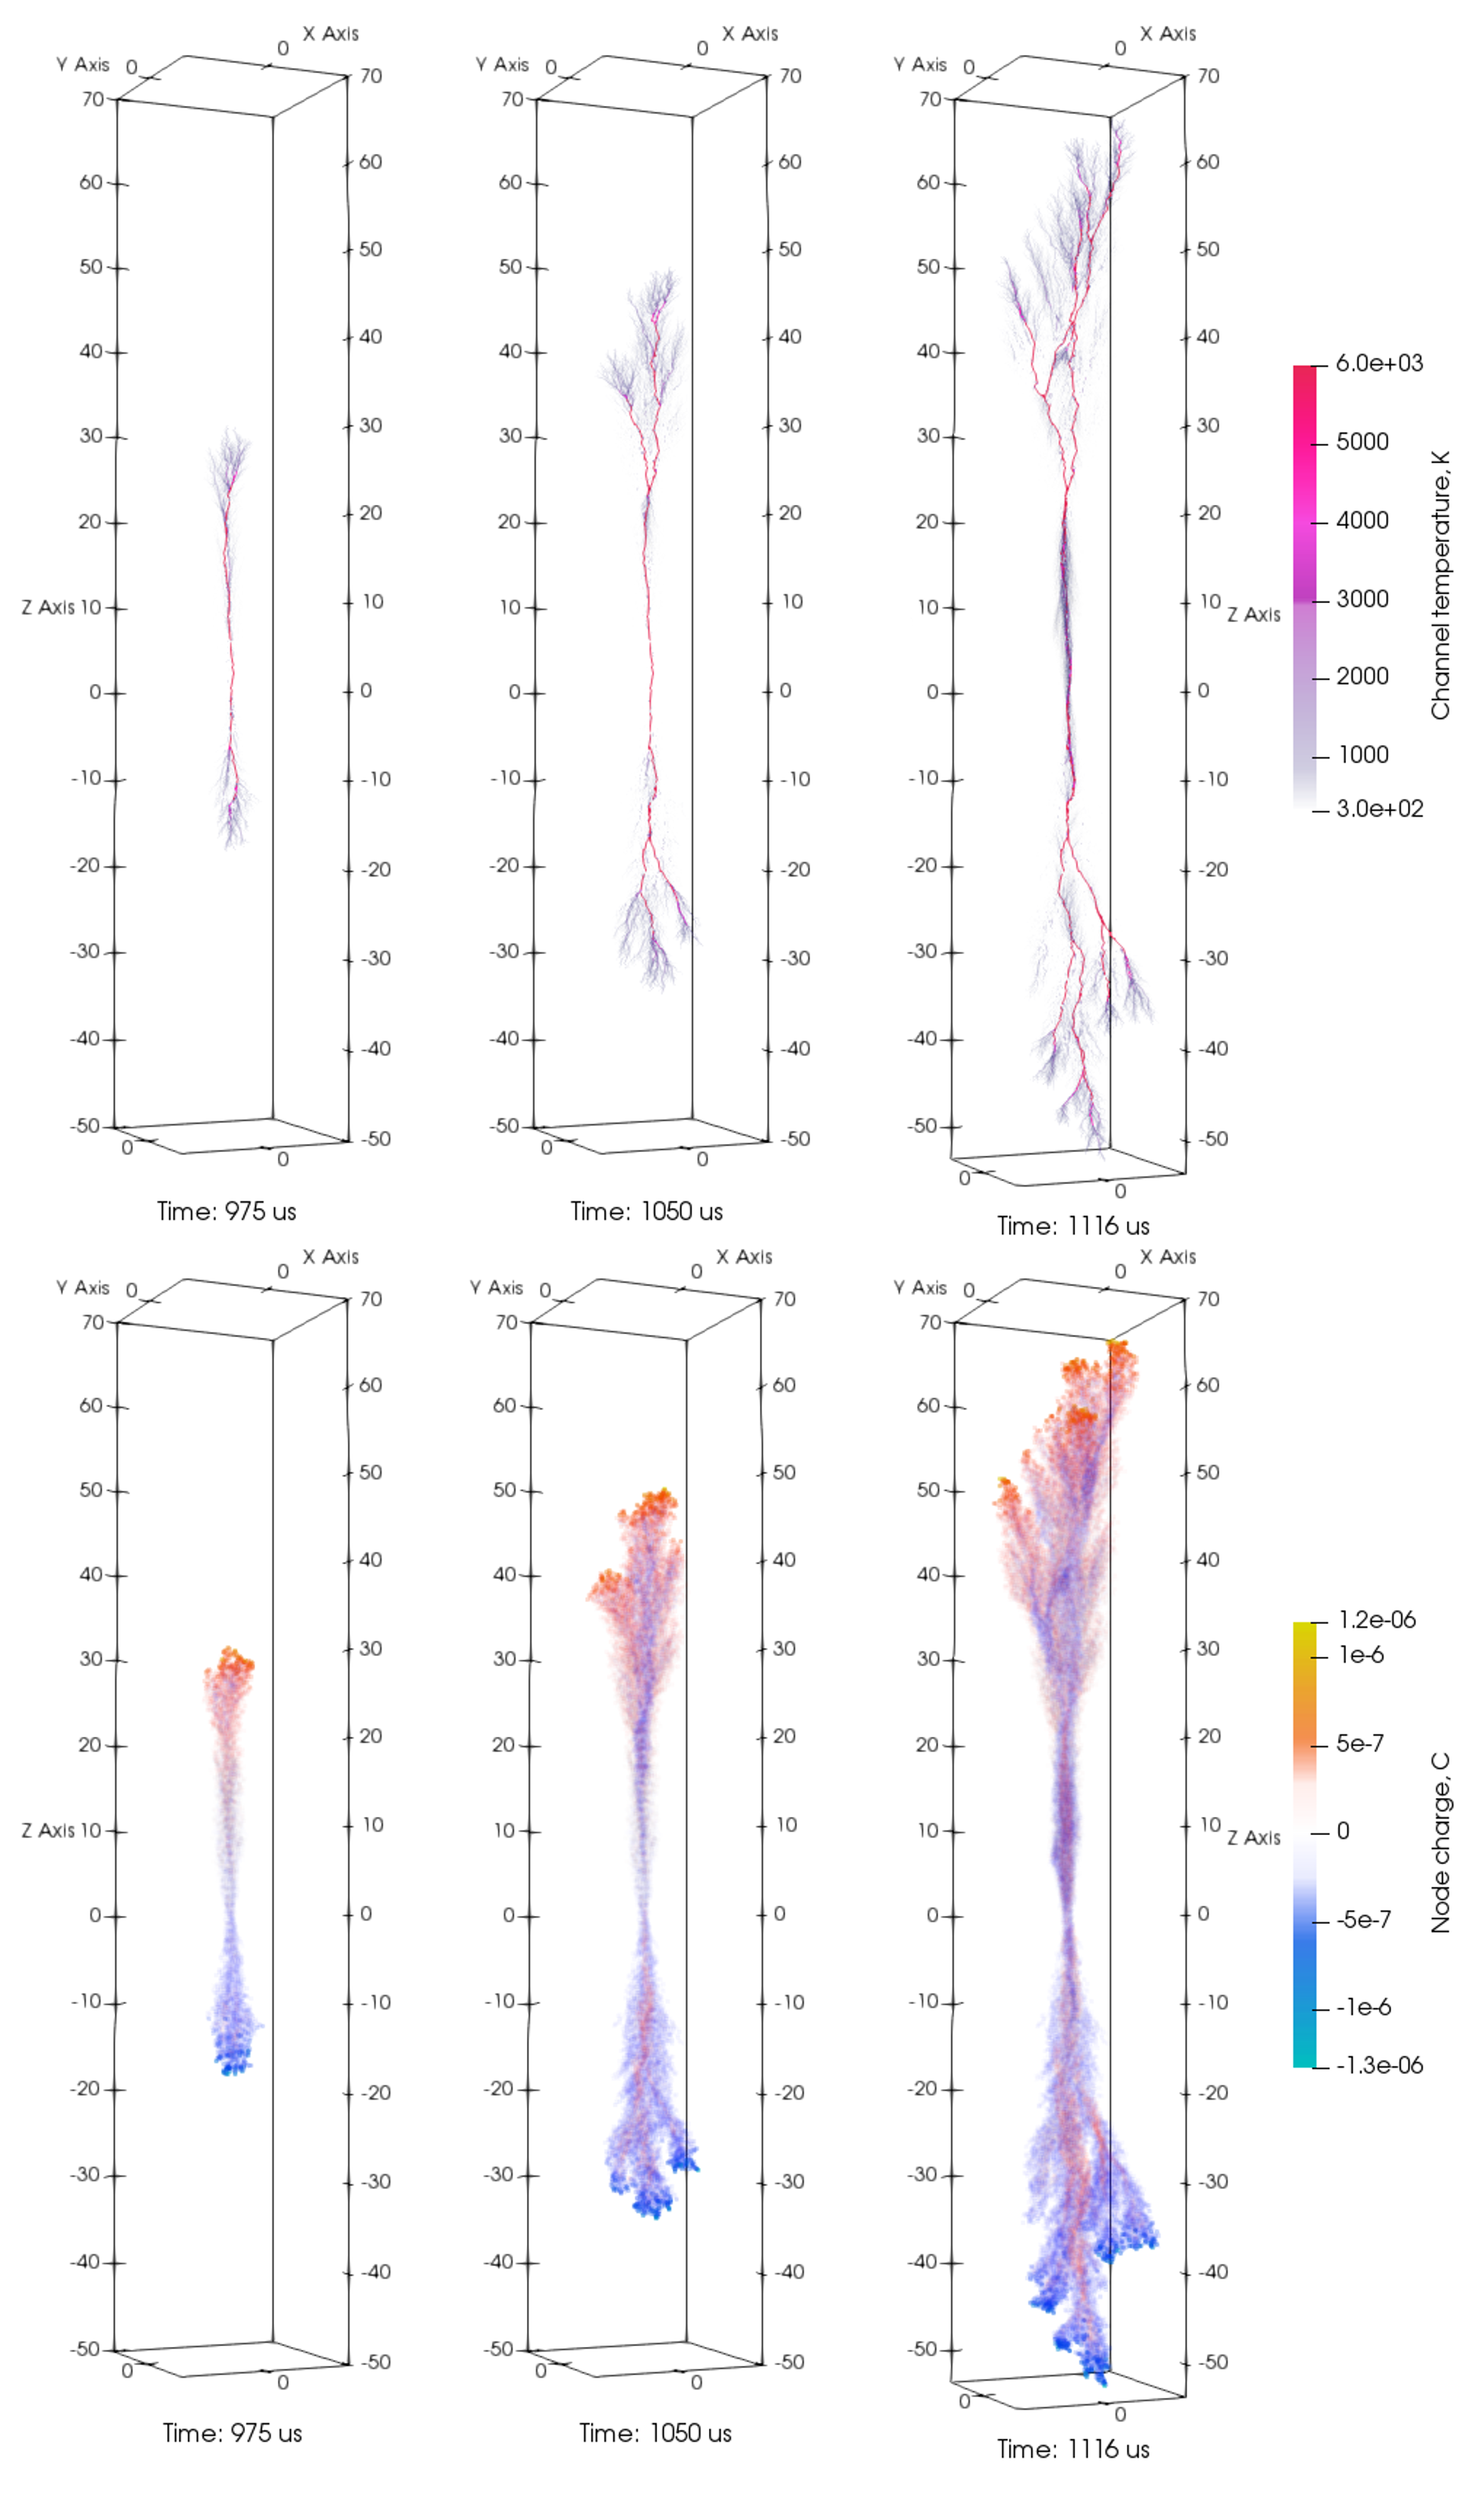
\includegraphics[width=0.8\linewidth]{model-leader-composition.png}}
	\caption{Визуализация лидерной стадии развития молниевого разряда. Распространение биполярного лидера молнии.}
	\label{fig:model-leader-composition}
\end{figure}
На \figRef{fig:pre-leader} показана временная динамика моделирования долидерной части процесса зарождения молниевого канала в облаке. Спустя~$t=100$\,мкс от начала моделирования система состоит всего из 22-х вершин с небольшим количеством перманентно возникающих и гаснущих связей. Электрическое поле, создаваемое разделёнными зарядами, на данном этапе недостаточно для возникновения большего числа стримерных каналов. Через~500\,мкс от начала моделирования количество узлов составляет~3330. Разряд на данном этапе представляет собой совокупность слабо связанных проводников, образующих группы по 2-3~ребра, причем большинство связей гаснет через 10-20\,мкс после появления. Затем число рёбер начинает ускоренно расти, и в момент времени $t = 800$\,мкс наблюдаются устойчивые цепочки связанных проводников, эффективно прогреваемых токами поляризации. При этом общее число узлов модели составляет~25\,тысяч. Электрическое поле на нижнем конце разряда становится достаточным для возникновения отрицательных стримеров.

На \figRef{fig:model-leader-composition} приведена временная динамика моделируемого молниевого канала после возникновения стримерно-лидерного перехода. В верхней части рисунка показаны проводящие структуры, в нижней "--- распределение заряда в пространстве. Начиная с момента времени $t = 927$\,мкс биполярный лидер стремительно развивается двунаправленным образом: его положительная часть распространяется вверх, а отрицательная "--- вниз, причем головки обоих лидеров продвигаются с примерно одинаковой скоростью порядка 210 км/с. К моменту времени $t = 1116$\,мкс число вершин модельного графа возрастает до 484\,тысяч.

На \figRef{fig:model-leader-positive-end} показаны структура проводников и распределение заряда на конце положительной части биполярного лидера молнии в момент времени $t = 1116$\,мкс. Для простоты восприятия на данном рисунке отсутствуют холодные стримерные каналы и узлы, имеющие близкий к нулю заряд.

\begin{figure}[h]
	\center{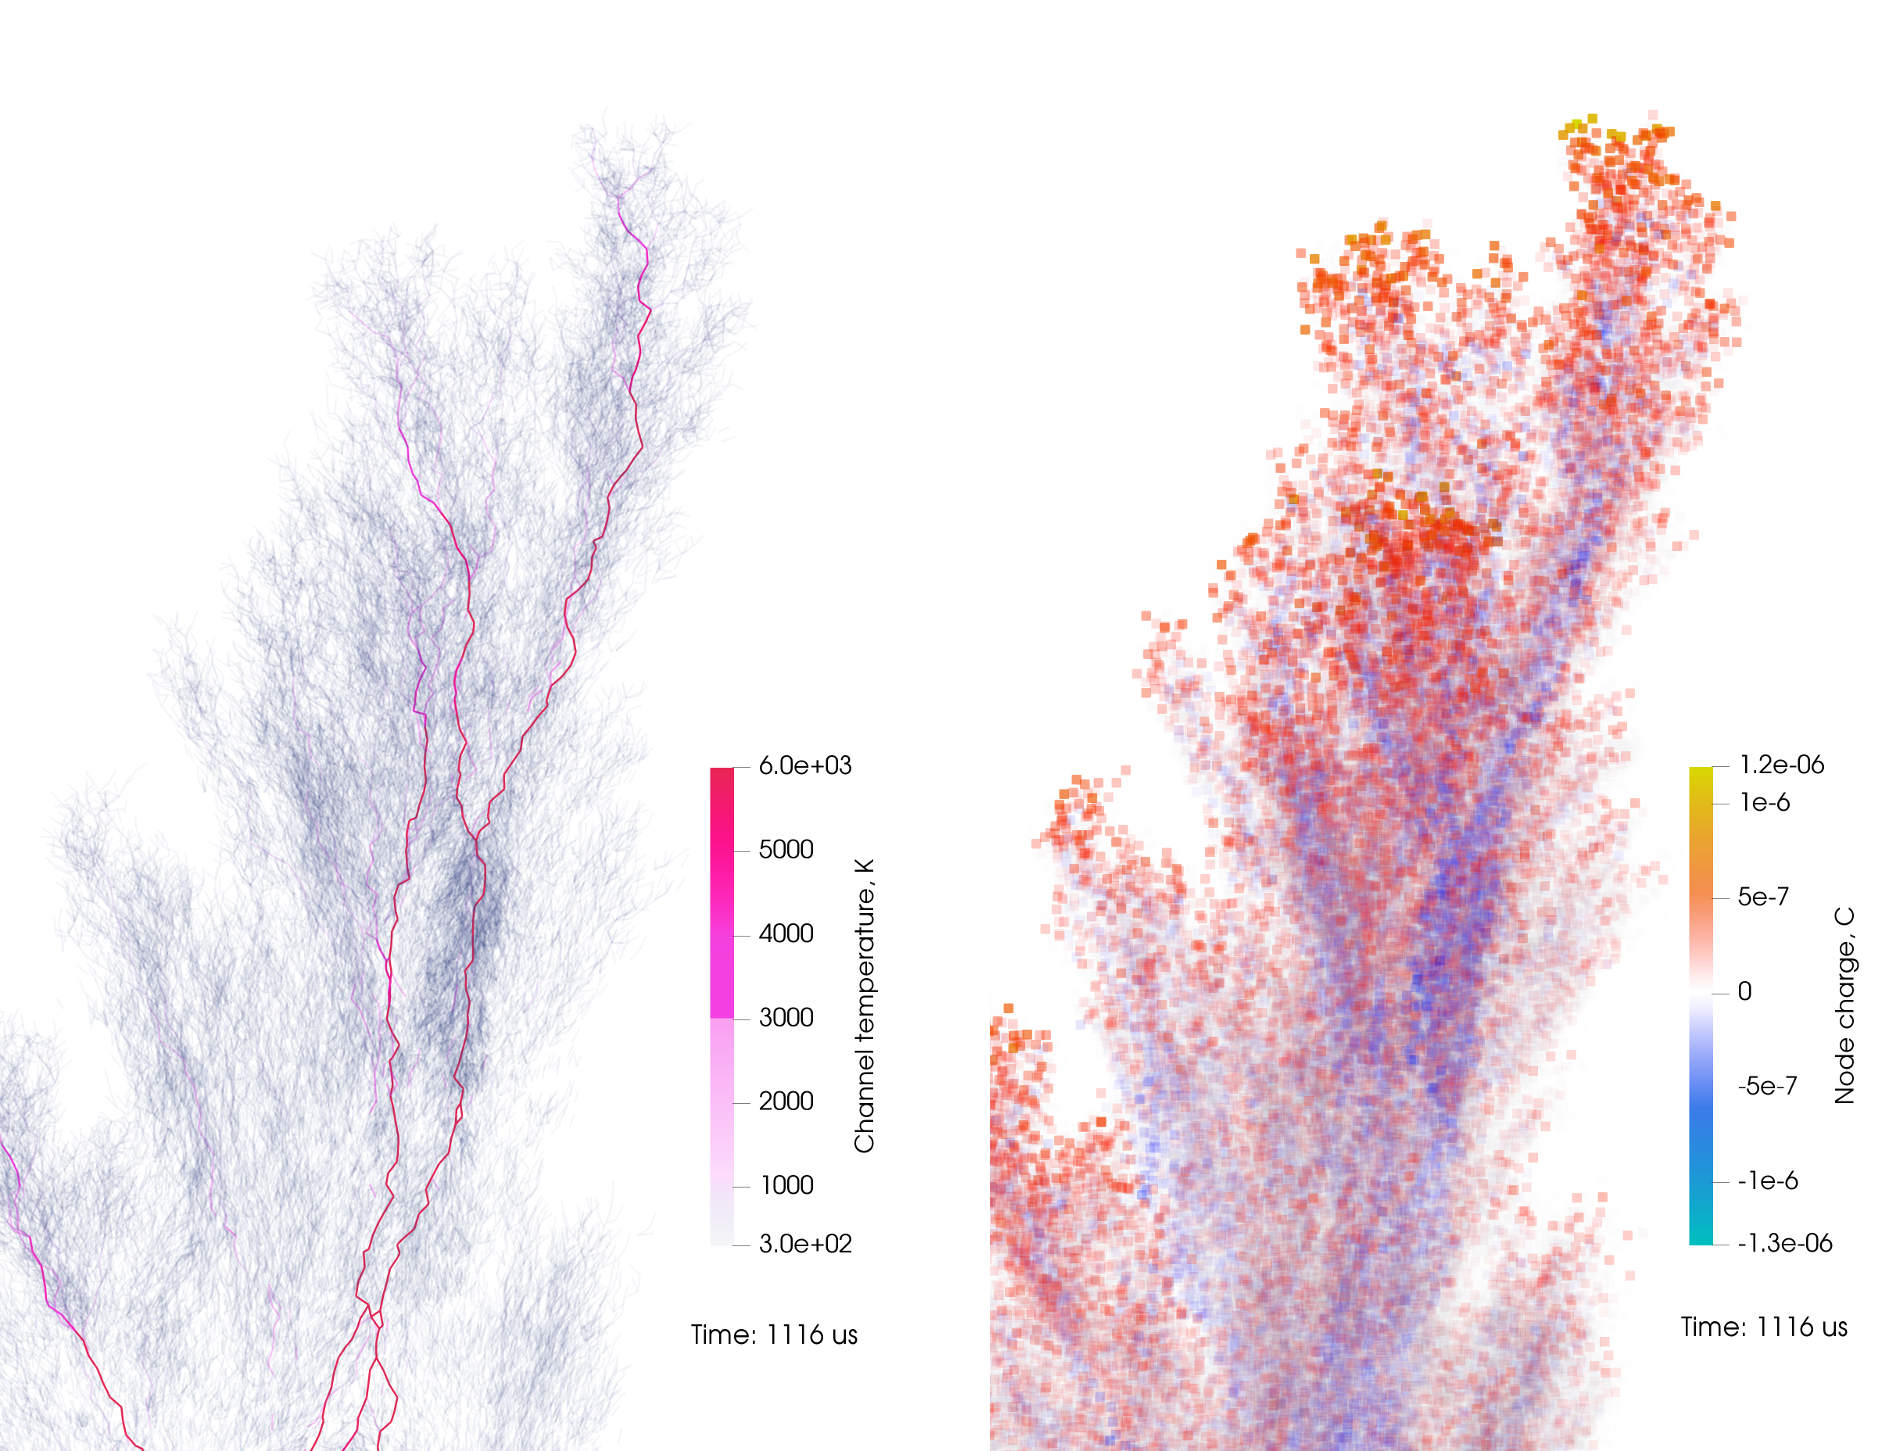
\includegraphics[width=0.8\linewidth]{midel-positive-end.png}}
	\caption{Увеличенный фрагмент  конца положительной часи лидерного канала, визуализирующий структуру проводящих связей и распределение пространственного заряда в момент времени $t = 1116$\,мкс от начала моделирования.}
	\label{fig:model-leader-positive-end}
\end{figure}

\begin{figure}[h]
	\center{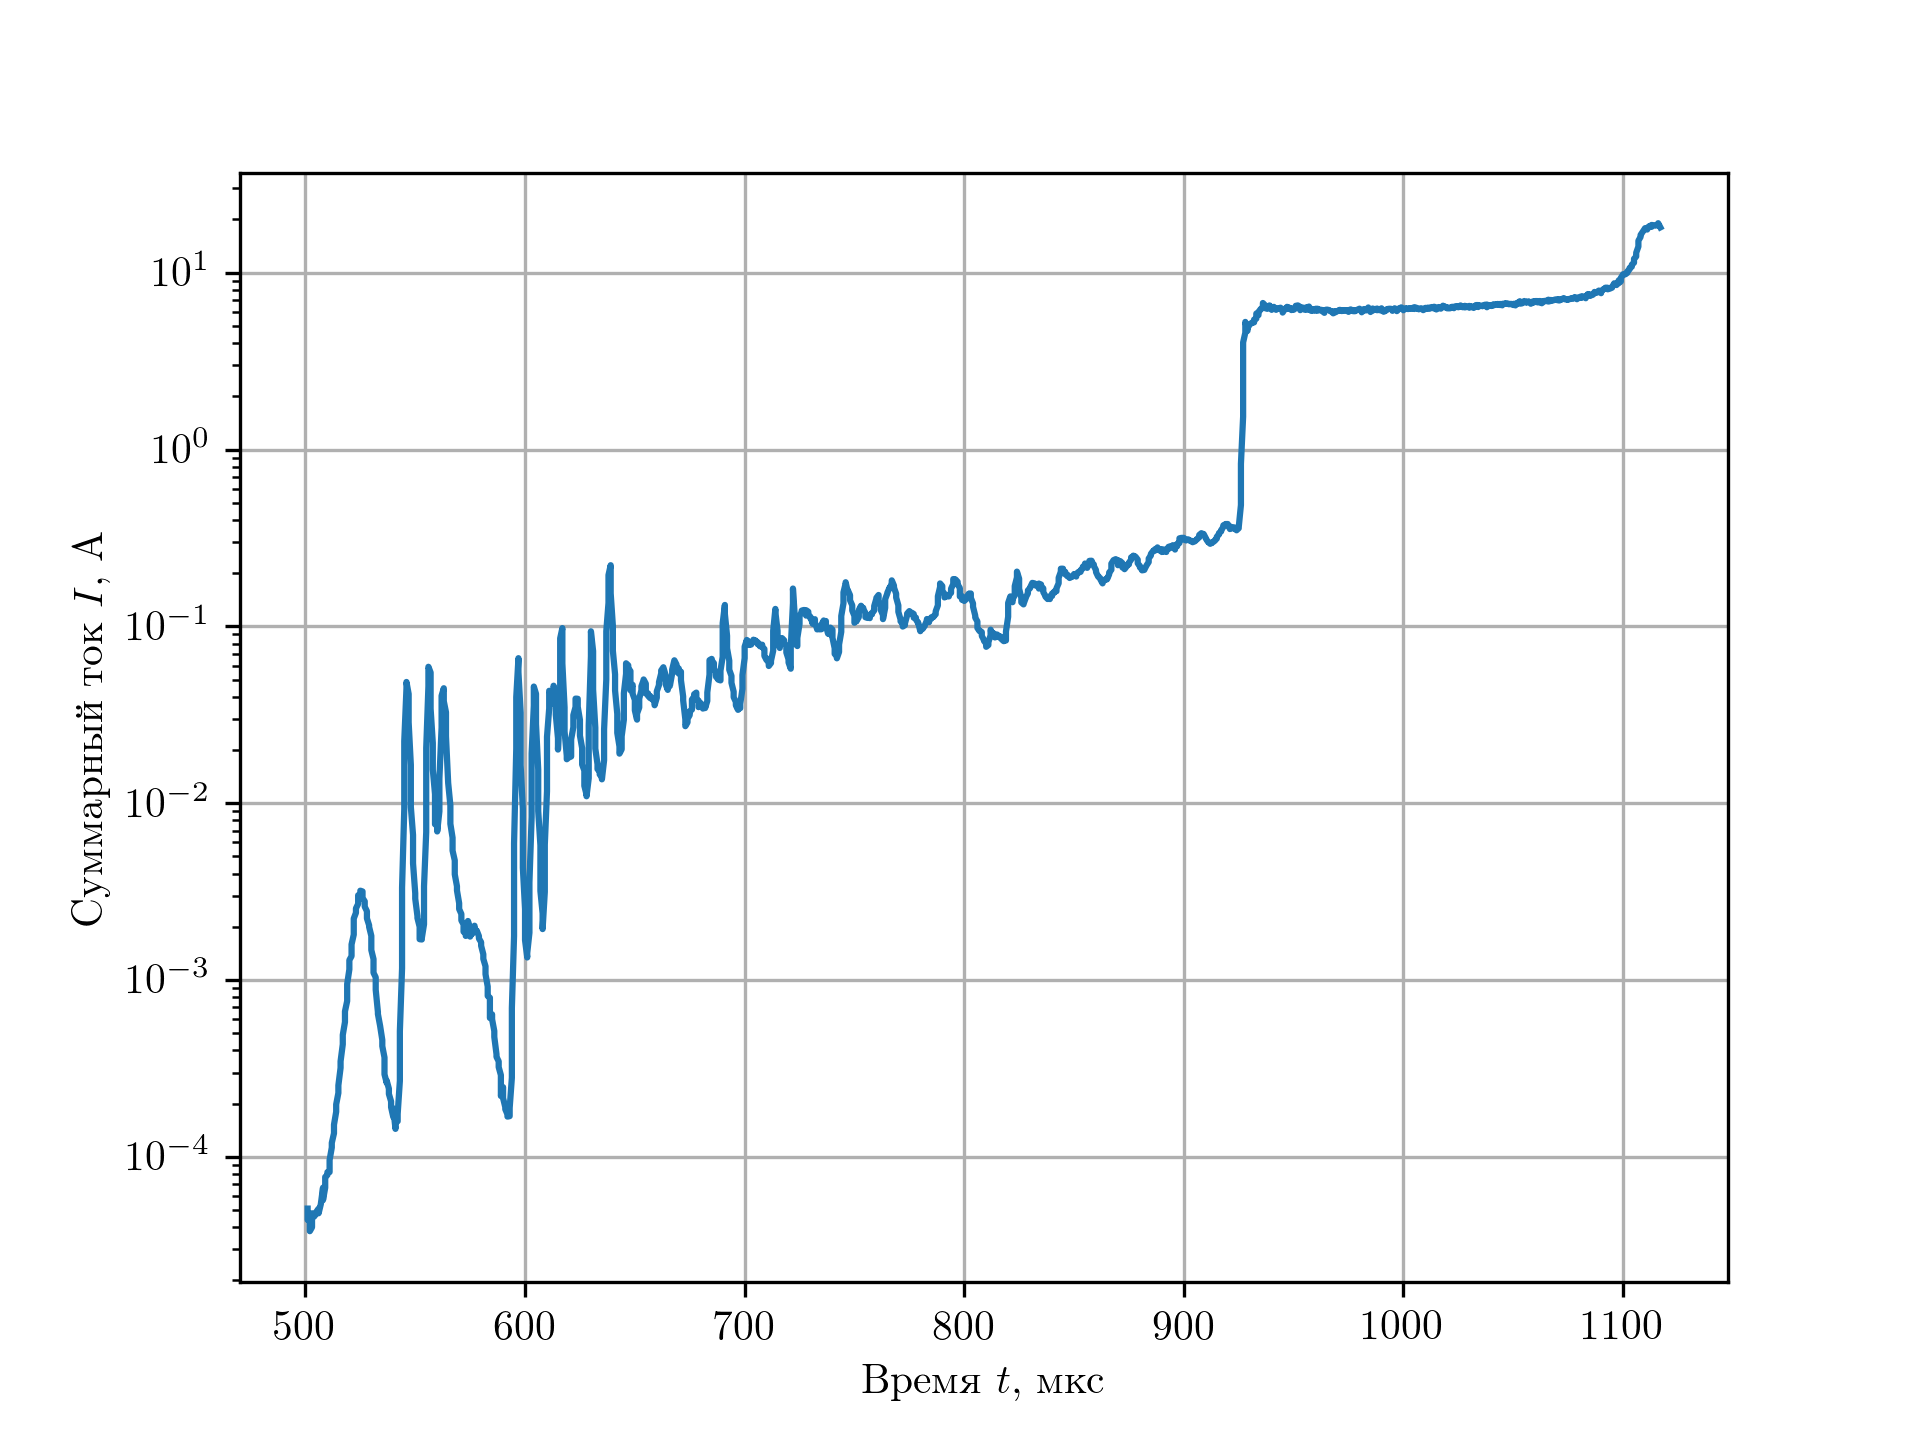
\includegraphics[width=0.8\linewidth]{currents.png}}
	\caption{Осциллограмма тока в канале зарождающегося лидера молнии.}
	\label{fig:full-current-vs-time}
\end{figure}

На \figRef{fig:full-current-vs-time} приведена осциллограмма тока в канале зарождающегося лидера молнии. График приведён с момента времени $t = 500$\,мкс, поскольку до этого отдельные пучки стримеров не образуют связанную цепочку. Начиная с $t = 500$\,мкс, по мере развития коллективного канала ток стабилизируется и постепенно растёт. Увеличение тока на порядок в момент времени $t = 927$\,мкс соответствует сримерно-лидерному переходу "--- возникновению молниевого лидера. Второй, более плавный скачёк тока при $t = 1100$\,мкс соответствует моменту соединения двух ветвей положительной части лидера с образованием петли, что привело к снижению общего сопротивления канала.

\section{Обсуждение результатов моделирования}
\label{sec:model-talks}
Разряд начинает развиваться из простейшей проводящей структуры, образованной парой изначально незаряженных вершин и ребром между ними, поляризация которой происходит под действием внешнего электрического поля. Основываясь на идеях, изложенных в работах \cite{Iudin2017}, \cite{todo}, можно ассоциировать такую пару вершин с дипольной областью повышенной проводимости с верхним положительным и нижним отрицательным полюсами. В работе \cite{todo} показано, что поляризация дециметровых ионных областей повышенной проводимости в поле грозового облака обеспечивает необходимый для начала роста положительных стримеров уровень усиления электрического поля на ее концах.

Стоит отметить, что электрические параметры модельного лидера ставят его в промежуточное положение между лабораторной длинной искрой и <<зрелым>> лидером молнии. Так, проводимость лидерного канала, составляющая порядка 10\,См/м (предельно возможное в модели значение), превышает типичную проводимость лабораторного положительного лидера, равную 1\,См/м \cite{Raizer2009}, но на три порядка меньше проводимости дугового разряда молнии (порядка  $10^4 \text{См}/\text{м}$ \cite{RakovUman2005}). То же самое можно сказать о токе лидерного канала, составляющем порядка 10\,А (см.~рисунок~\ref{fig:full-current-vs-time}), в то время как типичные токи в каналах лабораторного и молниевого лидеров равны 1\,А\,\cite{Raizer2009} и 100\,А\,\cite{RakovUman2005} соответственно. Продольное поле модельного лидерного канала падает до $2.1\cdot 10^5\,\text{В}/\text{м}$, что значительно меньше поля в канале только что сформировавшегося стримера, которое, по крайней мере, должно превышать порог инициации (5~и~10\,кВ/см для положительных и отрицательных стримеров соответственно).  Погонная плотность чехла заряда, составляющая 40\,мкКл/м и 60\,мкКл/м для положительного и отрицательного модельных лидеров соответственно, также оказывается меньше соответствующей величины для лидера молнии, по некоторым оценкам составляющей 700-1000\,мкКл/м \cite{RakovUman2005}.

Приведенные характеристики модельного лидера выглядят вполне естественно, так как в данной работе мы воспроизводим процесс формирования лидера молнии в облаке, то есть рассматриваем переходную стадию от стримерной формы разряда к лидерной. Разумно предположить, что на начальном этапе развития электрические свойства <<молодого>> канала лидера молнии будут переходными между слаботочными лабораторными искровыми разрядами и установившимся дуговым каналом развитой молнии. В этом плане присутствующее в модели ограничение на максимально допустимую проводимость канала, равную 10\,См/м, не сказывается негативно на корректности результатов моделирования.

Отметим, что в данной работе впервые, насколько известно авторам, учтена асимметрия полей распространения положительных и отрицательных стримеров (см. таблицу \ref{tab:parameters}), необходимость чего подчеркивается в работе \cite{VanderVelde2013}. Введение вдвое большего порогового поля роста отрицательных стримеров по сравнению с положительными позволило в полной мере воспроизвести процесс, описанный в работе \cite{Griffiths1976}, в которой подчеркивается ведущая роль именно положительных стримеров. Так, в модели сначала появляются положительные стримеры, переносящие положительный заряд в направлении роста и коллективным образом аккумулирующие отрицательный заряд в области точки-источника пучка. При этом создаваемое отрицательным зарядом поле позволяет инициировать отрицательные стримеры, возникающие к моменту времени $t = 800$\,мкс (см. рис. \ref{fig:pre-leader}). Используемые в работе пороговые поля роста положительных и отрицательных стримеров, равные 5~и~10\,кВ/м соответственно, совпадают со средними полями в стримерных зонах положительного и отрицательного лидеров при нормальных условиях соответственно \cite{Bazelyan1997}. Поскольку развитие модельного разряда происходит на высоте 6-и км над уровнем моря, рассматриваемые поля, в соответствии с хорошо известным законом $E/p=const$, должны быть меньше. Известно, однако, что используемые в численных моделях развития разрядов пороговые поля определяются пространственным разрешением модели, поэтому их следует рассматривать как некие эффективные значения. Для беспрецедентно малой длины элемента разрядного канала~30\,см, рассматриваемой в модели, используемые пороговые поля роста положительных и отрицательных стримеров приводят к адекватному описанию процесса инициации молниевого канала в облаке.   

Одним из важнейших свойств представленной модели является включение в неё процесса стримерно-лидерного перехода, без которого описание зарождения молниевого лидера было бы невозможным. В рамках модели преобразование стримерного канала в лидерный описывается соотношениями \eqref{eq:temp-evo} -- \eqref{eq:alph-param}, параметризующими процесс ионизационно-перегревной неустойчивости (см., например, \cite{Raizer2009}). Рост температуры газа за счет джоулева энерговыделения $\sigma E^2$ (см. соотношение \eqref{eq:temp-evo}) в пучке однонаправленных стримеров, с которым мы ассоциируем модельную связь, приводит к увеличению приведенного поля $E / N$ вследствие падения концентрации частиц $N$, что, в свою очередь, обеспечивает резкий рост температуры электронов $T_e$. В силу резкой зависимости частоты ионизации от $T_e$ повышение температуры приводит к сильному возрастанию концентрации электронов и дальнейшему увеличению проводимости канала. Критерием, по которому в модели стримерные каналы отделяются от лидерных, является температура канала. При превышении температурой канала порогового значения $T^* = 3000\,K$, происходит быстрый рост его проводимости (см. выражение \eqref{eq:ioi-param}), а сам канал из стримерного превращается в лидерный. Выбор пограничной температуры $T^*$, отделяющей стримерное состояние канала от лидерного, на уровне $3000\,K$ связано с тем, что для сохранения электронной проводимости канал должен быть нагрет хотя бы до нескольких тысяч градусов \cite{Bazelyan1997}. Рассмотрение именно температуры в качестве основного фактора, определяющего состояние канала, соответствует концепции ионизационно-перегревной неустойчивости, наиболее медленным звеном которой является нагревание газа \cite{Raizer2009}.

Реализованная в модели концепция, при которой коллективное действие множества положительных стримеров, создавая разделение заряда в относительно малой области пространства, локально изменяет свойства диэлектрической среды и подготавливает условия для формирования канала лидера молнии, находит ряд экспериментальных подтверждений. Так, в работах \cite{Rison2016, Chapman2017}, на основе анализа данных натурных измерений делается вывод о том, что появлению молнии предшествует стадия изменения электрического поля, причем в работе \cite{Rison2016} утверждается, что данные изменения создаются так называемым быстрым пробоем на положительных стримерах (fast positive breakdown). Данный тип пробоя является чисто диэлектрическим, то есть не приводит к формированию лидерного канала, и обеспечивается интенсивным развитием системы положительных стримеров, происходящем на масштабах порядка 100-500 м за времена порядка 10 мкс, что соответствует эффективной скорости распространения разряда, лежащей в диапазоне $10^7 - 10^8 \text{м}/\text{с}$.

Представленная в данной работе транспортная самоорганизующаяся модель инициации молнии в облаке корректно воспроизводит ряд коллективных эффектов, явным образом не заложенных в исходный алгоритм. Во-первых, модель детально воспроизводит процесс образования чехла лидерного канала, являющегося источником импульса тока молнии на наиболее мощной по энергетике стадии возвратного удара. В данной работе образование чехла является естественным элементом модели и обеспечивается отмиранием слаботочных разрядных каналов. Хотя принято выделять два возможных источника чехла заряда лидерного канала: стримерная зона лидера и возникающая с боковой поверхности канала стримерная корона \cite{Maslowski2006}, в данной работе можно говорить только о первом механизме, так как используемый в модели 5-и сантиметровый радиус узла, с которого возникают модельные разряды, не позволяет адекватно описывать электрическое поле на поверхности лидерного канала, имеющего радиус порядка долей миллиметра \cite{BazelyanRaizer-FizikaMolniiIMolniezaschity}. Во-вторых, скорости распространения положительной и отрицательной частей модельного разряда на стадии лидера примерно совпадают и составляют около 210\,км/с, что хорошо согласуется с данными натурных наблюдений \cite{VanderVelde2013}. 

Из рисунков \ref{fig:model-leader-composition} и \ref{fig:model-leader-positive-end} видно, что каналы положительной и отрицательной частей биполярного лидера окружены отрицательным и положительным цилиндрическими слоями заряда соответственно. Подобный эффект наблюдался в модели \cite{Luque2014}, посвященной изучению коллективной динамики растущей с плоского электрода системы положительных стримеров. Авторы объясняют накопление отрицательного заряда в области основания положительной стримерной системы недостаточной проводимостью примыкающих к аноду разрядных каналов: поступающий от внешней более разветвленной части системы положительных стримеров отрицательный заряд <<застревает>>, не доходя до электрода, из-за низкой транспортной способности каналов внутренней части разрядного древа. Можно предположить, что и в нашем случае наличие примыкающих к поверхностям лидерных каналов слоев заряда, знак которых противоположен полярностям окруженных ими каналов, объясняется тем, что проводимость ближайших к лидерным каналам стримеров оказывается недостаточной для того, чтобы полностью поставлять к лидерам приходящий от разветвленной системы внешних стримеров заряд. Заметим, что в той же работе обосновывается физичность процесса установления проводящих связей между разрядными каналами одной и той же стримерной системы, возникающих, если заряды в паре близко расположенных узлов разрядной структуры в процессе развития разряда приобретают разные знаки. В нашей модели процесс возникновения ребер между парой уже существующих вершин происходит аналогичным образом (см. раздел \ref{sect:bifurcations}).

\section{Технические аспекты модели}
\label{sec:model-tech}
Для численного расчёта транспортной самоорганизующейся модели был разработан специальный программный пакет, в основе которого лежит принцип модульности: логическая структура транспортной системы, законы эволюции динамических переменных и возникновения бифуркаций, разностная схема, подсистема вывода и прочие компоненты независимы друг от друга. Такой подход позволяет при необходимости лёгко модифицировать физические принципы, лежащие в основе модели.

\subsection{Алгоритм}
Моделирование процесса инициации молнии происходит с автоматическим выбором шага по времени $\Delta t$. Расчёты в рамках одной итерации модели упрощённо описываются следующим образом:
\begin{enumerate}
	\item Интегрирование динамических переменных, привязанных к вершинам и рёбрам графа, по схеме Рунге-Кутты четвёртого порядка с текущим шагом по времени~$\Delta t$ \label{enum:rk-iter}
	\begin{enumerate}
		\item Вычисление электрических полей и потенциалов во всех вершинах графа \label{enum:sec-val}
		\item Вычисление правых частей дифференциальных уравнений для всех динамических переменных для подшага метода Рунге-Кутты
		\item Выполнение подшага \label{enum:substep}
		\item Выполнение п.\,\ref{enum:sec-val} -- п.\,\ref{enum:substep} для всех подшагов
		\item Оценка приращений динамических переменных. Модификация шага по времени $\Delta t$ при недостаточной или избыточной точности расчёта. В случае, если шаг необходимо уменьшить "--- повторный расчёт итерации начиная с п.\,\ref{enum:rk-iter}
	\end{enumerate}
	\item Расчёт вероятностей и параметров бифуркаций системы в соответствии с введёнными правилами:
	\begin{enumerate}
		\item Генерация новых вершин и рёбер графа методом Монте-Карло в соответствии с \eqref{eq:total-prob-max}, \eqref{eq:theta-equation}
		\item Поиск и удаление рёбер с проводимостью ниже порогового значения
		\item Нахождение и соединение пар вершин, среднее поле между которыми превосходит критическое
	\end{enumerate}
	\item Вывод текущего состояния модели в файлы, если прошло достаточно модельного времени от предыдущего сохранения состояния, визуализация через графические интерфейс, если требуется.
\end{enumerate}

\subsection{Оптимизация расчёта электрического поля}
Наиболее затратной с точки зрения процессорного времени задачей является расчёт суммарного электрического поля в каждой вершине графа, порождаемого каждой другой вершиной графа (п.~\ref{enum:sec-val}). Расчёт с прямым суммированием полей по формуле \eqref{eq:coulomb} имеет сложность $O(N^2)$ на каждой временной итерации, где $N$~"---~число вершин графа. Такая сложность привозит к сильному замедлению расчётов в процессе распространения лидера, когда за каждую единицу времени добавляется приблизительно одинаковое количество вершин. В таком случае соотношение между модельным временем и временем вычислений принимает вид
\begin{equation}
	t_\text{мод} \propto t_\text{выч}^{1/3}.
\end{equation}

Для оптимизации расчётов кулоновского поля реализовано восьмеричное дерево "--- случай k-дерева \cite{Bentley1975} для трёхмерного пространства. Идея алгоритма состоит в следующем: все вершины графа можно ограничить снаружи кубом некоторого размера. Такой куб можно разделить на 8~подкубов с вдвое меньшей стороной. Каждый из них разделить ещё на 8~подкубов и т.\,д. до тех пор, пока в подкубе не останется только одна вершина графа. Пустые подкубы отбрасываются. Таким образом можно построить восьмеричное дерево, листьями которого будут вершины графа, и каждому узлу которого будет соответствовать определенный куб в пространстве (\figRef{fig:octree}). За время порядка $O(N\log_8 N)$ можно построить такое дерево, а также определить для каждого куба положение <<центра масс>> положительного и отрицательного зарядов и их величины.
\begin{figure}[h]
	\center{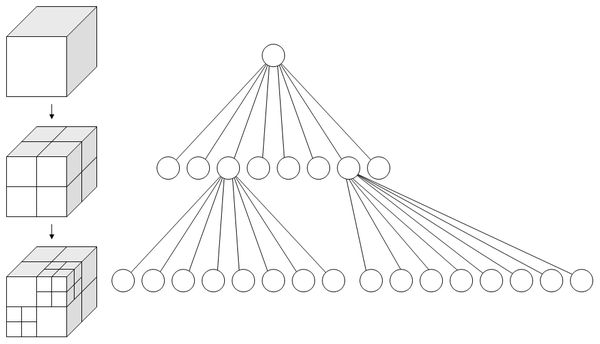
\includegraphics[width=0.8\linewidth]{octree.png}}
	\caption{Восьмеричное разбиение пространства}
	\label{fig:octree}
\end{figure}

Когда восьмеричное дерево построено, можно за время порядка $O(\log_8 N)$ находить вершину, ближайшую к любой заданной точке, а также эффективно рассчитывать электрическое поле. Для приблизительного расчёта поля от вершин, расположенных в достаточно далёком кубе, можно вычислить поле центра масс данного куба. При этом зависимость приемлемого размера такого <<куба~усреднения>> от расстояния до точки, в которой вычисляется поле, может быть задана произвольно. Таким образом алгоритм позволяет произвольно регулировать соотношение между скоростью и точностью вычислений. Время расчёта электрического поля во всех вершинах графа становится существенно меньше, чем $O(N^2)$.

\subsection{Программный код}
Программный пакет написан на языке C++ в соответствии с принципами объектно-ориентированного программирования. На текущий момент пакет состоит из, приблизительно, 15 тыс. строк кода. В разработке применяются следующие технологии и библиотеки:
\begin{itemize}
	\item \textbf{Параллелизация вычислений} выполняется при помощи библиотеки Intel TBB.
	\item \textbf{Вывод} состояния графа в файлы в формате VTK осуществляется при помощи библиотеки libVTK
	\item \textbf{Визуализация данных} в реальном времени реализована при помощи Qt и libVTK
	\item \textbf{Модульное тестирование} различных компонентов системы работает на основе библиотеки GTest
	\item \textbf{Прочие вспомогательные задачи} "--- разбор конфигурационных файлов, работа с командной строкой и т.п. осуществляются при помощи компонентов библиотеки Boost
	\item \textbf{Визуализация готовых расчётов,} генерация видео и оформление изображений для публикаций производится внешней программой ParaView.
\end{itemize}

Для большинства расчётов использовался сервер с двумя процессорами Intel Xeon E5-2660 @ 2.60GHz с общим количествов физических ядер 20\,шт., 128\,Гб ОЗУ (однако задаче требуется всего лишь 1-2\,Гб).

\section{Выводы}
Разработана транспортная самоорганизующаяся модель процесса инициации молнии, описывающая процессы от образования областей спонтанной проводимости до распространения и ветвления билидера. Разработан специализированный программный пакет для проведения расчётов модели. Продолжительность моделируемых процессов составляет порядка 1\,мс, пространственный масштаб проводящих структур "--- около 100\,м.

Модель обладает рядом уникальных особенностей: отсутствие пространственной сетки, неограниченная степень ветвления, учёт асимметрии возникновения положительных и отрицательных стримеров, самосогласованное моделирование стримерно-лидерного перехода при помощи параметризации ионизационно-перегревной неустойчивости.

Модель воспроизводит реалистичные макроскопические параметры разряда, такие, как ток в канале билидера, погонный заряд чехла лидера, скорость распространения лидера, поле в его канале. Воспроизводимая картина развития разряда соответствует экспериментальным наблюдениям. Таким образом, при помощи модели показано, что одного лишь механизма индукционного разделения заряда достаточно для возникновения билидера в докритическом поле облака при условии возникновения областей проводимости порядка~10-30\,см.

\FloatBarrier
           % Глава 2
%\include{Dissertation/part3}           % Глава 3
\chapter*{Заключение}                       % Заголовок
\addcontentsline{toc}{chapter}{Заключение}  % Добавляем его в оглавление

%% Согласно ГОСТ Р 7.0.11-2011:
%% 5.3.3 В заключении диссертации излагают итоги выполненного исследования, рекомендации, перспективы дальнейшей разработки темы.
%% 9.2.3 В заключении автореферата диссертации излагают итоги данного исследования, рекомендации и перспективы дальнейшей разработки темы.
%% Поэтому имеет смысл сделать эту часть общей и загрузить из одного файла в автореферат и в диссертацию:

В качестве основных результатов диссертации можно перечислить следующее:
%% Согласно ГОСТ Р 7.0.11-2011:
%% 5.3.3 В заключении диссертации излагают итоги выполненного исследования, рекомендации, перспективы дальнейшей разработки темы.
%% 9.2.3 В заключении автореферата диссертации излагают итоги данного исследования, рекомендации и перспективы дальнейшей разработки темы.
\begin{enumerate}
	\item Разработанная и введена в эксплуатацию региональная грозопеленгационная система OpenLDS. Проведено исследование точности системы и оценена погрешность позиционирования молниевых разрядов.
	
	\item На основе данных ГПС показано, что тип местности существенно влияет на грозовую активность в регионе. Выдвинута гипотеза об отрицательном влиянии мощных ТЭЦ на количество гроз. Показано, что максимумы и минимумы грозовой активности могут иметь локальный характер с характерным масштабом в 20\,км.	
	
	\item Проведён статистический анализ молниевой активности по данным ГПС на территории Нижегородской области. Количество гроз существенно зависит от типа местности и изменяется более, чем в 2,7 раз на территориях, удалённых на 20\,км, что сравнимо с размером грозового фронта. На основе полученных данных выдвинута гипотеза о влиянии мощных ТЭЦ на снижение количества гроз.
	
	\item На основе данных ГПС показано, что условная вероятность возникновения каждого последующего повторного обратного удара увеличивается до компоненты~№8, далее остаётся приблизительно неизменной. Данное поведение что свидетельствует о том, что средняя многокомпонентная молния не способна нейтрализовать большую часть доступного заряда и что прерывание цепочки повторных разрядов обеспечивается деградацией канала, а не нехваткой заряда в облаке.
	
	\item На основе данных ГПС показано, что средний интервал между повторными ударами монотонно увеличивается от 76\,мс до 110\,мс, что свидетельствует об усложнении процесса сбора заряда для каждой последующей компоненты.	
	
	\item Создана транспортная самоорганизующаяся модель стримерно-лидерной стадии процесса инициации молнии, обладающая рядом уникальных особенностей по сравнению с уже имеющимися моделями и основанная на оригинальном подходе. Модель корректно описывает качественные и количественные макроскопические процессы, не заложенные явно в её исходные принципы.
	
	\item На основе моделирования показано, что развитие молниевого разряда на стримерно-лидерной стадии возможно за счёт коллективных эффектов под действием электростатической индукции и не требует привлечения иных механизмов.	
\end{enumerate}
%И какая-нибудь заключающая фраза.

Автор благодарен своим коллегам и руководителям "--- члену-корреспонденту РАН, доктору физико-математических наук Марееву~Е.\,А., доктору физико-математических и биологических наук Иудину~Д.\,И., кандидату физико-математических наук и научному руководителю автора Шлюгаеву~Ю.\,В., научным сотрудникам ИПФ~РАН Ильину Н.\,С., Кутерину~Ф.\,А., Сысоеву~А.\,А. за совместную работу над задачами, вошедшими в данную диссертацию. Также, автор благодарен научным сотрудникам ИПФ~РАН Мартынову~В.\,О. и Оладышкину~И.\,В. за конструктивные замечания и моральную поддержку.      % Заключение
\include{Dissertation/acronyms}        % Список сокращений и условных обозначений
%\include{Dissertation/dictionary}      % Словарь терминов
\include{Dissertation/references}      % Список литературы
\include{Dissertation/lists}           % Списки таблиц и изображений (иллюстративный материал)

\setcounter{totalchapter}{\value{chapter}} % Подсчёт количества глав

%%% Настройки для приложений
\appendix
% Оформление заголовков приложений ближе к ГОСТ:
\setlength{\midchapskip}{20pt}
\renewcommand*{\afterchapternum}{\par\nobreak\vskip \midchapskip}
\renewcommand\thechapter{\Asbuk{chapter}} % Чтобы приложения русскими буквами нумеровались

%\include{Dissertation/appendix}        % Приложения

\setcounter{totalappendix}{\value{chapter}} % Подсчёт количества приложений

\end{document}
